% Uses `UCL Thesis LaTeX Template:  (c) Ian Kirker, 2014'
% 
% Note that the \input command just streams in whatever file you give
%  it, while the \include command adds a page break, and does some
%  extra organisation to make compilation faster. Note that you can't
%  use \include inside an \include-d file.
% We suggest using \input for settings and configuration files that
%  you always want to use, and \include for each section of content.
% If you do that, it also means you can use the \includeonly statement
%  to only compile up the section you're currently interested in.
% You might also want to put figures into their own files to be \input.

% For more information on \input and \include, see:
%  http://tex.stackexchange.com/questions/246/when-should-i-use-input-vs-include

% Formatting rules:
% https://www.ucl.ac.uk/students/exams-and-assessments/research-assessments/format-bind-and-submit-your-thesis-general-guidance

% This package goes first and foremost, because it checks all 
%  your syntax for mistakes and some old-fashioned LaTeX commands.
% Note that normally you should load your documentclass before 
%  packages, because some packages change behaviour based on
%  your document settings.
% Also, for those confused by the RequirePackage here vs usepackage
%  elsewhere, usepackage cannot be used before the documentclass
%  command, while RequirePackage can. That's the only functional
%  difference as far as I'm aware.
\RequirePackage[l2tabu, orthodox]{nag}


% ------ Main document class specification ------
% The draft option here prevents images being inserted,
%  and adds chunky black bars to boxes that are exceeding 
%  the page width (to show that they are).
% The oneside option can optionally be replaced by twoside if
%  you intend to print double-sided. Note that this is
%  *specifically permitted* by the UCL thesis formatting
%  guidelines.
%

%\documentclass[12pt,phd,draft,a4paper,oneside]{ucl_thesis}
\documentclass[12pt,phd,a4paper,oneside]{ucl_thesis}

\input{MainPackages}

%%
%% This file uses the hyperref package to make your thesis have metadata embedded in the PDF, 
%%  and also adds links to be able to click on references and contents page entries to go to 
%%  the pages.
%%

\RequirePackage[hyphens]{url}
\usepackage[bookmarks,pagebackref,hidelinks]{hyperref}

%This (in combo with pagebackred in hyperref) adds 'cited: p. X' after each bibliography entry
\renewcommand*\backref[1]{\ifx#1\relax \else (cited: p. #1) \fi}

\AtBeginDocument{
    \hypersetup{
        anchorcolor=purple,
        citecolor=green,
        pdfsubject={A thesis upon the subject of Museum Lighting, Colour Constancy and Melanopsin.},
        pdfkeywords={Museum Lighting, Colour Constancy, Chromatic Adaptation, Melanopsin},
        pdfauthor={Daniel Garside},
        pdftitle={Museum Lighting, Colour Constancy and Melanopsin},
    }
}

% Gives you the ability to add comments to pdfs
% This must be loaded after hyperref
%\usepackage[author={Danny Garside}]{pdfcomment}

%
% Creates hyperlinks automatically from DOIs, and allows for use of \doi{} rather than \url{} which means it can handle non-allowed characters in DOIs.
\usepackage{doi}

% uses standard font for URLs
\urlstyle{same}

\usepackage[acronym]{glossaries}
\loadglsentries[\acronymtype]{acro}


% And then some settings in separate files.
\input{FloatSettings} % For things like figures and tables
\bibliographystyle{plainnat}

\def\bibfont{\footnotesize}   % For bibliographies

\setcounter{secnumdepth}{3} %default 3

\makeglossaries

\begin{document}

% I may change the way this is done in a future version, 
%  but given that some people needed it, if you need a different degree title 
%  (e.g. Master of Science, Master in Science, Master of Arts, etc)
%  uncomment the following 3 lines and set as appropriate (this *has* to be before \maketitle)
% \makeatletter
% \renewcommand {\@degree@string} {Master of Things}
% \makeatother

\title{Museum Lighting, Colour Constancy and Melanopsin}
\author{Daniel Garside}
\department{Civil, Environmental and Geomatic Engineering}

\maketitle
\makedeclaration

\begin{abstract} % 300 word limit

% Extended abstract: 

%Light causes damage to objects in museums. Museums seek a pragmatic compromise between lighting which causes minimal damage to objects, and lighting which allows maximal visitor enjoyment. Generally this is achieved by following industry recommendations for maximum illuminance and colour rendering index.
%
%A complementary way to reduce damage, highlighted by the Commission Internationale de l'Eclairage in a 2004 publication, is to choose illumination of a lower Correlated Colour Temperature (CCT), because such illumination will contain most radiation energy in the longer wavelengths, which are generally less damaging to objects. Computations performed for a range of commercially available lighting products showed a strong correlation between predicted damage and CCT, with a factor of two between the low and high CCT sources. Practically, a sensitive object might be displayed for twice as long under a low CCT illuminant than a high one, before passing a damage threshold. 
%
%A series of interviews with museum professionals showed that this technique is not currently being employed. One reason is a belief that changing the CCT in an environment will affect the visual experience and the atmosphere in the room.
%
%Models of vision suggest that a change in CCT alone should not affect visual experience; that in a space with a single type of lighting we should be able to adapt to any colour of illumination. This seems at most only partially true. It is true that we adapt reasonably well to the ambient illumination, both in terms of luminance and chromaticity, such that our perception of object colours relates primarily to object reflectance properties rather than the absolute intensities reaching our eyes. Generally, however, we do also seem to have an awareness of the properties of the illumination in a scene, and even a preference for some sources over others. Historically, experiments seeking to find an ideal preferred CCT have provided conflicting results.
%
%One possible reason for these conflicting results might be that an additional retinal mechanism is involved in chromatic adaptation. The studies in this thesis have investigated whether a cell group called the `intrinsically photosensitive Retinal Ganglion Cells' (ipRGCs) might be involved in colour constancy. This cell group has traditionally been considered as having no output to visual pathways, and so colour constancy experiments haven't controlled for ipRGC activation, but recent research has shown that ipRGCs do in fact have a limited input to visual pathways. There are a range of reasons that suggest that they may play a role in colour constancy specifically.
%
%To investigate the effect of different levels of ipRGC activation on an observer's state of colour constancy,	two lab-based psychophysical experiments were performed. The first sought to examine the effect of different wavelengths of light upon chromatic adaptation. Within a Ganzfeld viewing environment, illuminated by one of 16 different wavelengths of near-monochromatic light, observers performed an achromatic setting task, controlling the chromaticity of a display visible in the central field through a 4° circular aperture with two handheld sliders.
%
%In the second experiment the role of melanopsin in chromatic adaptation was more directly questioned. The same task was performed as in the first experiment, but the Ganzfeld was this time illuminated by one of two perceptually metameric lights with different melanopic irradiance levels. Neither of these experiments provided evidence for a simple or strong effect of ipRGC activation, though this is limited to the case where peripheral stimulation would affect central perception.
%
%Concurrently, a method has been developed for performing colour constancy experiments outside of the lab environment, which can be completed quickly by naive observers in `real-life' illumination conditions. The method uses a tablet computer, on which an isoluminant plane through CIELUV is presented, successively varying in orientation and spatial offset. The observer is tasked with selecting, by touching with a finger, an achromatic point from within each stimulus. From the recorded selections an estimate of the observer's state of chromatic adaptation is computed.
%
%Following these experiments a different approach was adopted: rather than asking what was the affect of varying ipRGC activation upon experimental subjects, instead the question was posed whether an ipRGC-based signal could hypothetically be useful for colour constancy, considering what we know of daylight variability and natural surface reflectance properties. A computational methodology was employed. It was found that the spectral sensitivity of melanopsin is optimal for providing a signal that can transform raw chromatic signals to an illuminant-independent space, and that this can be done without using any scene level assumptions such as grey-world.
%
%The applied goal of this research was to increase our understanding of colour constancy so as to advise museums on how to reduce damage to objects without degrading visitor experience. Asking whether ipRGCs play a role in colour constancy is additionally valuable to the vision science community, and to lighting engineering applications beyond the museum world.
\end{abstract}

\begin{impactstatement}

%	UCL theses now have to include an impact statement. \textit{(I think for REF reasons?)} The following text is the description from the guide linked from the formatting and submission website of what that involves. (Link to the guide: {\scriptsize \url{http://www.grad.ucl.ac.uk/essinfo/docs/Impact-Statement-Guidance-Notes-for-Research-Students-and-Supervisors.pdf}})
%
%\begin{quote}
%The statement should describe, in no more than 500 words, how the expertise, knowledge, analysis,
%discovery or insight presented in your thesis could be put to a beneficial use. Consider benefits both
%inside and outside academia and the ways in which these benefits could be brought about.
%
%The benefits inside academia could be to the discipline and future scholarship, research methods or
%methodology, the curriculum; they might be within your research area and potentially within other
%research areas.
%
%The benefits outside academia could occur to commercial activity, social enterprise, professional
%practice, clinical use, public health, public policy design, public service delivery, laws, public
%discourse, culture, the quality of the environment or quality of life.
%
%The impact could occur locally, regionally, nationally or internationally, to individuals, communities or
%organisations and could be immediate or occur incrementally, in the context of a broader field of
%research, over many years, decades or longer.
%
%Impact could be brought about through disseminating outputs (either in scholarly journals or
%elsewhere such as specialist or mainstream media), education, public engagement, translational
%research, commercial and social enterprise activity, engaging with public policy makers and public
%service delivery practitioners, influencing ministers, collaborating with academics and non-academics
%etc.
%
%Further information including a searchable list of hundreds of examples of UCL impact outside of
%academia please see \url{https://www.ucl.ac.uk/impact/}. For thousands more examples, please see
%\url{http://results.ref.ac.uk/Results/SelectUoa}.
%\end{quote}
\end{impactstatement}

\begin{acknowledgements}
% Acknowledge all the things!

% I also wish to note my appreciation and thanks to the various pieces of open source software I used in the writing of this thesis. For further details see Appendix \ref{appendixlabel3}.

% Re:tablet - Thanks are given to: the museum staff at the Grant Museum and British Museum, the staff at UCL PAMELA, and the experimental participants.

% Keats

% PTB

\end{acknowledgements}

\setcounter{tocdepth}{2} 
% Setting this higher means you get contents entries for
%  more minor section headers.

\tableofcontents
\listoffigures
\printglossary[type=\acronymtype,style=long]
\glsresetall %resets glossary counter so that the long use in the list of figures doesn't count as the first use 
%\listoftables


%\chapter{Introduction}
\label{chapterlabel1}

\section{Context}
Light causes damage to objects in museums. Museums seek a pragmatic compromise between lighting which causes minimal damage to objects, and lighting which allows maximal visitor enjoyment. Generally this is achieved by following industry recommendations for maximum illuminance and \gls{CRI}.

A complementary way to reduce damage, highlighted by the \gls{CIE} in a 2004 publication \citep{cie_cie_2004}, is to choose illumination of a lower \gls{CCT}, because such illumination will contain most radiation energy in the longer wavelengths, which are generally less damaging to objects. To verify and extend the work of the \gls{CIE}, a \gls{DI} was calculated for a range of commercially available lighting products (\textbf{Section \ref{sec:CCTmus}}). This showed a strong correlation between predicted damage and \gls{CCT}, with a factor of two between the low and high \gls{CCT} sources. Practically, a sensitive object might be displayed for twice as long under a low \gls{CCT} light source than under a high \gls{CCT} light source, before passing a particular damage threshold. 

A series of interviews with museum professionals showed that this technique is not currently being employed (\textbf{Chapter \ref{chap:Interviews}}). One reason is a belief that changing the \gls{CCT} in an environment will affect the visual experience and the atmosphere in the room.

Most models of vision suggest that a change in \gls{CCT} alone, within moderate limits, should not affect visual experience; that in a space with a single type of lighting we should be able to adapt to any colour of illumination. This seems at most only partially true. It is true that we adapt reasonably well to the ambient illumination, both in terms of luminance and chromaticity, such that our perception of object colours relates primarily to object reflectance properties rather than the absolute intensities reaching our eyes. Generally, however, we do also seem to have an awareness of the properties of the illumination in a scene, and even a preference for some sources over others. Historically, experiments seeking to find an ideal preferred \gls{CCT} have provided conflicting results.

One possible reason for these conflicting results might be if an additional retinal mechanism is involved in chromatic adaptation. The studies in this thesis have investigated whether a cell group called the \glspl{ipRGC} might be involved in colour constancy. This cell group has traditionally been considered as having no output to visual pathways, and so colour constancy experiments haven't controlled for \gls{ipRGC} activation, but recent research has shown that \glspl{ipRGC} do in fact have a limited input to visual pathways (see Section \ref{sec:ipRGCbeyond}). There are a range of reasons which suggest that they may play a role in colour constancy specifically.

\section{Research Question}

The principal research question considered in this thesis is: \textbf{Are \glspl{ipRGC} involved in colour constancy?}

If they are, this may explain why previous investigations into preferred \gls{CCT} have produced conflicting results. If we can understand how they are involved, this may give us a new insight into how to vary the \gls{CCT} of museum illumination in such a way that we can limit damage without degrading visitor experience.

\section{Chapter Summaries}

To better understand how museum professionals currently make lighting decisions (what metrics they use, what the guidance is for using these metrics, what the current challenges and limitations are) a series of interviews was performed with museum lighting professionals \citep{garside_how_2017}. The responses to these interviews are summarised in \textbf{Chapter \ref{chap:Interviews}}.

To investigate the effect of different levels of \gls{ipRGC} activation on an observer's state of colour constancy, two lab-based psychophysical experiments were performed (\textbf{Chapters \ref{chap:LargeSphere} and \ref{chap:SmallSphere}}). The first sought to examine the effect of different wavelengths of light upon chromatic adaptation. Within a Ganzfeld viewing environment, illuminated by one of 16 different wavelengths of near-monochromatic light, observers performed an achromatic setting task, controlling the chromaticity of a display visible in the central field through a 4$^{\circ}$ circular aperture with two handheld sliders.

In the second experiment the role of melanopsin in chromatic adaptation was more directly questioned. The same task was performed as in the first experiment, but the Ganzfeld was this time illuminated by one of two perceptually metameric lights with different melanopic illuminance levels. Neither of these experiments provided evidence for a simple or strong effect of ipRGC activation.

Concurrently, a method has been developed for performing colour constancy experiments outside of the lab environment, which can be completed quickly by naive observers in `real-world' conditions (\textbf{Chapter \ref{chap:Tablet}}). The method uses a tablet computer, upon which an isoluminant plane through CIELUV is presented, successively varying in orientation and spatial offset. The observer is tasked with selecting, by touching with a finger, an achromatic point from within each stimulus. From the recorded selections an estimate of the observer's state of chromatic adaptation is computed.

Following these experiments a different approach was adopted: rather than asking what was the effect of varying \gls{ipRGC} activation upon experimental subjects, instead the question was posed whether an \gls{ipRGC}-based signal could hypothetically be useful for colour constancy, considering what we know of daylight variability and natural surface reflectance properties (\textbf{Chapter \ref{chap:Melcomp}}). A computational methodology was employed for this exploratory study. It was found that a simple transform can be made from raw signals to an illuminant independent space, with the use of a melanopsin-based signal. Further, it was found that the spectral sensitivity of melanopsin is near-optimal for providing a signal for such a transformation, and that this can be done without using any scene level assumptions such as `grey-world'.

\textbf{Chapter \ref{chap:Conclusions}} provides a summary and discussion of results, and suggests routes for future work.

\section{Associated Publications}

{\parindent0pt \footnotesize


\subsection*{Journal Papers}

\textbf{Daniel Garside}, Katherine Curran, Capucine Korenberg, Lindsay MacDonald, Kees Teunissen, and Stuart Robson. How is museum lighting selected? An insight into current practice in UK museums. \textit{Journal of the Institute of Conservation}, 40(1):3-14, January 2017. \doi{10.1080/19455224.2016.1267025}

\subsection*{Conference Papers}

\textbf{Daniel Garside}. Initial Observations on Lighting Situations in The British Museum. In \textit{1st International Conference, Science and Engineering in Arts, Heritage and Archaeology}, page 58, London, UK, July 2015. \doi{10.6084/m9.figshare.4269665.v1}
\bigskip

\textbf{Daniel Garside}, Katherine Curran, Capucine Korenberg, Lindsay MacDonald, Kees Teunissen, and Stuart Robson. Interviewing Museum Professionals: How is Museum Lighting Selected? In \textit{SEAHA (Science and Engineering in Arts, Heritage and Archaeology)}, Oxford, UK, June 2016. \doi{10.6084/m9.figshare.5840952.v1}
\bigskip

\textbf{Daniel Garside}, Lindsay MacDonald, Kees Teunissen, Katherine Curran, Capucine Korenberg, and Stuart Robson. Potential uses for spectrally variable lighting in museum environments. In \textit{Progress in Colour Studies (PICS)}, page 100, London, UK, September 2016. \doi{10.6084/m9.figshare.4269659.v1}
\smallskip %This one appears to create a bigger gap for some reason

\textbf{Daniel Garside}, Lindsay MacDonald, Kees Teunissen, and Stuart Robson. Estimating Chromatic Adaptation in a Museum Environment Using a Tablet Computer. In
\textit{Proceedings of AIC 2016 Interim Meeting - Color in Urban Life: Images, Objects and Spaces}, pages 125-129, Santiago, Chile, October 2016. \doi{10.6084/m9.figshare.4269680.v2}
\bigskip

Lindsay MacDonald and \textbf{Daniel Garside}. Adapting to a Chromatic Environment. In \textit{Proceedings of AIC 2016 Interim Meeting - Color in Urban Life: Images, Objects and Spaces}, pages 109-113, Santiago, Chile, October 2016.
\bigskip

\textbf{Daniel Garside} and Lindsay MacDonald. Investigations into the effect of different spectra upon the process of chromatic adaption. In \textit{Proceedings of the International Colour Vision Symposium (ICVS)}, page 35, Erlangen, Germany, August 2017.
\bigskip

\textbf{Daniel Garside}. Light art as a pedagogical tool for teaching the science of colour perception. In \textit{Abstracts from the 5th Visual Science of Art Conference (VSAC)}, page 381, Berlin, Germany, August 2017. \doi{10.1163/22134913-00002099}
\bigskip

\textbf{Daniel Garside}, Stuart Robson, Lindsay MacDonald, Katherine Curran, Kees Teunissen, and Capucine Korenberg.  A method for performing colour constancy studies using a tablet computer. In \textit{European Conference on Visual Perception (ECVP)}, Berlin, Germany, August 2017. \doi{10.6084/m9.figshare.5478493.v1}
\bigskip

M. Hess, \textbf{D. Garside}, T. Nelson, S. Robson, and T. Weyrich.  Object-Based Teaching and Learning for a Critical Assessment of Digital Technologies in Arts and Cultural Heritage. In \textit{ISPRS - International Archives of the Photogrammetry, Remote Sensing and Spatial Information Sciences, volume XLII-2-W5}, pages 349-354, Ottawa, Canada, August 2017. Copernicus GmbH. \doi{10.5194/isprs-archives-XLII-2-W5-349-2017}
\bigskip

L. W. MacDonald, \textbf{D. Garside}, and C. Teunissen. Melanopsin and Colour Vision. In \textit{Proceedings of 13th AIC Congress}, Jeju, South Korea, Oct 2017.
\bigskip

E. K. Webb, S. Robson, L. MacDonald, \textbf{D. Garside}, and R. Evans. Spectral and 3d Cultural Heritage Documentation Using a Modified Camera. In \textit{ISPRS - International Archives of the Photogrammetry, Remote Sensing and Spatial Information Sciences, volume XLII-2}, pages 1183-1190, Riva del Garda, Italy, May 2018. \doi{10.5194/isprs-archives-XLII-2-1183-2018}
\bigskip

\textbf{Daniel Garside}. Is there a role for melanopsin in chromatic adaptation? At \textit{The 16th International Symposium on the Science and Technology of Lighting (LS16)}, Sheffield, UK, June 2018.
\bigskip


\textbf{Daniel Garside}, Lindsay MacDonald, and Kees Teunissen. Does the spectral sensitivity of melanopsin in ipRGCs suggest a role in chromatic adaptation?  In \textit{Vision Sciences Society Annual Meeting Abstract, volume 18}, page 877, St Pete Beach, Florida, September 2018 \doi{10.1167/18.10.877}
\bigskip

\textbf{Daniel Garside} and Lindsay MacDonald. Assessing the effectiveness of a melanopsin-based signal for colour constancy. In \textit{Proceedings of the International Colour Vision Symposium (ICVS)}, page 65, Riga, Latvia, July 2019. 
\bigskip

\subsection*{Editorial Contributions}
A. Pokorska, P. Andrikopoulos, \textbf{D. Garside}, and C. Coon, editors. Book of Abstracts, Museum Lighting Symposium and Workshops.  \textit{1st International Museum Lighting Symposium \& Workshops}, London, UK, September 2017. \doi{10.14324/000.bk.10048078}

}

\section{Affiliations}
This project was supported by an EPSRC (Engineering and Physical Sciences Research Council) iCASE (Industrial Cooperative Awards in Science \& Technology) studentship, with industry sponsors Signify Research (née Philips Lighting Research) and The British Museum.

Signify Research provided financial and technical support, with supervision from Kees Teunissen. The British Museum provided technical support and access to facilities, with supervision from Capucine Korenberg. 

The project was supervised by Stuart Robson, Katherine Curran, Lindsay MacDonald, Kees Teunissen and Capucine Korenberg.

The thesis was examined by Anya Hurlbert (Newcastle University) and John Greenwood (University College London).
\chapter{Literature Review}
\label{LitReview}

This chapter shall provide summaries of the background information required to understand the content of this thesis, and also review the state of the art of the various subjects that this thesis covers.

\section{Colour Science}

Organisms on earth posses visual systems such that they can glean information about spatially remote objects through the sensing of light reflected from these objects towards the organism. They are able to do this because the sun emits electromagnetic radiation (which we call `light' when it is within our visual sensitivity range), our atmosphere transmits many parts of this radiation (absorbing some wavelengths more so than others), and objects absorb some and reflect some of this radiation (again, some wavelengths more so than others), as shown in Figure \ref{fig:SPD}.
%minnaert?

\begin{figure}[hbtp]
\includegraphics[max width=\textwidth]{figs/LitRev/daylightAndBananas.pdf}
\caption{The \gls{SPD} of a single measurement of daylight (sunlight plus scattered blue-sky light, from \citet{hernandez-andres_color_2001}) and the light reflected from 2 different surfaces - a green banana and a yellow banana (data from personal correspondence with David Slaughter after \citet{li_optical_1997}), computed by multiplying the \gls{SPD} by the measured \glspl{SRF} of the two surfaces. \Glspl{SPD} normalised such that the max of the daylight \gls{SPD} is 1.}
\label{fig:SPD}
\end{figure}

Our perception of colour generally correlates with the way in which objects preferentially reflect some wavelengths over others (described by the \acrfull{SRF}) which assists in the recognition of objects (that's a banana) and the discrimination of distinct objects, often in a manner that is ecologically beneficial (that's a \emph{ripe} banana).

\newpage

\subsection{Colorimetry}

\textit{The current recommended source for colorimetry is \gls{CIE} document `\gls{CIE} 015:2018'\citep{cie_cie_2018}\footnote{Though as \citet{fairchild_cie_2019} notes, this document is `expensive and somewhat difficult to find', and as such I have been using a draft of the now superseded `\gls{CIE} 15.3:2004'\citep{cie_cie_2004-2} as my personal guide.}. Whlist this is the authoritative reference, my personal opinion is that an understanding of colorimetry of \gls{CIE} colorimetry is best gained from an understanding of it's history, and for this I recommend Janos Schanda's book `Colorimetry: Understanding the \gls{CIE} System'\citep{schanda_colorimetry_2007}.}

\bigskip

Colorimetry is the study of the quantitative specification of colour. As a subjective, internal and anthropocentric concept, in order to measure anything meaningful and comparable, we use a standard observer, or more precisely, one of a number of defined standard observers \cite{cie_bs_2011}.

The classic standard observer was defined by the \gls{CIE} in 1931, following experiments by Wright and Guild \cite{wright_re-determination_1929, guild_colorimetric_1931}. Despite several more recently published standard observers, the 1931 observer is still much used, and I shall use it in the following example of how a basic colorimetric computation is performed.

\glsreset{SPD}
\glsreset{SRF}
\glsreset{CMF}
\glsreset{SSF}

An illuminant is defined by its \gls{SPD}, a surface as it's \gls{SRF}, and a the sensitivity of a sensor (such as a photosensitive cell in the retina, or a pixel in a camera) by its \gls{CMF} (or in the case that biologically based measurements are used - the \gls{SSF}).

\begin{figure}[htbp]
\includegraphics[max width=\textwidth]{figs/LitRev/SPDetc.pdf}
\caption{An \gls{SPD} (D65), a set of \glspl{SRF} (from a Macbeth Colour Checker) and three \glspl{CMF} (\gls{CIE} 1931 observer).}
\label{fig:specFun}
\end{figure}
% % How is D65 normalised here?

The light reaching the eye for a given reflecting surface under a given illuminant (termed the `colour signal') can be computed by multiplying the \gls{SPD} by the \gls{SRF} at each sampled interval.

\begin{equation}
\phi(\lambda)=R(\lambda) \cdot S(\lambda)
\end{equation}

where $R(\lambda)$ is the \gls{SRF}, $R(\lambda)$ is the \gls{SPD} and $\phi(\lambda)$ is the resulting colour signal. From this a set of values termed `tristimulus values' may be computed. Tristimulus values are computed by multiplying the colour signal by the \glspl{CMF} or \glspl{SSF}, and following the principle of univariance (that each cone type cannot alone distinguish between different wavelengths) the tristimulus values can, to some extent, be thought of as containing the entirety of the chromatic information about a surface (excluding high level colour appearance phenomena predicted by \Glspl{CAM}, and properties such as gloss).

\begin{subequations}
\begin{align}
X=k \sum_{\lambda} \phi(\lambda) \overline{x}(\lambda) \Delta \lambda \\ 
Y=k \sum_{\lambda} \phi(\lambda) \overline{y}(\lambda) \Delta \lambda \\ 
Z=k \sum_{\lambda} \phi(\lambda) \overline{z}(\lambda) \Delta \lambda
\end{align}
\label{eq:XYZ}
\end{subequations}

\nopagebreak %this doesn't work currently

where $\overline{x}(\lambda)$ (said `x bar'), $\overline{y}(\lambda)$ and $\overline{z}(\lambda)$ are the \glspl{CMF} of the 1931 observer (or are replaced by the \Glspl{CMF}/\Glspl{SSF} or the chosen observer), $\phi(\lambda)$ is as defined above, $k$ is a normalising factor, and it is recommended that $\Delta\lambda$ be 1nm. It is traditional to set $k$ such that $Y=100$, though in the case of relative colorimetry (most cases) is often ignored since the following equation renders it superfluous.

From the tristimulus values chromaticity co-ordinates ($x$ and $y$) can be computed. These can then be plotted on a 1931 chromaticity space diagram, shown as Figure \ref{fig:1931}.

\begin{subequations}
\begin{align}
x=\frac{X}{X+Y+Z} \\
y=\frac{Y}{X+Y+Z} 
\end{align}
\label{eq:1931chrom}
\end{subequations}

% Here's a \gls{MATLAB} example, using \gls{PTB} for data:

% \begin{lstlisting}[language=MATLAB]
% load spd_D65 % SPD: CIE D-series illuminant D65
% load sur_macbeth % SRF: macbeth colour checker
% load T_xyz1931 % CMF: CIE 1931

% colourSignals = sur_macbeth.*spd_D65;
% XYZ = T_xyz1931*colourSignals;
% xy = [XYZ(1,:)./sum(XYZ);XYZ(2,:)./sum(XYZ)];
% \end{lstlisting}

% Plotting: 

% \begin{lstlisting}[language=MATLAB]
% spectralLocus = [T_xyz1931(1,:)./sum(T_xyz1931);T_xyz1931(2,:)./sum(T_xyz1931)];
% sRGBSpectralLocus = XYZToSRGBPrimary(T_xyz1931);

% figure, hold on, 
% scatter(spectralLocus(1,1:70),spectralLocus(2,1:70),[],sRGBSpectralLocus(:,1:70)','filled')
% scatter(xy(1,:),xy(2,:),'k')
% axis equal, axis([0 1 0 1])
% xticks([0 1]), yticks([0 1])
% xlabel('x'), ylabel('y')
% \end{lstlisting}

\begin{figure}[htbp]
\includegraphics[max width=\textwidth]{figs/LitRev/ColorimetryDemo1.pdf}
\caption{The \gls{CIE} 1931 chromaticity space, showing the chromaticity of the macbeth colour checker patches under D65. Note that for all of the plots in this section, the colours used for the spectral loci are only very rough approximations.}
\label{fig:1931}
\end{figure}

\subsubsection{Specific Colour Spaces}

Over time various other colour spaces have been proposed and formally accepted by the \gls{CIE}, each aiming to improve upon a prior space in one or more ways. One of the most frequently sought characteristics for a colour space is perceptual uniformity, whereby a set distance in one part of the space is comparable in terms of apparent colour difference to that same distance in another part of the space.

One such chromaticity space which shall be used extensively in this thesis is the \gls{CIE} 1976 UCS (uniform chromaticity scale) space, which is a relatively simple transformation of the 1931 chromaticity space. The conversion can be accomplished in a number of analogous fashions, one of which is shown below.

\begin{subequations}
\begin{align}
u' &= 4x / (-2x + 12y + 3) \\
v' &= 9y / (-2x + 12y + 3)
\end{align}
\end{subequations}

where $x$ and $y$ are the 1931 chromaticity co-ordinates as defined in Equation \ref{eq:1931chrom}. The data presented in Figure \ref{fig:1931} are re-plotted in this new space in Figure \ref{fig:UCS}.

\begin{figure}[htbp]
\includegraphics[max width=\textwidth]{figs/LitRev/ColorimetryDemo3.pdf}
\caption{\gls{CIE} 1976 UCS (uniform chromaticity scale) space, showing the chromaticity of the macbeth colour checker patches under D65 (as in Figure \ref{fig:1931}).}
\label{fig:UCS}
\end{figure}

A three-dimensional extension to the CIE 1976 UCS space is the \gls{CIE} 1976 L*u*v* colour space, often abbreviated to CIELUV, which aims to provide perceptual uniformity in a space that includes both chromaticity and lightness (relative to a white object under the same illumination). It is defined as follows:

\begin{subequations}
\begin{align}
L^{*} &= 116 f(Y/Y_{n})-16 \\
\textrm{where} f(Y/Y_{n}) &= (Y/Y_{n})^{1/3} &\textrm{ if } (Y/Y_{n}) > (24/116)^{3} \\
\textrm{or} f(Y/Y_{n}) &= (841/108)(Y/Y_{n})+16/116 &\textrm{ if } (Y/Y_{n}) \leq (24/116)^{3} \\
u^{*} &= 13L^{*}(u'-u'_{n}) \\ 
v^{*} &= 13L^{*}(v'-v'_{n})
\end{align}
\end{subequations}

where $Y_{n}$, $u'_{n}$ and $v'_{n}$ refer to the colour stimulus of a perfect reflector. The same data presented in Figures \ref{fig:1931} and \ref{fig:UCS} is presented in CIELUV in Figure \ref{fig:CIELUV} (though of course the three-dimensional quality of the data is somewhat lost).

\begin{figure}[htbp]
\includegraphics[max width=\textwidth]{figs/LitRev/ColorimetryDemo4.pdf}
\caption{A representation of CIELUV, showing the values for the macbeth colour checker patches under D65 (as in Figure \ref{fig:1931} and \ref{fig:UCS}). Note that if viewed from above, the distribution of points would appear similar to as in Figure \ref{fig:UCS}. If all of the points were of uniform L*, then the distribution would be identical, only with different scaling.}
\label{fig:CIELUV}
\end{figure}

Introduced at the same time as CIELUV was a colourspace with a similar goal of perceptual uniformity: CIELAB. They are similar in many ways, and share $L^{*}$ and if the CIE committee in charge of recommending such a space for adoption had been able to decide upon one or the other, one would have sufficed. As it is, both exist. CIELAB seems to be in slightly more common usage, but CIELUV is used in this thesis (particularly Chapter \ref{chap:Tablet}) due to the close link to an associated chromaticity space (the CIE 1976 UCS space). CIELAB is defined as follows:

\begin{subequations}
\begin{align}
L^{*} &= 116 f(Y/Y_{n})-16 \\
\textrm{where} f(Y/Y_{n}) &= (Y/Y_{n})^{1/3} &\textrm{ if } (Y/Y_{n}) > (24/116)^{3} \\
\textrm{or} f(Y/Y_{n}) &= (841/108)(Y/Y_{n})+16/116 &\textrm{ if } (Y/Y_{n}) \leq (24/116)^{3} \\
a^{*} &= 500[f(X/X_{n}) - f(Y/Y_{n})] \\ 
b^{*} &= 200[f(Y/Y_{n}) - f(Z/Z_{n})] \\
\end{align}
\end{subequations}

where $f(X/X_{n})$ and $f(Z/Z_{n})$ follow the same format as $f(X/X_{n})$.

The final colour space presented here is the \acrfull{MB} colour space. This space does not aspire to be perceptually uniform\footnote{This can be clearly noted by comparing Figure \ref{fig:lrMB} with previous figures. Where this set of chromaticities previously spanned the spaces fairly broadly, here all the chromaticities inhabit only a small portion of the chromaticity space.}. Instead, it aspires to provide a colour space which has a physiological underpinning. As such, the observer used consists of nominal \glspl{SSF} (rather than \glspl{CMF}), and the conversion from tristimulus values to chromaticity space attempts to mirror the way in which this actually occurs physiologically.

It was originally proposed by \citet{macleod_chromaticity_1979}, but was recently revised and endorsed by the \gls{CIE}, in documents `CIE 170-1:2006'\citep{cie_cie_2006} and `CIE 170-2:2015'\citep{cie_cie_2015}\footnote{I understand that the final publication in the series (`CIE 170-3:XXXX') is in preparation.}. The revisions included the definition of a new observer, based on the work of \citet{stockman_spectral_1999} and \citet{stockman_spectral_2000}, and the introduction of a set of new normalising terms, such that it is now calculated as follows.

\begin{subequations}
\begin{align}
L_{\text{MB}}&=k_{l} \sum_{\lambda} \phi(\lambda) \overline{l}(\lambda) \Delta \lambda \\ 
M_{\text{MB}}&=k_{m} \sum_{\lambda} \phi(\lambda) \overline{m}(\lambda) \Delta \lambda \\ 
S_{\text{MB}}&=k_{s} \sum_{\lambda} \phi(\lambda) \overline{s}(\lambda) \Delta \lambda
\end{align}
\label{eq:MBTristim}
\end{subequations}

where $k_{l}$ = 0.68990272, $k_{m}$ = 0.34832189, $k_{s}$ = 0.03715971. This set differs minimally but purposefully from Equation \ref{eq:XYZ}; in the choice of observer ($\overline{lms}$), and in the use of different scaling factors for each tristimulus value. \gls{MB} chromaticity values are then calculated as follows:

\begin{subequations}
\begin{align}
l_{\text{MB}}&= \frac{L_{\text{MB}}}{L_{\text{MB}}+M_{\text{MB}}} \\ 
s_{\text{MB}}&= \frac{S_{\text{MB}}}{L_{\text{MB}}+M_{\text{MB}}} 
\end{align}
\label{eq:MB}
\end{subequations}

Whereas the relationship between the axes of previous colour spaces was important, here the axes are nominally independent (representing different post-receptoral mechanisms) and so the scaling between the axes is arbitrary. The same data as presented previously is presented again in Figure \ref{fig:lrMB} in a \gls{MB} chromaticity space.

\begin{figure}[htbp]
\includegraphics[max width=\textwidth]{figs/LitRev/ColorimetryDemo5.pdf}
\caption{A \gls{MB} chromaticity space diagram (as per \gls{CIE} 170-2:2015\citep{cie_cie_2015}) showing the values for the macbeth colour checker patches under D65, as in previous figures.}
\label{fig:lrMB}
\end{figure}

\clearpage
\subsection{Colour rendering}

Colour rendering indices provide an indication of the colour appearance of objects under a test illumination. Colour fidelity indices (properly a subset of colour rendering indices, however the most commonly used colour rendering index is in fact a colour fidelity index) are designed to describe how well a light source will produce a faithful appearance in terms of corresponding colorimetry to an appearance under \gls{CIE} D-series illuminant (daylight proxy) or a black body radiator. %Target values are generally provided in museum lighting guidelines \citep{ies_ies_1996,druzik_guidelines_2012,cibse_lighting_2015,thomson_museum_1986}. The recommended value for the ubiquitously used \gls{CIE}~R\textsubscript{a} (As defined in \gls{CIE} 13.3:1995 \citep{cie_cie_1995}), often informally referred to as `CRI', varies from publication to publication, but is generally \gls{CIE}~R\textsubscript{a}$>$80, but with no experimental work referenced to support this figure. 
Research in colour rendering is at a point of change and development, with the recognition that a single figure might never be enough to describe the complex, multidimensional, subjective and context dependent qualia of colour rendering \citep{rea_color_2008}. Thus new indices, and modifications and addenda to long-established indices are being proposed \citep{smet_memory_2012,davis_color_2010,rea_practical_2010,ies_ies_2015,teunissen_characterising_2016}.

If we were to take a bunch of balloons (or any objects, but balloons provide a simple and vivid image) of varied and multiple colours, from an area lit with daylight to an area lit with artificial light, and the colour appearance changes, for example the colours become more dull, we would generally be disappointed. In this case, we could say that we were dissatisfied by the colour rendering qualities of the artificial light source. If the colours remained the same we probably would think little of it, but if we were pressed for a comment, we might say that the colour appearance was satisfactory. 

If the balloons stayed the same colour as they had been under daylight, we would be witnessing a high level of colour fidelity (fidelity meaning faithfulness or truthfulness). If fidelity aligns well with the priorities of the user, then high levels of fidelity are desirable. If the appearance of the balloons had changed in some other way than becoming more dull - for example the colours became more vivid or the hue of certain balloons changed drastically, we might not neccessarily be disappointed, but this would still represent a situation where we were witnessing poor fidelity.

Generally when discussing colour fidelity, we are actually discussing fidelity to appearance under daylight or sometimes a Planckian radiator, aka a black body radiator. This is a fine comparison, but one which should be consciously considered; fidelity is not a measure of a light source per se, it is a comparison of that light source to a reference illuminant.

Fidelity has long been considered semi-analogous for colour rendering as a whole, but it is really only one element of colour rendering\footnote{Here I should point out that the \gls{CIE} definition of colour rendering, from the publication \gls{CIE} S 017/E:2011 ILV: International Lighting Vocabulary \citep{cie_cie_2011} reads: ``Effect of an illuminant on the colour appearance of objects by conscious or subconscious comparison with their colour appearance under a reference illuminant.'' You might notice the similarities to the definition I have ascribed to colour fidelity, and specifically not colour rendering. This is an unfortunate clash of nomenclature which I see as inappropriate usage on the part of \gls{CIE}, and at some point I hope this official definition will be updated to match the modern vernacular.}. When considering how `good' a light source is at facilitating colour with the objects which it illuminates, we might consider different measures alongside or in place of fidelity.

\begin{itemize}
\item \emph{Colour Fidelity (to recap)} - A measure of comparison between how colours appear under daylight (or other reference) and how they appear under another light source. %Do the balloons appear the same colour indoors and out? Are individual colours important or is an average suitably representative?
\item \emph{Chromatic Discrimination} - The ability of a light source to illuminate objects such that subtle differences in colour are made most visible. %Can you tell the difference between all the balloons? How big are the differences? Are threshold differences more or less important than the perceived magnitude of suprathreshold differences?
\item \emph{Observer Preference} - Subjective preferences for the colour of objects, potentially related to an increase in saturation, or an observer's memory of colours, or specific colour effects (e.g. increased saturation of skin tones). %Do the balloons look `nicer'/more vivid/more like the last time you saw them?
\end{itemize}

These areas overlap, and often exhibit correlation. For example, if a light source has properties which allow for high fidelity rendering, quite often that light source might also allow for good colour discrimination and also facilitate colours which might appear natural and/or pleasing. These are not reliable correlations however; it is quite possible to have a light source with very dissimilar properties to daylight that could score highly on discrimination and/or preference, or vice versa.

The index in widest use currently for quantifying colour rendering is \gls{CIE}~R\textsubscript{a} (The General Colour Rendering Index). At the beginning of this doctoral project, this metric was used almost exclusively to generate the figure listed as `CRI' on the packaging for bulbs available commercially. %In the intervening time, \gls{IES} RP-30-15 \citep{ies_ies_2015}, and more recently \gls{IES} RP-30-18 \citep{ies_ies_2018}, have been published and have found considerable uptake from manufacturers.

\gls{CIE}~R\textsubscript{a} is a colour fidelity metric, produced by computing the colour differences of 8 specified \glspl{TCS}, between the situation where illumination is provided by the test source and that where it is provided by a reference illuminant with the same \gls{CCT} as the test source, and taking the arithmetic mean of these colour differences. The index is scaled such that the highest score is 100, for light sources which reproduce the \gls{TCS} set under the reference illuminant exactly, with any light source which induces a colour shift receiving a value less than 100, descending below 0 if the magnitude of the shifts are great enough.

The most recent version of the standard specifying this metric is `\gls{CIE} 13.3-1995 Method of Measuring and Specifying Colour Rendering Properties of Light Sources' \citep{cie_cie_1995}. This document briefly overviews the history of, and necessity for, a colour rendering index and highlights areas of the procedure which vary compared to previous recommendations, and clearly details the recommended procedure. The process is summarised in the flow chart of Figure \ref{fig:criflow}. For a worked example see \citet[p.388]{hunt_measuring_2011}.

In response to a lack of confidence that \gls{CIE}~R\textsubscript{a} delivered meaningful values for \gls{LED} illumination, a considerable amount of research and discussion has revolved around the subject of a colour rendering index to supersede \gls{CIE}~R\textsubscript{a}. This is commonly complicated by the incorrect assumption that the values obtained from a fidelity index in some way correlate with preference. A more valid criticism of \gls{CIE}~R\textsubscript{a} is that it comprises deprecated methods (for example, use of the \gls{CIE} 1960 UCS color space, now superseded) and data sets (a rather limited set of \glspl{TCS}, drawn from measurements of Munsell papers) for computing intermediary stages within the process of calculation, and thus this theoretically limits the `correctness' of any values produced by it.

Following many years where multiple \gls{CIE} technical committees aimed to deliver updated colour rendering indices, but subsequently didn't make any firm recommendations, an \gls{IES} group was formed with the aim of examining the issue. The output of this \gls{IES} group was the production of \gls{IES} TM-30-15\cite{ies_ies_2015}, which follows the same philosophy as \gls{CIE}~R\textsubscript{a} but with more modern colour science. It is still a contentious issue whether this updated index genuinely offers advantages over \gls{CIE}~R\textsubscript{a}. 
% it also includes a bunch of other things...
% and IES TM-30-18?

Alternative propositions which offer fundamentally different approaches to the evaluation of colour rendering have been offered in recent years, including: 
\begin{itemize}
\item indices based on production of memory colours \citep{smet_memory_2012}.
\item indices which consider the size of the gamut of a \gls{TCS} set \citep{rea_color_2008,teunissen_characterising_2016}.
\item indices which are fundamentally fidelity indices but which penalise or reward specific traits known to be disliked/preferred \citep{ohno_rationale_2010}.
\end{itemize}

\begin{figure}[htbp]
\includegraphics[max width=\textwidth]{figs/LitRev/criflow.png}
\caption{The stages of calculation for the computation of the \gls{CIE} General Colour Rendering Index. Notes: Reference illuminant: the same or nearly the same \gls{CCT}. Below 5000K reference spectrum will be that of a black body radiator, and from 5000K `one of a series of spectral power distributions of phases of daylight'.}
\label{fig:criflow}
\end{figure}

\clearpage

\subsection{Chromatic Adaptation and Colour Constancy}

\textit{Shortly after the start of my PhD program I attended a symposium for PhD students in the field of lighting research (LumeNet). At this symposium Prof. Michael Pointer delivered a welcome talk, and one particular part of it stuck with me.}

\textit{He described how at the start of his PhD studies \citep{pointer_colour_1972}, he had made copies of every paper which had been written on his subject (Chromatic Adaptation) which were available from the library, and written to any authors whose work he had been unable to access, requesting copies. At the end of his first year he had a binder which contained, as far as he was aware, everything ever written on the subject. He finished his story rather abruptly, along the lines of ``since then, so many people have written on the subject that it would take much longer than you have within a PhD program to read it all. I don't know what you all will do''. Not an encouraging thought!}

\textit{With this in mind, I shall attempt only to cover the basics and a few select papers of particular relevance in the following section, and shall take this opportunity to note my debt to a number of comprehensive overview papers, book chapters and theses on this subject: \citet{foster_color_2011,maloney_computational_1984,barnard_practical_1999,smithson_sensory_2005,hurlbert_computational_1998,brainard_color_2014,fairchild_color_2013}.}

\subsubsection{The problem}

At the start of this section I stated that ``Our perception of colour generally correlates with the way in which objects preferentially reflect some wavelengths over others''. It transpires that this ability is non-trivial, because our visual systems do not have access to the \glspl{SRF} of the objects which are seen, only the levels to which retinal cells are excited, which depends on the interaction of illuminant, surface and sensor. 

Figure \ref{fig:problem} demonstrates the problem, by reproducing Figure \ref{fig:1931} with a minor adjustment; where the previous figure had the chromaticities of the set of surfaces under only a single illuminant, a large number of illuminants are used here. It can be seen that it is not uncommon for one surface to have a chromaticity under one illuminant that another surface has under a different illuminant. Thus, the relationship between surface and chromaticity appears to break down.

\begin{figure}[htbp]
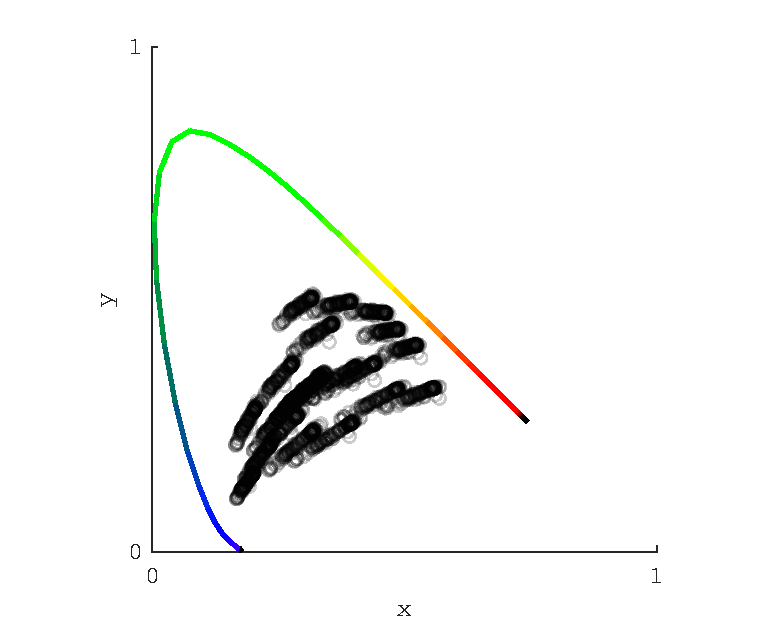
\includegraphics[max width=\textwidth]{figs/LitRev/ColorimetryDemo6.pdf}
\caption{A reproduction of Figure \ref{fig:1931}, but this time with the chromaticity co-ordinates for the 24 macbeth colour checker patches under a range of daylights, drawn from the Granada dataset \citep{hernandez-andres_color_2001} (further described in Section \ref{sec:coldata}).}
\label{fig:problem}
\end{figure}

In order to provide a representation of colour where the perceived colour remains constant across changes in illuminant (thus the term \emph{colour constancy}), the human visual system must find a way to solve this problem.

\subsubsection{Adaptation}

`Adaptation' is the general mechanism by which a finite range of sensitivity can be shifted within absolute sensitivity bounds. The benefit of having an adaptive system, as opposed to a fixed system, is that the sensitivity of the system to small changes is maximised, whilst maintaining a broad overall sensitivity, at the expense of being able to sense over the entire range at a single time-point. A visual demonstration of this is shown in Figure \ref{fig:Valeton} where it can be seen that that at a single level of adaptation (a single line) the range of intensity over which responses are generated is relatively small, but is extended through adaptation.

\begin{figure}[htbp]
\includegraphics[max width=\textwidth]{figs/LitRev/Valeton.png}
\caption{Cone flash response at different levels of adaptation in macaques, reproduced from \citet{valeton_light_1983}. On the left `DA' stands for dark-adapted, with the rising numbers for the other lines relating to rising adapting levels.}
\label{fig:Valeton}
\end{figure}

In an environment such as the terrestrial environment, there is a great range in the level of illumination, but this range is rarely existent contiguously; levels of illumination tend to be similar across a scene, and only change rather slowly over time. The notable exception, and thus where we notice the expense of having an adaptive visual system, comes when we enter or exit an environment where illumination is almost entirely excluded, such as a dark cave or below-decks of a boat. 

Where the process of adaptation responds to overall illumination levels, it is referred to as light adaptation and dark adaptation. Where the process of adaptation responds to the wavelength composition of light reaching the eye it is referred to as chromatic adaptation.

In a natural environment, a change in the wavelength composition of radiation reaching the eye from a specific object might be caused by changing weather or time of day, or by the physical movement of the object from one space to another (where different lighting exists in the two different spaces). Figure \ref{fig:SPDnorm} shows a set of measured daylight \glspl{SPD}, normalised by luminance, showing that the wavelength composition varies quite considerably, though in a relatively systematic fashion.

\begin{figure}[htbp]
\includegraphics[max width=\textwidth]{figs/LitRev/ColorimetryDemo7.pdf}
\caption{The \glspl{SPD} of a subset of the daylight measurements of \citet{hernandez-andres_color_2001} (further described in Section \ref{sec:coldata}), normalised by luminance.}
\label{fig:SPDnorm}
\end{figure}

\subsubsection{Mechanistic vs. Inferential}

In the literature there seems to be a long-running grapple between colour constancy and chromatic adaptation, with blurred boundaries and mixed definitions occurring frequently. \citet{brill_chromatic_1986} drive a wedge between the two concepts, but refute the traditional division that chromatic adaptation is the process and colour constancy is the ability, asserting that the two should be considered as separate processes, operating on different timescales and in different fashions.

\citet{hurlbert_computational_1998} divides computational models of colour constancy into two classes: \emph{sensory} and \emph{perceptual}, which broadly follow the low-level / high-level divide. `Sensory' models `could be achieved early in visual processing by adaptive scaling of the initial receptor responses'. `Perceptual' models `would necessarily occur at later stages of visual processing'.

Hurlbert [personal communication] notes that understanding the differing perspectives of researchers from different fields allows one to understand how the mixed use of these terms in the literature may have arisen: 

\begin{itquote}{}
The mixed use of the terms chromatic adaptation and colour constancy is largely explained by different usages in different fields. In \emph{colour science}, chromatic adaptation is often considered synonymous with colour constancy, as it is considered to be the only mechanism contributing to stabilising colour appearance under changes in illumination. In \emph{vision science}, colour constancy is generally defined as a perceptual phenomenon, and distinction is made between different contributory mechanisms at different levels (which \citet{hurlbert_computational_1998} attempts to define and onto which different proposed computational solutions are mapped).
\end{itquote}

Within vision science, the most common use of the term `chromatic adaptation' now seems to be to refer to low level adaptation, with \citet{brainard_color_2014} using the term `mechanistic' to refer to this type of transformation.

\begin{itquote}
Adaptation of this sort supports constancy to the extent that its overall effect is to stabilize the post-receptoral representation of the light reflected from objects across changes of illumination (as well as other contextual changes).
\end{itquote}

The term `colour constancy', by contrast, is used to refer to higher level inference-based processes, which occur at faster timescales than are possible by adaptation alone \citep{rinner_time_2000}. It seems likely that multiple processes work in tandem at multiple levels and timescales to achieve colour constancy \citep{hurlbert_colour_2007}.



\subsubsection{Von Kries Adaptation}

The conceptually simplest model of chromatic adaptation, and the forefather of many other models, is that referred to as Von Kries adaptation.

Johannes von Kries was one of the first to deeply consider chromatic adaptation, and appears to have understood it as a problem of sensory adaptation. In his formative series of papers, available in translation \citep{von_kries_beitrag_1970}, he laid out how the study of chromatic adaptation could be divided into two broad and complementary aims. 

The first referred to the systematic representation of the transforms in sensation caused by specific adaptations, such that \textit{``for any light mixture stimulating the readapted part [of the retina], another light mixture is specified that stimulates the same sensation in a normally adapted part \dots The purpose of this study would be solved completely if a general rule could be obtained for the effects of all possible adaptions.''} The search for `corresponding colours' (pairs of colours which match under asymmetric adaptation states), and for suitable systems to predict the appearance of colours in all situations, fall within this category of exploration. Out of this aim grew the study of \glspl{CAT}, where the search for an algorithm which would mathematically predict the locations in colour space of corresponding colours has been the fundamental goal \citep{cie_tc_1-52_cie_2004}.

Von Kries suggested that the second categorical aim of chromatic adaptation research ought to be to discover `how the adaptation is produced by exposure to any particular color, continued over an extended period of time.' 

Von Kries' distinction carves a divide between the study of the mechanisms of chromatic adaptation, and the effects of chromatic adaptation. It would be unreasonable to think of these areas of study as unrelated, but it seems reasonable to recognise their separability. 

%In the same set series of papers, von Kries laid out his understanding of chromatic adaptation, in terms of both how corresponding colours might be calculated, and how one might consider the underlying mechanisms which allow for colour constancy to operate. Here I shall abridge some of his writings to present the most salient insights, and attempt to explain what is meant by a `von Kries transform' in modern parlance.

Von Kries noted that `light mixtures that appear matched to the white-adapted eye always remain matched to the eye when it is adapted in any other manner.' This is known to be only partly true; if referring to photopic vision solely (where rods are bleached and cones provide the basis for vision). The implication of this statement is that the spectral sensitivities of the cone cells do not change as a result of chromatic adaptation. If they were to change in some way, then distinct mixtures of light which match in one adaptive state might fail to match under a different state. Von Kries referred to this idea as the `persistence rule.'

The second rule which von Kries presents is referred to as the `theorem of proportionality'. This theorem claims that when two pairs of corresponding colours (colours A and B under illuminant 1, and colours C and D under illuminant 2) are additively combined (A with B, and C with D), the resulting colours will also be corresponding colours. It follows from the von Kries' theorem of proportionality that increasing or decreasing the luminance of corresponding stimuli shouldn't void their equality, though of course this statement relies even more heavily on the caveat that this should only be assumed for photopic vision.

Von Kries goes on to suggest that it also follows that, if considered in combination with Grassmann's law \citep{grassmann_zur_1853}, the conversion of any arbitrary light by exposure to conditions causing a specific chromatic adaptation can be known if the nature of three other conversions are known. This relies on it being possible to consider any light as a linear combination of three others, and for the mechanism of chromatic adaptation to depend solely on the fatiguing of three independent systems.

Von Kries' assertions may be mathematically described as:

\begin{subequations}
\begin{align}
L_{a}&=K_{L}L \\
M_{a}&=K_{M}M \\
S_{a}&=K_{S}S
\end{align}
\end{subequations}

where $L$, $M$ and $S$ represent the cone group responses; $K_{L}$, $K_{M}$ and $K_{S}$ represent distinct scalars and $L_{a}$, $M_{a}$ and $S_{a}$ represent the post adaptation cone group responses\footnote{This specific notation is taken from \citet[p. 183]{fairchild_color_2013}.}. In terms of what might set these scalars, or gain values, von Kries suggested that: 

\begin{itquote}{von_kries_beitrag_1970}
the organ of vision becomes less effective for that kind or for that part of its performance which is demanded from it for an extended period of time, whereas it becomes more effective for the activity which is, in a sense, opposed to that. This can be conceived in the sense that the individual components present in the organ of vision are completely independent of one another and each is fatigued or adapted exclusively according to its own function.
\end{itquote}

Many interpretations have been made of this statement, and a corresponding number of nominations for methods by which to calculate values of $K$ have been proposed. The most frequently considered methods are those referred to as \acrfull{GW} (where the reciprocal of the mean response across a scene is used) and \acrfull{BiW} (where the reciprocal of the brightest point in the scene is used). \citet{finlayson_shades_2004} showed that these two variants can be considered as part of a single framework (Minkowski norm), and that other members of this family of algorithms provide benefits over \gls{GW} and \gls{BiW}.

Von Kries' thoughts have inspired many decades of research into \glspl{CAT}, which are a vital part of modern colour appearance models and other colour science computations, such as colour rendering index calculations. This relatively simple concept has remained relevant, as noted by \citet[p. 182]{fairchild_color_2013} who reproduces this quote:

\begin{citequote}{von_kries_beitrag_1970}
If some day it becomes possible to distinguish in an objective way the
various effects of light by direct observation of the retina, people will perhaps
recall with pitying smiles the efforts of previous decades which
undertook to seek an understanding of the same phenomena by such
lengthy detours.
\end{citequote}

followed by the comment:

\begin{citequote}{fairchild_color_2013}
Over eleven decades later, there is no one looking back at von Kries’ work
with a “pitying smile.” Rather, many are looking back at his work with
astonishment at how well it has withstood the test of time.
\end{citequote}

\subsubsection{Retinex}

Considered in the context on von Kries' work, the Retinex model of Land et al. \citep{land_retinex_1964,land_lightness_1971,land_recent_1983,land_recent_1986,mccann_quantitative_1976} might be described as `Von Kries adaptation with spatial considerations' but I imagine such a statement would have rather riled the often bombastic sounding Land. It appears to have been Land's understanding that the Retinex model was not a model of chromatic adaptation, but rather a model to usurp and do away with the very concept of chromatic adaptation (Land's papers on the subject \citep{land_retinex_1964,land_lightness_1971,land_recent_1983,land_recent_1986} do not once use the term `chromatic adaptation', nor is the work of von Kries ever explicitly referred to). 

Land was fond of picking apart Newton's statements regarding colour; particularly that the perception of colour was the result of an objects' `excess and predominance in the [spectra of the] reflected light' \citep{newton_opticks_1704}. Land asserted that rather than work from the premise that the visual system was correcting an absolute record of the world, by normalising it to account for the ambient light source, one should instead consider visual input only as a relative record, where each element within a scene only takes on properties by comparison with the other elements of the scene. 

He suggested for consideration the idea of the human visual system recording three separate lightness images, each representing the recording from a different band of receptors, where each element within each image is scaled against the brightest element in each specific image. Retinex theory also provides an interesting algorithm for discounting not only coloured illumination but illumination which varies across the visual field.

However, \citet{barnard_practical_1999} points out that the various versions of the Retinex algorithm simplify to versions of the Von Kries adaptation, and \citet{brainard_analysis_1986} found that `the algorithm is too sensitive to changes in the color of nearby objects to serve as an adequate model of human color constancy'. In addition, it has been found to be computationally difficult to implement, with no clear way in which it could be biologically implemented (though see \citet{hurlbert_formal_1986}).

The work of Land et al. has spurred a great deal of progress in the world of digital imaging, where the term `computational colour constancy' is used. The number of distinct algorithms increases at a rate which seems to always accelerate, and I shall not review them all here, though I shall point to valuable overview papers:  \citet{hordley_reevaluation_2006, gijsenij_computational_2011, hurlbert_computational_1998}.

\subsubsection{Linear models}

If we extend the common interpretation of colour constancy (that colours should remain constant), to a stricter case where we actively try to recover the \glspl{SRF} of surfaces, simple Von Kries-type transformations no longer suffice. \citet{maloney_physics-based_2001} and \citet{yang_illuminant_2001} discuss what they term the `RGB heuristic'. Simply put - this is the commonly held assumption that a set of cone catches under one illuminant will be related to a second set of cone catches under another by a transformation which can be fully described by the chromaticities of the illuminants. As \citet{maloney_physics-based_2001} says `there is no \emph{mathematical} reason to expect [this] to hold, even approximately'. This can be considered from the perspective of colour rendering; it is known that objects which are metamers under one illuminant might not be under another. This renders simple models of colour constancy ineffective. \citet{foster_frequency_2006} quantified the frequency of metamerism in real scenes and found it to be `sufficiently large to affect visual inferences about material identity'.

For this stricter definition of colour constancy Maloney et al. \citep{maloney_computational_1984, maloney_color_1986} propose a method which makes use of discrete linear models, whereby the set of real \glspl{SRF} and real \glspl{SPD} are approximated by a small number of fixed basis functions. 

\citet{maloney_color_1986} find that `with three classes of photoreceptors, we can exactly recover surface reflectances drawn from a fixed model of surface reflectance with at most two degrees of freedom'. \citet{maloney_computational_1984} showed that this generalised such that with $n$ classes of photoreceptors, \glspl{SRF} could be reconstructed for surfaces drawn from models with $n-1$ degrees of freedom, so long as there were not more than $n$ degrees of freedom in the illumination model, and so long as the minimum complexity condition was met (there were enough surfaces visible).

Despite its mathematical elegance, quantitative analysis of this algorithm showed that its performance was poor \cite{brainard_bayesian_1994, finlayson_color_1995}, which is not surprising considering that natural surface \glspl{SRF} generally require more than two basis functions for accurate reconstruction.

\bigskip

There are many further ideas, theories, and concepts relating to colour constancy and chromatic adaptation which are beyond the scope of this chapter, but that the reader may find of interest: gamut mapping algorithms \citep{forsyth_colour_1990,forsyth_novel_1990,forsyth_colour_1989,finlayson_color_1996}, bayesian colour constancy \citep{finlayson_color_2001, brainard_bayesian_2006,gazzaniga_bayesian_2009, brainard_bayesian_1994,gehler_bayesian_2008} and specular-reflectance-based algorithms \citep{mollon_monge_2006, morimoto_discrimination_2018,hurlbert_computational_1998}.

%% Removed stuff ---------------------------------


%Colour constancy refers to the stable perception of object colour appearance, in spite of a change in illumination which would cause a change in the nature of the stimuli reaching an observer\footnote{The terms `chromatic adaptation' and `colour constancy' are often used interchangeably; within this thesis I shall use `chromatic adaptation' to refer to an adaptive mechanism, and `colour constancy' as the ability possessed by an organism. For a discussion of the distinction of chromatic adaptation and colour constancy see \citet{brill_chromatic_1986}}. This objective change in stimuli seems to be effectively but not completely discounted by the human visual system; in order to maintain a stable perception of object appearance. 

%If however, one asked an observer whether the \emph{appearance} of an object has changed between the two conditions, the observer would generally say that it has. To some extent, we seem to have access to both the `raw input signals' and some estimate of the underlying \gls{SRF}.


%It is the popular understanding that when the illumination changes, the colour of an object (to use the term `colour' in its vernacular form, as representing an object attribute) does not change. This understanding holds true for all but the most extreme artificial illuminations, such as very narrow-band illuminantion. 


% \begin{figure}[htbp]
% \includegraphics[max width=\textwidth]{figs/LitRev/fosterflowers.png}
% \caption{A single scene under two illuminants (\Gls{CCT} = 4000k and 25000K), reproduced from \citet{foster_color_2011}.}
% \label{fig:fosterflowers}
% \end{figure}

% \begin{figure}[htbp]
% \includegraphics[max width=\textwidth]{figs/LitRev/greyballs.png}
% \caption{Reproduced from \citet{nascimento_spatial_2014}. Original figure caption: ``The color rendition on the left shows the scene with six embedded probe spheres indicated by numbers. The dot plot [on the right] shows the distribution of the CCTs of the local illumination at the 17 sample points on each of the spheres.''}
% \label{fig:greyballs}
% \end{figure}

%Figure \ref{fig:greyballs} gives an indication of the extent to which an object (or more precisely in this case, a group of nominally identical objects) can have varying colorimetric attributes across relatively minor spatial variation. 
%KC: This reads oddly to me, as it's more the illuminance that's varying than the object (if I've understood?).  I'd rephrase this.

% \begin{figure}[htbp]
% \includegraphics[max width=\textwidth]{figs/LitRev/X.png}
% \caption{\hl{Figure showing variation over time.}}
% \label{fig:X}
% \end{figure}

% Figure \ref{fig:fosterflowers} shows a single scene under illumination of two different \glspl{CCT}. The appearance of the object under the two illuminants is likely to have remained somewhat stable to an observer within the real scene, with observers choosing similar colour names for the object under each condition\footnote{Of course the appearance here, with these two images side-by-side, highlights the differences between the two conditions, and shows that under a single state of adaptation there is a clear distinction.}. 


% \subsubsection{Can chromatic adaptation fully account for colour constancy?}

% It may at first appear as though chromatic adaptation may be able to fully account for colour constancy

% RGB heuristic
% yes - cornsweet
% mechanistic vs inferential


% A similar level of variation occurs across time, for example as the sun passes behind a cloud.

% And so we have the central problem of colour constancy and chromatic adaptation: objects of which we have stable colour perceptions are able to be variant in both radiometric and colorimetric attributes without losing their apparent stability. The study of colour constancy aims to answer many questions which revolve around this central conundrum.

% Traditionally %(pre-1986, when \citet{arend_simultaneous_1986} performed what \citet{foster_color_2011} refers to as `the first systematic behavioral experiments' on color constancy) 
% there have existed two stances regards the nature of colour constancy; one held that it was enabled by adaptation of the sensory system, and the other that it was the result of unconscious inference. %KC: citation required
% It is my understanding that whilst great progress has been made in the intervening three decades, this is still a central question, although it appears to be widely accepted that the two frameworks might be complementary rather than mutually exclusive. %KC: citation required

%The best justification for their separation is perhaps that success in their study might serve different aims. 
%The first, the prediction of colour appearance, serves to further the utility of colour science, in particular colour appearance modelling, and the other systems which rely upon colour appearance modelling, such as colour difference formulation. 
%The second is best considered a vision science problem, concerned as it is with the function of the human visual organ, and advancement might endow us with an extension in our understanding of the human body. This in turn would have benefit in multiple areas, including feeding back to the prior aim, for once we understand the underlying mechanics we stand a much better chance of creating robust predictors of colour appearance. 
%Of particular interest to this author, understanding the underlying mechanisms of colour constancy should allow for a more intelligent design of lighting for the spaces which we inhabit, considering that artificial lighting need only resemble natural lighting to the extent that the visual system treats it as similar enough. Creating a colorimetric match to a specific spectra such as D65 is relatively easy, but until chromatic adaptation is more thoroughly understood it is not necessarily entirely clear what the appearance of such a match, or objects illuminated by it, might be. 

%The investigation of \glspl{CAT} generally occurs through the fitting of algorithms to data of corresponding colours, collected in varying manners, such that corresponding colours might be predicted for specific situations. The principal divides between the types of \gls{CAT} tend to hinge upon the method used to collect the data. \citet{nayatani_development_2006} divides the set as those derived from chromatic adaptation theory and those derived from fitting to experimental data, whereas Luo44 makes the divide between those studies based on aperture based experimental procedures and non-aperture based experimental procedures (which generally incorporate more complex, and therefore arguably more realistic, stimuli). Both parties use the terms `CAT Type I/II' to refer to these distinctions, but it is not entirely clear whether their distinctions are complementary. 

% This duality %get rid of this bollocks
% is mirrored by Foster37 in his discussion of the experimental methods employed in colour constancy research where he describes fundamental differences between those experiments which probe chromatic adaptation by asking observers to make `paper matches' (make it look like these two patches were cut from the same sheet of paper) and h/s/b matches (where observers are asked to match appearance in a non-relational manner, that is to match the qualia of a stimuli). This duality occurs again in Foster's37 comparison of relational and non-relational colour constancy, where relational refers to the maintaining of colour relationships in a scene and non-relational again refers to abstracted stimuli qualia). It is my suspicion that all of these disparate dualities are representations of the fundamental duality considered at the beginning of this chapter; that of a distinction between sensory adaptation and inferential computation.

\subsection{Experimental Methods for Colour Constancy Research}

\begin{citequote}{hurlbert_colour_2007}
\emph{How is colour constancy measured?} With difficulty.
\end{citequote}


\hl{A large range of experimental methods have been used to investigate the problem of colour constancy \dots} % partly because different experimenters were approaching the problem from different angles aiming to accomplish subtly separate goals.
% Those approaching from a mathematical angle (perhaps with the mind-set `if we find the algorithm which predicts corresponding colours a- this is very useful for industry and b- we can then work backwards to explain how human colour constancy may occur') are concerned primarily with producing chromatic adaptation transforms.
% Those approaching colour constancy with a basic interest in the physiology and general function of colour constancy have adopted/created a rather wider set of experimental techniques, owing to the fact that this direction of study is much less well defined than the former, and is at a more exploratory stage of its development.
% The \gls{CIE} TC 1-52 report (\gls{CIE} 160:200442) includes an interesting note on the distinction between these two broad approaches; an appendix discusses the reasons why a concerted recommendation was not reached by the group lists the principal factor being a distinction between perspectives as described above. 
% \gls{CIE} TC 1-5242 and Luo44 provide a comprehensive overview of the different methods which have been used by the CAT group:
% 1.	Haploscopic matching
% 2.	Local Adaptation Matching
% 3.	Memory Matching
% 4.	Magnitude Estimation
% Haploscopic Matching is the most common technique in this field, and the term refers to experiments which differentially adapt the two eyes and allow an observer to vary attributes of the stimulus presented to one eye such that it in some way matches the attributes of a fixed stimulus shown to another eye. Whilst this is in many ways unnatural, the benefits are that an experiment can be set up so that there is no time interference (the presentations are simultaneous, so memory effects are avoided) and that high precision of match is relatively easily achieved. As assumption is made that the adaptation of each eye is independent.
 
% Figure 11 From42.
% Local Adaptation Matching can be considered as a variation of haploscopic matching where instead of differing adaptational stimuli being presented to each eye, differing adaptational stimuli are presented to different parts of the same eye (spatially distinct areas of the same retina). The assumption here is that there is minimal intra-retinal interaction. MacAdam's 1956 study49 epitomises this technique. This experimental technique requires that observers minimise eye movement, in order to maintain spatially distinct adaptation.
% Memory Matching has traditionally been performed by training observers to communicate colour sensation through the munsell system notation50,51, and then asking observers adapted to different ambient lighting to describe set real objects using such notation. This technique is not much used due to many limitations and confounding factors. Luo44 details the limitations  of this experimental technique succinctly: `a substantial training period being required, complicated procedures for data analysis, lower precision than that of haploscopic technique, limited capacity for retaining information, and memory distortion.'
% Magnitude Estimation appears to be similar to memory matching, in that observers are requested to verbally describe an object whilst in an ambient adapting field. The distinction is that the observers are requested to communicate their perceptions using the perceptually meaningful attributes of hue, saturation and brightness, and as such results can be easily integrated into colour appearance models. Recent experiments52,53,54,55,56,57 collected data which was used to create CIECAM97s.
% Away from the development of CATs, a subtly different set of experimental techniques has been developed with which to probe the operation of colour constancy. An admirable overview is provided by Foster37:
% 1.	Asymmetric Matching
% 2.	Colour Naming
% 3.	Achromatic Adjustment
% 4.	Discriminating Illuminant Changes from Reflectance Changes
% Asymmetric matching is in many ways synonymous to the haploscopic matching described above and by in \gls{CIE} 160:200442, in that it describes an experimental set-up whereby one stimuli is compared with another, generally where each stimuli exists within a distinct adapting field and attributes of one stimuli can be either adjusted or responded to by an observer. The term asymmetric matching might be thought to be inclusive of a wider range of experimental set-ups, where haploscopic (Greek roots: haploieides, single and skopeo, to view) is necessarily concerned with each individual eye receiving distinct input. Asymmetric matching may refer to experiments where stimuli are viewed simultaneously, successively, or in an alternating fashion, binocularly or haploscopically.
% Colour Naming is a technique employed with the aim being a more natural task than  asymmetric matching, and removing some of the `instruction effects' probed by Arend and Reeves40. Foster argues37 that colour naming represents a task apt to measure colour constancy more directly, as opposed to the `relational colour constancy' often studied in asymmetric matching experiments, since it concerns identification rather than equivalence. One clear benefit seems to be that the observer needn't be aware of the equivalence; it is expected that in such experiments there will be only one stimulus, perhaps with a temporally variant adapting field. An observer is simply asked to name colours, and this should theoretically result in a measure of adaptational colour constancy as opposed to inferential colour constancy, so long as the stimuli is suitably abstract . Colour names may be of a fixed set, or an observer may be given free choice. Analysis of results can employ a naming centroid based approach or a boundary focused approach. Speigle and Brainard58 proposed a novel approach combining magnitude estimation and colour naming with the aim to improve precision of response.
% Achromatic Adjustment experiments ask an observer to in some way set a stimulus to a neutral achromatic tone, on the assumption that the internal grey point of an observer shifts in response to different adapting fields. These adjustments are generally easy for an observer to make, but the extrapolation of the results makes various assumptions about conceptual colour space and the nature of achromacy. Experiments are easily confounded by complex or real stimuli where there exists a close-to-neutral object in the scene which could consciously or unconsciously be used as a reference.
% Discriminating illuminant changes from reflectance changes provides a key way to examine colour constancy in an operational manner. Following the assumption that chromatic adaptation allows an observer to discount the illuminant in some manner, an experimental set up where observers are requested to distinguish between an illuminant change and a reflectance change represents a situation which very closely mirrors the natural process of colour constancy. This experimental technique is well placed to examine whether or not colour constancy in this form is active and efficient, but it provides little way of probing the underlying mechanisms of colour constancy.

% %recent advances in colour constancy?
% % using more realistic stimuli
% % the grey edges algo
% % the comparison of grey edge and grey world/bright is white

\subsection{Intrinsically Photosensitive Retinal Ganglion Cells (ipRGCs)}

\textit{A recent review by \citet{spitschan_melanopsin_2019} provides an overview of this rapidly progressing research area.}

\bigskip

Retinal rod and cone cells (of three types, l/m/s) are well established as the primary receptors for human vision, and their connections and properties are relatively well understood. Two distinct signalling pathways originate from the retina, one which is associated with image formation and the other which is considered to be \gls{NIF}, and which influences systems such as circadian rhythm entrainment, pupillary reflex and melatonin release. It was originally thought that rods and cones were the sole inputs to both of these pathways\citep{hankins_melanopsin_2008}.

\Glspl{RGC} combine signals from groups of cones and rods and relay these signals via the optic nerve to the lateral geniculate nucleus, which in turn processes and relays them further to the cortex for additional processing, allowing for classical vision of objects, movement and colour. \Glspl{ipRGC} are a sub-class of retinal ganglion cells, which in addition to combining and relaying signals exhibit some intrinsic photosensitivity of their own. 

This intrinsic photosenstivity was only confirmed recently\citep{qiu_induction_2005} relative to our knowledge of other retinal cell types, following a search for a retinal cell type or combination of cell types which would fit the spectral sensitivity properties found to influence entraining the circadian rhythm in humans and other animals\citep{brainard_human_2001,brainard_action_2001}, which was dissimilar to all of the spectral sensitivities of the cell classes known at the time.

Additionally, it was found that animals and humans with no functioning cones or rods were still able to have a correctly functioning circadian system\citep{freedman_regulation_1999,zaidi_short-wavelength_2007}, further suggesting that that the circadian rhythm was influenced by a novel receptor with a distinct photoreceptor. It is now believed to be these cells which provide input to the second of the signalling pathways originating in the retina, that which controls the \gls{NIF} response to illumination.

\Glspl{ipRGC} were found to express a photopigment fitting such attributes, named melanopsin. The spectral sensitivity of melanopsin peaks around 480nm\citep{qiu_induction_2005,hankins_primary_2002,dacey_melanopsin-expressing_2005,peirson_melanopsin_2006,bailes_human_2013} which places it between the s-cone (cyanolabe photopsin) and rod cell (rhodopic rhodopsin) peak spectral sensitivities%, see Figure \ref{fig:specsens}
. In humans, pre-receptoral filtering leads to a functional peak sensitivity of closer to 490nm\citep{cie_cie_2015-1}. There is uncertainty regarding the potential bistable nature of melanopsin, and whether this would have a functional effect on the spectral sensitivity of melanopsin\citep{cie_cie_2015-1,mure_melanopsin_2009,rollag_does_2008}.

\Glspl{ipRGC} are sparse in the retina; discounting input from other cell types, they operate at a much lower resolution than as would be required for meaningful spatial vision. They also operate much more slowly compared to other cell types, taking several seconds to respond, but are able to sustain a response in contrast to other retinal cell types which are able to respond quickly but only for short periods.

It has been proposed that \glspl{ipRGC} may allow an observer to sense a level of absolute irradiance\citep{brown_melanopsin_2010}. 

\subsubsection{The image-forming role of ipRGCs}

In recent years there has been a large number of publications examining the role of melanopsin outside of \gls{NIF} vision.

Spatial:
\cite{ecker_melanopsin-expressing_2010}
\cite{spitschan_vision_2017}
\cite{mouland_responses_2017}
\cite{allen_melanopsin_2017}
\cite{allen_form_2019}

Colour:
\cite{cao_evidence_2018}
\cite{spitschan_human_2017-1}
\cite{zele_melanopsin_2018}

\section{Museum Lighting}

\bigskip

\begin{quote}
`Museums and art galleries collect, preserve, and display natural artifacts and/or examples of human achievement and analyze their impact on the world and the universe around us. Effective exhibit lighting must balance exhibition and conservation needs and enrich the museum experience.'
\end{quote}

\begin{flushright}IES RP-30-96 Museum and Art Gallery Lighting: \\A Recommended Practice \citep{ies_ies_1996}\end{flushright}

\bigskip

Lighting in museums is required to satisfy multiple criteria; perhaps the least contestable requirement being that the lighting illuminate objects such that they are suitably visible to museum visitors. Also of utmost importance in most museum settings is that the lighting does not have an unreasonably damaging effect upon the objects or environment, be this through direct photodegradation or as a result of heat transfer. Further to these requirements, an increased or optimal visual quality is generally desirable, although what this represents or how to achieve it is generally ambiguous.

In sweeping terms, all electromagnetic radiation (visible and non-visible) damages objects, and more radiation damages objects proportionally moreso. Thus the question becomes: \emph{how little light can we use to illuminate objects such that they're visible to the extent required?} The inverse form, sometimes used on the assumption that more light always represents an increase in observer satisfaction/pleasure is: \emph{`how much light can we use so that only $x$ damage occurs over $y$ time'}. 

Industry guidance documents provide advice on how to manage lighting to best address the above requirements and many other additional specific requirements through the recommendation of procedure and provision of target figures for quantitative variables. \Gls{UV} radiation, being of no visual benefit but having potential to harm, is now excluded from gallery spaces as an industry standard.

\subsection{Damage functions} \label{sec:DamageIndex}

\textit{The key reference on this subject is CIE 157:2004 \citep{cie_cie_2004}, and valuable talks on the subject were given at the recent Museum Lighting Symposium \& Workshops\citep{pokorska_book_2017} (which the author helped to organise), and have been made freely available online\footnote{See in particular the talks by David Saunders (\url{https://www.youtube.com/watch?v=H4d0qH0IBcI&t}) and Stefan Michalski (\url{https://www.youtube.com/watch?v=XUY9biLQqlw})}.}.

\bigskip

In heritage science `damage functions' are ``functions of unacceptable change, dependent on agents of change''\citep{strlic_damage_2013}. The goal of damage functions in heritage lighting engineering is to give a quantitative means by which to predict the amount of damage caused to a prototypical object by a given light source, and to assist in limiting such damage. They generally follow the logic that radiation of lower wavelength is likely to cause more damage to objects.

\citet{harrison_report_1953} is generally acknowledged as the first to suggest such a function, but he himself acknowledges that it had ``long been established that the shorter the wavelength (visible yellow, green, blue, violet and invisible UV being progressively shorter) the more photochemically potent will be such radiant energy, provided such energy is actually absorbed''. \citet[p.9]{harrison_report_1953} defined the `radiation hazard associated with a light source' as:

\begin{equation}
    \sum_{0}^{\infty} \mathrm{H}_{\lambda} \mathrm{D}_{\lambda} \Delta \lambda / \sum_{0}^{\infty} \mathrm{H}_{\lambda} \overline{\mathrm{y}}_{\lambda} \Delta \lambda
    \label{eq:Harrison}
\end{equation}

where $\mathrm{H}_{\lambda}$ is the spectral irradiance, $\mathrm{D}_{\lambda}$ is the `Relative Damage Factor' (which is extrapolated from the data collected shortly prior to Harrison's own report by the National Bureau of Standards \citep{national_bureau_of_standards_preservation_1951}, and shown in Figure \ref{fig:Harrison}), and $\overline{\mathrm{y}}_{\lambda}$ is the CIE 1924 photopic $V_{\lambda}$ luminosity function. The resulting value would describe the amount of damage expected from a light source, normalised by its luminance.

\begin{figure}[htbp]
\includegraphics[max width=\textwidth]{figs/LitRev/HarrisonInd.pdf}
\caption{Harrison's \citep{harrison_report_1953} damage function ($\mathrm{D}_{\lambda}$), and luminous efficacy ($\overline{\mathrm{y}}_{\lambda}$), alongside the Declaration of Independence data \citep{national_bureau_of_standards_preservation_1951} from which it was extrapolated (re-normalised to match scale).}
\label{fig:Harrison}
\end{figure}

\begin{figure}[htbp]
\includegraphics[max width=\textwidth]{figs/LitRev/Saunders.pdf}
\caption{Graph courtesy of David Saunders, presented at the Museum Lighting Symposium \& Workshops \citep[p.61]{pokorska_book_2017} showing the relationship between wavelength and the bonds which can be broken in various molecules, with `Wavelength (nm)' on the abscissa and `Bond energy (kJ/mol)' on the ordinate.}
\label{fig:Saunders}
\end{figure}

There has been extended scepticism about the utility of damage functions in general, with the argument being that no one damage function could represent the vast range and complexities of real materials. \citet[p. 178]{thomson_museum_1978} wrote that ``for more fugitive materials \dots the figure for visible radiation would be higher. On the other hand \dots the fastest dyes are probably affected only by UV. Thus it can be seen that no single figure can be given for damage versus wavelength''.

Criticism was aimed at this specific damage function due to it's derivation from such a small and minimally representative dataset - Harrison's data was `extended' from the 5 datapoints measured by the National Bureau of Standards \citep{national_bureau_of_standards_preservation_1951} in their investigations of how to best care for the Declaration of Independence\footnote{It is a curiosity that these minimal figures would not in fact have been much use to those planning the care for the declaration, since in the report it is noted that ``The deterioration of animal parchment is not as rapid as that of the low-grade paper for which the damage factors were determined''\citep{national_bureau_of_standards_preservation_1951}, and the Declaration of Independence is written on animal parchment.}, and was derived from the study of `low-grade paper', which cannot to said to represent the average museum item\footnote{Though \emph{no} material truly can!}.

CIE 157:2004 \citep{cie_cie_2004} notes that whilst Harrison's proposal failed to gain acceptance as the procedure for comparing the damage potential of different types of light sources, it did convince people of the ills of \gls{UV}, with the result that daylight was subsequently eliminated from many galleries.

Following \citet{cuttle_lighting_1988}, who noted that Harrison's damage function could be well fit by an inverted logarithmic function, with parameters controlling the slope and normalisation point of the function, CIE 157:2004 provided the following equation:

\begin{equation}
    s(\lambda)_{\mathrm{dm,rel}}=\exp [-b(\lambda-n)]
    \label{eq:damfac}
\end{equation}

where differing values of $b$ for 5 categories of item are provided (Table \ref{tab:b}), $n$ is the normalisation value (CIE 157:2004 uses a value of 300), and the $s(\lambda)_{\mathrm{dm,rel}}$ function is the estimated action spectrum for each category. $s(\lambda)_{\mathrm{dm,rel}}$ would be substituted into Equation \ref{eq:Harrison} for $\mathrm{D}_{\lambda}$. CIE 157:2004 also provides values of $H_{s,dm}$ which indicate the susceptibility of each group of materials to damage (where damage is considered as colour change%in $\Delta E_{\mathrm{ab}}^{\ast}$
).

\begin{table}[htbp]
\centering
\begin{tabular}{|c|l|l|l|}
\hline
Group & Samples & $H_{s,dm}$ (W h/m$^{2}$) & $b$ \\ \hline
a & Low-grade paper & 5 & 0.038 \\ \hline
b & Rag paper & 1200 & 0.0125 \\ \hline
c & Oil paints on canvas & 850 & 0.0115 \\ \hline
d & Textiles & 290 & 0.0100 \\ \hline
e & Water colours on rag paper & 175 & 0.0115 \\ \hline
\end{tabular}
\caption{Table reproduced from CIE 157:2004 \citep{cie_cie_2004}, showing the values for $H_{s,dm}$ and $b$ for various categories. Note: the source for this data is not particularly clear; it is listed as `The Berlin researchers', which is assumed to follow the references: \citet{krochmann_beleuchtung_1988,cie_cie_1991,hilbert_zur_1991}; none of which I have been able to access.}
\label{tab:b}
\end{table}

The more general criticism that damage functions will never be able to represent all museum objects is a valid concern, and can be well illustrated with the following logic: museums own objects of many different colours, different colours arise from different reflectance properties, different refelctance properties mean different wavelengths are absobed, and damage can only occur when radiation is absorbed. Thus it follows that one would expect two objects of different colours to have different damage functions. 

The classic study on how reflectance properties relate to damage is that of \citet{saunders_wavelength-dependent_1994}. They exposed a number of pigments to a range of wavelengths and measured the resulting damage. \citet{cuttle_control_1999} later replotted the data from this study (reproduced in Figure \ref{fig:Cuttle}), highlighting the apparent joint contributions of spectral reflectance and a general damage function to the individual damage functions. CIE 157:2004 notes however that this correspondence is not perfect or easily modellable, and that ``a workable system for characterising action spectra for colorants, including pigments and dyes, remains an unattained goal``. Recent studied have added new data (see esp. \citet{villmann_wavelength_2018}), and it is hoped that a general understanding may at some point be reached.

\begin{figure}[htbp]
\includegraphics[max width=\textwidth]{figs/LitRev/Cuttle.pdf}
\caption{Figure of \citet{cuttle_control_1999}, using data from \citet{saunders_wavelength-dependent_1994}, and reproduced here from CIE 157:2004 \citep{cie_cie_2004}.}
\label{fig:Cuttle}
\end{figure}

However, it is the opinion of this author that this argument is an exercise in artificial futility; whilst we may not be able to model the individual damage functions for every object in a museum, we may at least use one which has some bearing on the damage function, rather than the one which is implicitly used by museums currently - the CIE 1924 luminosity function ($\overline{\mathrm{y}}_{\lambda}$ of Figure \ref{fig:Harrison}), which relates to the sensitivity of the human eye rather than any type of object. \citet{cuttle_lighting_1988} puts it well: ``The argument, then, is not whether we have a [damage] function which is correct, but whether we can improve usefully upon the likely reliability of the present system''.
% See xxx

In the case where specific objects/pigments of interest can be identified, and their individual damage functions calculated, there is valuable recent research to draw on regarding methods for optimising light sources to minimise damage \citep{durmus_optimising_2017,durmus_colour_2015,durmus_optimising_2015,durmus_object_2017}.

With modern computation, and access to datasets, it becomes relatively easy to calculate a value of \Gls{DI}. Figure \ref{fig:Houser} shows the results for such computations for 401 illuminants and light sources (as per Equation \ref{eq:Harrison}, using a damage factor computed as per Equation \ref{eq:damfac}, but further normalised such that Illuminant A has a reference value of 1)\footnote{The code to reproduce this is available from: \url{https://github.com/da5nsy/DamageIndex}}. It can be seen that whilst most illuminants cluster around 1 there is a broad range. It should be remembered that these illuminants would in no way indicate their relative damage index to an observer or a purchaser, unless one went to the effort to look up or measure the \gls{SPD} and compute the damage factor. A careful or careless choice in this respect could easily double or halve the amount of time an item could be exhibited before succumbing to terminal damage.

\begin{figure}[htbp]
\includegraphics[max width=\textwidth]{figs/LitRev/DI.pdf}
\caption{The values of $DI$ for the 401 illuminants used by \citet{houser_review_2013}, available via \gls{PTB} as `spd\_houser', normalised such that \gls{CIE} Illuminant A receives a reference value of 1.}
\label{fig:Houser}
\end{figure}

\subsection{Interviews with Museum Professionals} \label{sec:Interviews}

\textit{The following work has been published as \textbf{`How is museum lighting selected? An insight into current practice in UK museums'} \citep{garside_how_2017}. An overview is presented here, focusing on the elements relevant to the rest of the thesis, rather than as an independent chapter.}

\medskip

In order to gain an understanding of how museum professionals currently specify lighting, interviews were conducted with 12 museum professionals representing 10 UK based museums, galleries or historic property management groups, in spring of 2016. A small number of these professionals represented UK-wide groups, but the majority represented London based institutions.

The interviews were semi-structured around a set of questions composed by the author and their academic supervisors (reproduced in \citet{garside_how_2017}). The choice to conduct these interviews in a semi-structured format as opposed to a fully-structured one was based on the desire to allow unanticipated topics to enter the conversation, so as to limit the potential for important subjects to be neglected due to naivety of foresight. The conversational format of the interviews meant that the resulting data was qualitative rather than quantitative, which to an extent hinders comparison, but it was decided that the variety of job roles and institutional sizes, and the small sample size, already made quantitative comparison of limited meaningfulness for this investigation.

The interviewees were contacted through introductions from supervisors, personal connections, or cold emails. Almost all held conservation based roles (the exception being an `exhibitions manager') and noted that their principal responsibility regards lighting was controlling the safety of lighting regards its ability to cause damage to the objects held and displayed by their respective institutions. This generally involved monitoring and analysis of existing lighting systems and natural illumination, creating general guidance documents for the specification of lighting in their specific institutions and for loan items, and providing guidance and recommendations for the fitting out of new galleries or gallery refits. Few considered themselves directly responsible for the appearance of museum objects, considering this to be a creative decision outside of their remits. Future work considering the perspective of others involved in museum lighting, such as representatives from external lighting design companies, is required.

Whilst a small number considered themselves active in the area of lighting research, all interviewees were responsible for more conservation considerations aside from lighting, limiting the practicable level of specialisation. Many considered communication and dissemination a key part of their role, often noting they often found themselves in the position of needing to educate other teams within their institution on subjects including lighting. 

\begin{quote}
``This is not my science, my job is pulling it out and presenting it to others.''
\end{quote}

Asked what each considered to be `good lighting', responses included `safe', `invisible' (you don't notice it), and `lighting which is appropriate for your objects and your exhibition' (noting the variability of requirements dependent on the particular object(s) being presented). Asked to present a list or range of priorities, many focused on the safety requirements of lighting. The principal safety concern for lighting was that it fell below specific illuminance criteria, dependent on the assumed sensitivity category of the object in question. The specific target values were generally those provided by \citet{thomson_museum_1986} of 50lx for sensitive items and 200lx for less sensitive items (which are based on the visual preference work of \citet{loe_preferred_1982}).

Considering a scale of other priorities, following the requirement for appropriate lux levels, considerations included: limiting/excluding \gls{UV}, obtaining an acceptable \gls{CRI} value, and time and capital costs associating with fitting and maintenance. Energy efficiency was also a driver, but this did not seem to be a factor within technology category, rather it was noted that many institutions are switching to \gls{LED} because of increased efficiency, but that the difference in efficiency between one \gls{LED} type and another was negligible compared to the saving in contrast to lighting technology which \gls{LED} was replacing, which was often tungsten.

The range of roles played in the procurement of lighting varied amongst those interviewed. Whilst some created guidance documents which would then be passed on to estates teams and exhibition designers or lighting designers specifically, others had a much more hands-on role, testing specific lighting before installation or making recommendations on a case-by-case basis. It was noted that whilst relamping and retrofitting was generally handled by `in house' teams, where new galleries or large temporary exhibitions were created it was common for an external lighting design company to be contracted to perform the work. When asked whether recommendations were normally followed, the general reply was that recommendations for lux exposure and UV content were almost always followed, but other recommendations (such as for \gls{CRI} or \gls{CCT}) were more loosely interpreted. In many cases recommendations for \gls{CCT} were not made.

When asked about the tools used to make such recommendations and choices, responses included references to guidelines and reference sources (most often \citet{thomson_museum_1986}, though also \citet{druzik_guidelines_2012} and \citet{british_standards_institution_pas_2012}), references to specific units such as `lux' used in tandem with recommendations from guidelines such as above, indices such as the \gls{CIE} general colour rendering index R$_a$ (referred ubiquitously to as `\gls{CRI}' by interviewees) and notes of specific conferences which were attended in order to stay up to date with the research on the subject. There was a general feeling that the current climate was one of swift technological change in lighting, which created an increased difficulty in staying up to date with developments. It was noted that attending conferences and industry workshops were very beneficial in assisting professionals to stay up to date. 

\begin{quote}
`   Things are moving so quickly that to rely on books which have taken two years to produce [does not suffice, because] things have moved on. Books (plus journals) used to be the main reference. Now things are moving at such a rapid pace.''
\end{quote}

A range of techniques were used to qualify whether specific lighting was `safe' or not. The most common practical technique was spot metering of lux values incident on specific objects, and selective dimming to drop incident lighting to the desired lux level in response to this. Some larger institutions with access to microfading equipment were able to use this in the determination of sensitivity of specific objects. One interviewee provided details of a spectral power distribution based method for considering the safety specifically of phosphor based \gls{LED} illumination, whereby the height of the blue peak was compared to the height of the peak of the broader peak above 500nm, and if the former was more than three times the height of the latter, that lighting was singled out as potentially not safe. Other interviewees had heard of this criteria, and some used it as a rough guide, but one remarked that it was `fairly arbitrary'. One of the most succinct and perhaps astute responses was ``what is `safe'?''. One interviewee referred to the website of \citet{padfield_relative_2012} where considerations for the `RE\%' (`relative spectral sensitivity normalised exposure values'), using the damage functions described by \citet{aydinli_deterioration_1990} are used.

The interviewees generally did not consider characteristics of the displayed objects such as geometry of illumination, broadly considering this to be the remit of a lighting designer or exhibition designer rather than a conservator.

One of the most interesting, and perhaps surprising findings was the ubiquity of visual testing of lighting, generally performed prior to any large installation. For relamping, manufacturer supplied attribute values were generally relied upon as this required less time/effort and was cheaper. The most common procedure for new installations seemed to be for an informal and minimal visual test to occur before widespread installation. In a single case however, visual testing was actively avoided (on the basis that visual testing could not deliver meaningful insights where the aim was accurate rendering as opposed to visually pleasing rendering) and in another case large scale visual testing was performed, including many different types/brands of lamp and a large number of museum staff, and a final decision was made almost entirely on the results of this testing.

\Glspl{LED} are now used, at least in part, in all the institutions involved in this survey. In several they are the primary lighting technology but in a small number they are used sparingly, only in applications such as the lighting of text information panels. In one they are used in a particularly minimal fashion, although this was attributed to the fact that the museum is moving location in the near future and thus capital investments in building infrastructure were being avoided for the present time. There was no one specific brand or type which seemed to be ubiquitous across institutions, rather each institution appeared to have relationships with different manufacturers and suppliers.

Most interviewees were aware of warnings which had been issued and well publicised in the mainstream press \citep{lewis_smith_will_2013} regards the potential of \gls{LED} sources to be especially degrading for specific objects. Interviewees saw these warnings as controversial and likely unwarranted, and were confident that research had been conducted which cleared \Glspl{LED} of causing an unacceptable level of damage in comparison with alternative technologies. When asked how they might assess a light source for safety, most replied that safety was assessed solely through use of an illuminance meter and lux targets, not through analysis of the \gls{SPD} or any other lighting attribute. Those who did critically assess the \gls{SPD} generally used no specific tools to do so, focusing attention on the wavelength of the spectral emission peak.

\begin{quote}
``We never normally adjust the lighting type for a given artwork, we adjust the intensity''
\end{quote}

\begin{quote}
``For all lighting we measure the \gls{SPD}, and check it is reasonable''
\end{quote}

They key driver behind the adoption of \Glspl{LED} appears to be energy efficiency increases and energy use reductions, as required by institution-wide directives, or as part of applications for planning permission. Secondary to this consideration, benefits noted include: decreased maintenance costs from extended lifetime of products, and a lack of availability of traditional bulbs, sometimes due to specific legislation which has in effect phased out some traditional technologies. One element holding back some interviewees from further investment was a residual feeling that this new technology was not yet fully proven. Many pointed out that the claims made regards extended lifetime of \Glspl{LED} were yet to be proven in real world environments due to the relatively new nature of the technology. Some also noted the high costs associated with having to change the underlying lighting infrastructure, where retrofitting wasn't possible or appropriate. A final note on this section - some interviewees were unsure about the ability of \Glspl{LED} to remain colour stable over the long expected lifetime of the products.

Interviewees reported that visitors had not generally responded to any changes in lighting technology, and this was taken to mean that any switch to \gls{LED} had not been negatively received. It was inconclusive whether or not the technology was positively received however. This could be a meaningful avenue for future work. In terms of the professionals own opinions of \gls{LED} lighting, all seemed favourable, though it was unclear how much of this effect was caused by extraneous or related effects such as a placebo effect due to the excitement of new technology, or different chromaticities or brightnesses of replacement technologies.  

\begin{quote}
``I like what I've seen. The galleries where we have just \gls{LED} spots, I feel happier. I went to [another institution, with abundant \gls{LED} lighting], I really like the galleries where they had \gls{LED} lighting, and it was more of a gut feeling rather than something which I could put my finger on, but actually, it felt cleaner to me.''
\end{quote}

Whilst all interviewees were interested in the idea of making objects appear brighter whilst reducing the level of damage caused, the point was made that whilst spectral tuning might benefit a prototypical object, it will not necessarily benefit real objects in real environments. It was also noted that the use of lux in making decisions was particularly problematic here, where varying the location of a blue peak could easily increase the level of damage but reduce the lux value.
Most interviewees had a basic understanding of colour temperature, and a limited understanding of chromatic adaptation. The colour temperature of lighting was generally not seen as a conservation issue (though there were exceptions to this), and rather as a creative consideration. One interviewee noted that it was manipulated to great effect by external lighting designers in order to create specific effects or atmosphere.

The justification for \gls{CCT} specification values generally appears to stem from two routes. Firstly, from guidance documents such as those provided by The Getty and the Canadian Conservation Institute \citep{druzik_guidelines_2012}, and secondly from a desire to match existing lighting, either daylight or more commonly tungsten (at around 3000K). It was rarely considered as a means to control damage, or as a way to enhance visual appearance, by those interviewed. One interviewee referred to the work of \citet{kruithof_tubular_1941} and \citet{scuello_museum_2004,scuello_museum_2004-1} as justification for choosing low \gls{CCT} illumination similar to tungsten. No specific issues relating to colour temperature were raised by interviewees.

The interviewees were very interested in the subject of accurate representation, and almost all seemed to regard accurate object representation as a key priority. The figures for R$_a$ quoted in internal documents at each institution were either 80, 85 or 90, as a minimum figure. In one institution, an R$_w$ value was calculated for each proposed light source (the R value of the test colour sample with the colour shift of greatest magnitude, aka `worst') and a cut-off of 80 imposed. However, most interviewees seemed unsure of the practical relevance of R$_a$, with many considering it a rough guideline which would be considered secondarily to a visual inspection of lighting.

Those who were particularly interested in the subject gave the impression that whilst the subject was considered philosophically in great detail, the tool which was actually used to analyse the colour rendering of a light source was still generally just R$_a$. A few interviewees were aware of TM-30-15 \citep{color_metric_task_group_of_the_ies_ies_2015}, and whilst it was respected, it was questioned whether it represented a real improvement over R$_a$.
On the subject of lighting philosophy, the opinions encountered generally aligned with the mechanics of R$_a$. That is to say; given a choice between illuminating an object such that it was beautified, visually restored (to a previous condition) or simply presented as it would appear under daylight/tungsten illumination, most opted for the final option. Whilst there was clear interest in the other options, and other creative ways in which to consider colour rendering, it was generally believed that the role of the museum should be to represent objects in an un-biased manner, and thus a fidelity index was an appropriate tool for discussing a light source's colour rendering properties. In the case where specialist lighting was used to special effect, the opinion was noted that \textit{`you have to be very clear about what you are doing and why'} in order to maintain the reputation of the museum as an arena for honest and unbiased representation.

Generally, the interviewees believed that visitor requirements were being met (although there is often difficulty in defining exactly what visitor requirements actually are) and no specific tool or technology was proposed that would provide a clear benefit. Several interviewees mentioned that a way to improve the accessibility of colour rendering indices (in terms of the ease with which they could be understood and applied) would be appreciated.

No interviewees knew of recent surveys similar to the present one.

\subsection{Visitor Requirements of Museum Lighting}

The visitor requirements of museum lighting are varied and complex. The examination and definition of these requirements has been the subject of a small number of studies, principally by \citet{kesner_museum_1993-1} in the USA in the early nineteen-nineties \citep{kesner_museum_1993,kesner_exhibition_1992,kesner_current_1991,kesner_analysis_1997}. These studies were based on survey based self-reporting, and concluded that colour accuracy was the highest requirement and that `richness' of colour was the lowest priority\footnote{A cautious interpretation of these results is advised, considering that there were high average scores for each category}.

\begin{quote}
Artifact appearance, particularly clarity of artefact form and accuracy of artifact color, is the most important visitor need. Although visual impression, specifically acceptable gallery brightness and rich artefact color, is least important among the factors, it too rated highly important \citep{kesner_museum_1993-1}.
\end{quote}

Further studies, spurred by recent adoption of \gls{LED} technology have been completed, although with very limited and questionably scientific basis at the Field Museum \citep{myer_demonstration_2010}.

Additionally work has been completed which describes the results of a written survey of museum professionals on the subject of lighting specification, focusing on SSL (effectively \gls{LED}) adoption, and their justification for specifying specific lighting \citep{perrin_ssl_2014}. 979 people who had requested access to the guidelines document produced by some of the same authors \citep{druzik_guidelines_2012} were emailed with a request for participation. 46 (4.7\%) responded with a completed survey. Of those, 30\% are described as `international' which considering the base of the authors is in the USA we can assume as meaning `not based in the USA'. The survey was prepared as part of the USA government's GATEWAY program, and can be considered as a follow-up to work on recommendations for specification \citep{druzik_guidelines_2012}. 

\noindent
The headline results are as follows:
\begin{itemize}
    \item When the `success' of new \gls{LED} based lighting schemes was evaluated the public reaction was either neutral or positive in all cases \footnote{There appears to be an issue with the data for this question however, with the `no response' garnering 48\% of the responses and `favorable response' garnering 55\%\dots}
    \item The distribution of staff response was broadly similar: `no response'-17\%, `negative response'-3\%, `favorable response'-80\%.
    \item The results of two priority ranking questions\footnote{`Rank the following lighting goals' and `Please rank the following factors in your selection of lamps'} are broadly similar:
    \begin{itemize}
        \item First question: The first priority is identified as `limiting damage' with other priorities broadly equal.
        \item Second question: Joint first priorities are identified as `colour and spectral power distribution' and `damage potential' with others broadly similar (though dimming, input power and warranty lagging behind others)
    \end{itemize}
    \item 91\% of respondents reported using `\gls{CRI}' which is assumed to refer to \gls{CIE} R$_a$. 6\% state that they refer to other Ri values, and 20\% report using CQS (Color Quality Scale \citep{ohno_rationale_2010,davis_color_2010}).
    \item 60\% of respondents report that they consider \gls{CCT}.
\end{itemize} 

\subsection{Museum Lighting Specification Guidance Documents}

Following the interviews with the museum professionals, the five most referred-to museum lighting guidance documents were reviewed, and a summary is presented here.

\noindent
The guidelines chosen for review were:
\begin{itemize}
\item The Museum Environment \citep{thomson_museum_1986}
\item \gls{CIE} 157:2004 Control of Damage to Museum Objects by Optical Radiation \citep{cie_cie_2004}
\item Guidelines for Selecting Solid-State Lighting for Museums \citep{druzik_guidelines_2012}
\item SLL LG8: Lighting for museums and art galleries \citep{cibse_lighting_2015}
\item IES RP-30-96 Museum and Art Gallery Lighting: A Recommended Practice \citep{ies_ies_1996}\footnote{This has since been usurped by \citet{illuminating_engineering_society_ies_2017}.}.
\end{itemize}

\noindent
In summary:
\begin{itemize}
\item Recommended values were provided for:
\begin{itemize}
\item \emph{Lux}: various, dependent on sensitivity, generally based on figures from the study of visual preference by \citet{loe_preferred_1982}.
\item \emph{R$_a$}: various, most frequently \textgreater 80, with no experimental basis referenced.
\item \emph{\gls{CCT}}: various, based implicitly on \citet{kruithof_tubular_1941} or on such ideas found empirically.
\end{itemize}
\item Most also suggested visual inspection as a valid means of assessment.
\item There was often blurring between recommendations concerned with visual appearance and those concerned with conservation. 
\end{itemize}

\subsection{CCT in museums}

\acrfull{CCT} describes the chromaticity of a light source on a one dimensional axis roughly from blue to yellow, based on the apparent chromaticity of a black body radiator at differing temperatures. It is often described as an important variable in museum lighting but definite recommendations, in the rare cases that they are given, are generally based on very general rules that predict that damage potential will be decreased if \gls{CCT} is minimised \citep{cie_cie_2004}, nostalgia for the appearance of tungsten lighting or questionable research on human preference \citep{kruithof_tubular_1941,fotios_revised_2017}. Whilst some research appears to have found optimal \glspl{CCT} for viewing artwork \citep{nascimento_best_2014,pinto_correlated_2008,scuello_museum_2004,scuello_museum_2004-1, liu_cultural_2013} results often have large inter-observer variability, context dependency and it is not uncommon for the headline findings of separate studies to be in contradiction. 

Specifications often refer implicitly or explicitly to the findings of \citet{kruithof_tubular_1941}, who found that at lower levels of illumination, lower \glspl{CCT} were preferred, and that at higher levels of illumination higher \glspl{CCT} were preferred. Whilst this general trend seems to have anecdotal support, it is possible that there may be lighting-technology-based confounds, and recently researchers \citep{vienot_kruithofs_2009} (including a meta-study of multiple other examinations \citep{fotios_revised_2017}) found there to be no provable correlation between preference and colour temperature.

The \gls{CIE} however, published a report showing the varying the \gls{CCT} of museum lighting could have a clear impact on the potential damage undergone by museum objects \citep{cie_cie_2004}. 

\begin{figure}[hbtp]
\includegraphics[max width=\textwidth]{figs/LitRev/CIE2004.png} 
\caption{Figure reproduced from CIE 157:2004 \citep[p.16]{cie_cie_2004}, showing the relationship between \gls{CCT} and relative damage potential.}
\label{fig:CIE2004}
\end{figure}

This research relies heavily upon the applicability of damage functions to the specific materials in question. Many (my supervisors) think that damage functions are no good because they're too general, but I would be cautious about throwing the baby out with the bathwater.

\begin{enumerate}
    \item They're the best that we have.
    \item We need something with general applicability anyway - I don't see anyone providing tailored lighting for every object which exists.
    \item The physics checks out.
    \item They're definitely applicable to at least some objects.
\end{enumerate}

To verify the findings of the \gls{CIE}, to extend their findings to \glspl{LED}, and to provide code for others to do similar research or even test their own lights/materials, I wrote some code\footnote{\url{https://github.com/da5nsy/DamageIndex/blob/c7851e27ca1b0915013d8723db04704b49b4085e/CalcDI.m}} which would calculate a \gls{DI}. Then I used that code to compute a new version of the \gls{CIE} plot.

%\afterpage{\clearpage}
%\includepdf[pages=-,rotate=90, offset=75 -75]{figs/LitRev/CCTvsDI.pdf}
% \begin{figure}[t]
%     \caption{The \glspl{CCT} and \glspl{DI} of the \glspl{SPD} used by \citet{houser_review_2013} [provided via personal communication, but now partially available via \gls{PTB} as `spd\_houser'].}
%     \label{fig:CCTvsDI}
% \end{figure} 

\begin{fullpagefigure}
\figpdf[pages=-,rotate=90, offset=75 -75]{figs/LitRev/CCTvsDI.pdf}
\caption{The \glspl{CCT} and \glspl{DI} of the \glspl{SPD} used by \citet{houser_review_2013} [provided via personal communication, but now partially available via \gls{PTB} as `spd\_houser'].}
\label{fig:CCTvsDI}
\end{fullpagefigure}

The results of these computations show a clear relationship between \gls{CCT} and \gls{DI}. Considering that this is not currently taken advantage of in museum lighting, it seems as though there is a great potential for reducing damage whilst maintaining visitor visual satisfaction.

\subsection{Colour Rendering Indices in Museums}

Are fidelity indices suitable for museum use? 
The first chapter of Cuttle's book `Light for Art's Sake: Lighting for Artworks and Museum Displays'19 is titled `A philosophy for the presentation of art'. The choice of title here is apt but may surprise some readers, sounding more whimsical than might be expected of a serious subject attended by scientists and engineers. The reason it is so apt is because lighting is unavoidably a creative intervention (I owe this phrase to Katherine Curran); which is to say that there is no lighting which is truly impartial, and no lighting which is truly correct in the sense of being unequivocally superior to another. All lighting decisions require choices to be made, and whilst these choices can be wrapped up to appear as an optimization problem where proximity to a particular solution is the goal, the problem always rests on the bedrock of a philosophy based decision.

In the above mentioned chapter Cuttle lays out a total of seven distinct philosophical propositions, which he poses for consideration as approaches to museum lighting, some contradictory and some with the potential to overlap:

1.	`To make the artwork appear as it would have appeared to the artist at the time of its creation
2.	To ensure that no damage due to light exposure will occur
3.	To achieve the best possible appearance of the artwork
4.	To provide optimum conditions for viewing art
5.	To impart a sense of having seen `the real thing'
6.	To assist viewers to understand the displayed objects and their reason for being there
7.	For the lighting designer to establish a distinct and recognisable style'19 

These propositions refer to museum lighting holistically, considering all aspects of museum lighting, but can be readily focused on the problem of colour appearance specifically. Before we narrow our gaze however, it is worth briefly considering a wide view of lighting attributes which may aid in the realisation of `good quality' museum lighting. Consider Scott Rosenfeld's list of the five `controllable qualities' in museum lighting; `intensity, movement [temporal artefacts], angle [modelling, avoiding glare and reflections], distribution [ambient lighting vs. spot lighting], color'20.
Whilst Cuttle's propositions make for interesting discussions and enjoyable extended pondering, they are of limited assistance in the practical task of actually specifying lighting. Thankfully, a range of tools exist for the examination of the colour rendering properties of a light source, in the form of indices which aim to numerically describe an illumination's effect on colour appearance of the objects of which it is tasked with illuminating.

Traditionally, colour rendering indices aim to offer a standardized method for calculating the colour differences induced by the substitution of a reference illuminant with a specific test source, and for comparing the relative merit of different test light sources on their ability to induce minimum change. In modern parlance this type of index should be referred to as a colour fidelity index, that is- one which is conceptually concerned with colorimetric reproduction. The term `colour rendering' has come to encompass much more than just fidelity.

Diametrically opposed in some ways to fidelity are the indices which aim to quantify `preference'. In the simplest case, a preference index will aim to provide a value that is predictive of how an observer would rate a light source it against other light sources. 

Within, and on the spectrum between these two groups there exist a range of different indices with subtly different aims and mechanisms for achieving these aims. For a thorough overview, albeit one which omits some more recent developments, see Guo and Houser21.

In practice, both of these philosophical approaches are mandated in current lighting guidance. For the most part, advice for lighting specification6,7 on the subject of colour rendering can be simplified to read `use lamps of above \gls{CRI} 80 (referring tacitly to \gls{CIE} R$_a$) but always test them visually before you buy in bulk'. Whilst this may at first seem like sensible advice, upon further inspection it in fact represents a serious contradiction, unless considered with heavy caveats. The problem rests in the fact that \gls{CIE} R$_a$ is a fidelity index, whereas any visual inspection is likely to be performed by observing the appearance of an object under the test illumination without a reference. Fidelity aims to describe accuracy of reproduction, but this is a quality which is arguably not testable by visual inspection. This contradiction seems to perpetuate unnoticed in museum practice, with lighting specifiers often abstractly declaring to target a faithful/accurate/honest/impartial representation of objects, but practically choosing light sources based on visual inspection where preference is the only criteria. There is of course a range of approaches, ranging from pure reliance on indices to almost entire reliance on visual testing.

In conclusion, no one metric exists that would satisfy the divergent aims and philosophies of museum lighting. Several distinct types of colour rendering index exist, but the existing range fall into the broad categories of `fidelity' or `preference', with the latter being particularly poorly definable due to its variability in different environments, with different user functional requirements and different intrinsic preferences between different observers. Progress could be made by breaking these broad categories into smaller more manageable specific objectives.


%%%% BONUS AREA %%%%%%%%%%


%\subsection{LEDs in museums}

%Theoretically, there exists a division between recommendations which deal with visual appearance and those which deal with physical degradation; the first group supported by the science of human vision, and the second supported by material sciences and chemistry. Whilst it is important to be aware of this distinction, it is normally not possible to consider them entirely separately in practice, as many variables will affect both.


%Extending the question of visibility is the subject of appearance. It is a general expectation that museums represent objects in a truthful and impartial manner, and it seems sensible that decisions concerning the appearance of items in museums should be made with this in mind. Alongside this, many museums treasure items where part of their value is aesthetic2, and it follows therefore that a technique which aids in the beautification of an object might be of interest, and this might be particularly of interest if the object is known to have deteriorated since the time of production.

% \subsection{Lighting at The British Museum}

% Lighting at the British Museum has developed in a somewhat organic manner, from the early days of the museum before the introduction of artificial lighting. This leaves the museum with more than sufficient daylight in most spaces during daylight hours, where the increased modern knowledge regarding the deleterious effect of lighting now means that conservators must find ways in which to limit this natural resource so that objects are not unduly exposed. 

% The gallery lighting is replaced when a gallery is refurbished, and the latest technology is installed when a new gallery is created, where viable in terms of suitability and considering financial limitations. Other than this, lighting technologies tend to not be updated other than to replace individual lamps. This coupled with the grand scope of the museum, which means that it is rare for multiple galleries to be refurbished simultaneously, has led to a vast array of lighting designs and technologies. It in fact appears to represent a rather special example of `museum lighting through the ages', with daylight, tungsten, fluorescent and metal halide lamps all seemingly represented, as well as various illumination geometries reminiscent of the times of their fitting. It should be noted that these assertions are made following empirical observation with spectrophotometers and not from conversations with museum staff, see section 3.3 Collection of \gls{SPD} Data at British Museum.

% There also seems to be a great range of lighting quality within the British Museum, with some spaces feeling bright and others comparatively gloomy. There is a range of colour temperatures and chromaticities of light at the museum, as shown in Figure 1.

% Multiple methods are currently employed to limit the exposure of objects in the museum. \Gls{UV} absorbing film or glazing which incorporates \gls{UV} reduction is used throughout the museum and in certain galleries there are automatic blinds which limit the intrusion of direct sunlight at specific times of the day and year. For particularly sensitive objects, rooms are lit artificially at very low levels, and some objects are selectively lit in order to further limit their accumulative exposure.

% 

\section{Mathematical Methods}

A small number of mathematical methods which may not be familiar to the reader are used within this thesis. They are outlined below.

\subsection{K-means Clustering}

K-means clustering is a method for cluster analysis, whereby unsorted data is sorted into $k$ distinct groups based on proximity to evolving anchors. Figure \ref{fig:KM1lr} shows the results of a k-means clustering on unsorted data, with colours indicating output cluster designations. It can be seen that the chosen clusters align well with what may have been chosen by a human observer. In this case the groups are relatively well separated, and so the task to the k-means algorithm was relatively undemanding.

\begin{figure}[htbp]
 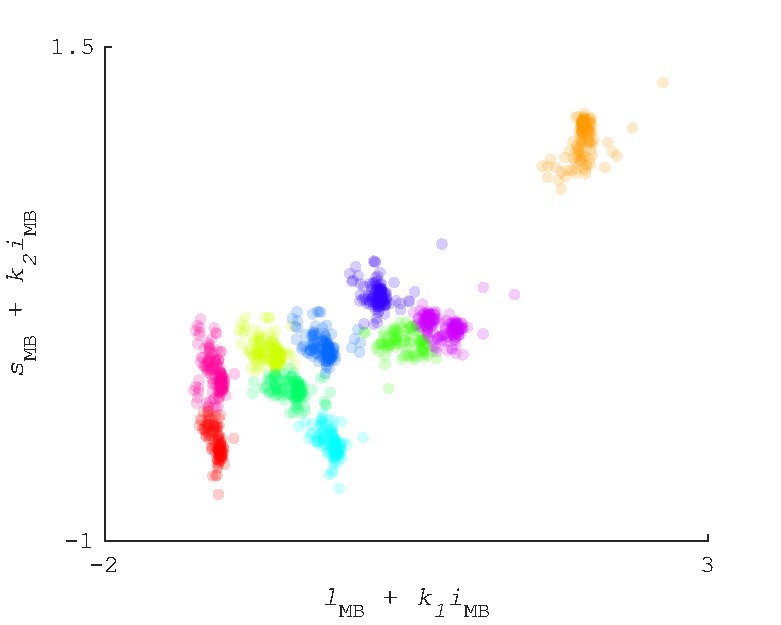
\includegraphics[max width=\textwidth]{figs/comp/KMeansMarkDemo/1.pdf}
 \caption{A reproduction of Figure \ref{fig:KM1} from Page \pageref{fig:KM1}, which shows the results of a k-means clustering of the data from Figure \ref{fig:corrected} from Page \pageref{fig:corrected} (which shows the \emph{actual} groups.}
 \label{fig:KM1lr}
\end{figure} 

The standard algorithm proceeds as follows: 

\begin{enumerate}
    \item $k$ random starting positions are assigned. 
    \item Each data-point is assigned a group based on which starting position is closest.
    \item The mean location of the data-points in each group is computed.
    \item Steps 2 and 3 are repeated, using the computed means instead of the original starting positions, until a stage where an iteration of these two steps results in no data-point changing groups. Once this occurs, the algorithm is said to have converged, and the resulting groupings are output.
\end{enumerate}

\subsection{Principal Component Analysis}

\textit{A valuable primer on \acrshort{PCA} in relation to colour technology is available from \citet{tzeng_review_2005}.}

\bigskip

\glsreset{PCA}
\Gls{PCA} is a dimensionality reduction method, used to to reduce the number of variables within a dataset whilst retaining as much of the variance as possible, and often used to identify the correlated roots of variance.

\begin{figure}[htbp]
 \includegraphics[max width=\textwidth]{figs/LitRev/PCA.png}
 \caption{Two-dimesional data with the first and second principal components added. Source: \url{https://commons.wikimedia.org/wiki/File:GaussianScatterPCA.svg}}
 \label{fig:PCA}
\end{figure} 

Along with similar techniques (such as single value decomposotion), it is used extensively within the study of daylight \glspl{SPD} \citep{hernandez-andres_color_2001,ojeda_influence_2012,pant_estimating_2009,bui_group_2004,judd_spectral_1964,maloney_computational_1984,spitschan_variation_2016} and natural \glspl{SRF} \citep{maloney_computational_1984,dzmura_color_1992,maloney_evaluation_1986,maloney_color_1986,cohen_dependency_1964,ferrero_principal_2011,zhang_reconstructing_2008,kwon_surface_2007,agahian_reconstruction_2008,harifi_recovery_2008,parkkinen_characteristic_1989,vrhel_color_1992,fairman_principal_2004,ayala_use_2006,eem_reconstruction_1994-2,connah_multispectral_2006,shi_using_2002,morovic_metamer-set-based_2006}. 

%A key goal for many of the researchers listed above... - how many dimensions/sensors do we need

In eras where the transmission of large datasets was troublesome, dimensionality reduction methods such as \gls{PCA} held value as a method to summarise a dataset, with the understanding that a reader could reconstruct a pseudo-dataset with minimal data-loss from the provided principal components. One such example is the work of \citet{judd_spectral_1964} where only the mean and first four characteristic vectors are provided\footnote{This is not technically \gls{PCA} but the related technique of \citet{morris_objective_1954}.}. The data from this study is replotted in Figure \ref{fig:Judd} and it can be seen that for their dataset this description does seem to offer a sensible summary of the data: the shape of the mean can be seen, and it can be seen that further variation principally occurs as a result of $V_{2}$ which is a broad and relatively monotonic function, indicating that changes are likely to be a skewing of the spectral shape.

\begin{figure}[htbp]
 \includegraphics[max width=\textwidth]{figs/LitRev/Judd.pdf}
 \caption{The mean and first four characteristic vectors of \citet{judd_spectral_1964}.}
 \label{fig:Judd}
\end{figure} 

\section{Interim Summary}

This chapter has laid out the most relevant developments in the research areas which the other chapters of this thesis build upon. 

Chapter \ref{chap:Interviews} builds upon our museum lighting knowledge by filling the gap in our understanding of how museum lighting is actually thought about and selected currently, and tries to identify the most fruitful avenue for future research which will allow the reduction of damage to objects in museums.

Chapters \ref{chap:LargeSphere} and \ref{chap:SmallSphere} target the interaction between colour constancy and \glspl{ipRGC}, using some of the methodologies covered in the Section \ref{sec:methodsforCC} and the knowledge of the physiology of \glspl{ipRGC} outlined in Section \ref{sec:ipRGCs} to build upon the experiments summarised in Section \ref{sec:ipRGCbeyond}.

Chapter \ref{chap:Tablet} investigates a new methodology (a variant of achromatic setting, described in Section \ref{sec:methodsforCC}) for performing colour constancy experiments, using museum spaces as test spaces due to their well controlled lighting environments.

Chapter \ref{chap:Melcomp} takes a more theoretical look at the relationship between colour constancy and \glspl{ipRGC} using a computational methodology, and the mathematical methods described in Section \ref{sec:math}.

\chapter{Research questions and hypotheses}

Are ipRGCs involved in colour constancy?

If they are, and we can undestand how they are, this may give us an insight into how to vary the \gls{CCT} of museum illumination in such a way that we can limit damage without degrading visitor experience.

%\chapter{Large Sphere Experiment} %new name?
\label{chap:LargeSphere}

\textit{The work presented here has been presented as an oral presentation at AIC 2013 \citep{macdonald_chromatic_2013} \textbf{prior to the author's involvement}, and as an oral presentation at ICVS 2017 \citep{garside_investigations_2017} by the author.}

Code and data is provided: \url{https://github.com/da5nsy/LargeSphere}

\section{Summary}

The goal of this experimental work was to examine the effect of different wavelengths of light upon chromatic adaptation. Our hypothesis was that \gls{ipRGC} stimulation may need to be considered in order to fully model the induced adaptation, with the null hypothesis being that chromatic adaptation can be fully accounted for by cone and rod mechanisms. If evidence of a melanopic input to chromatic adaptation were found, it may help to explain conflicting results in previous experiments which sought a `preferred \gls{CCT}', which may in turn allow for control of \gls{CCT} in museums to be used more extensively as a means to control damage to objects. 

This experiment is of a similar type to those discussed in Section \ref{sec:aadi}. Within a Ganzfeld viewing environment, illuminated by one of 16 different wavelengths of near-monochromatic light, observers performed an achromatic setting task, controlling the chromaticity of a display visible in the central field through a 4$^{\circ}$ circular aperture with two handheld sliders. Under these conditions it would be expected that an observer's chosen achromatic point would correspond in hue to the adapting field, and be of a saturation somewhere between a nominal objective white point and the adapting stimulus. If melanopsin were involved in chromatic adaptation we may expect unusual results for the part of the spectrum that melanopsin is most sensitive to (roughly 480nm).

Two different analyses were performed, with neither providing comprehensive support for rejecting the null hypothesis. However, it is noted that several assumptions are implicit in the experimental design, and that the experiment samples only a small region of the potential search space for melanopic input to adaptation (See Section \ref{sec:LSdis}).

This project was designed before the author arrived at \gls{UCL}, and data from two participants had already been collected. Data collection required at least 16 hours commitment from observers, and so the only observers up to that point had been LM (one of the author's academic supervisors), who initiated the experiment, and TR who was a student in the Medical Physics department. The original goal for my involvement in this project was that I should be a third observer, and assist in the data analysis. However, following the collection and initial data analysis of my own data, it appeared that there had been a technical fault during this run of data collection, and my data was deemed corrupted. Thus, my only contribution to this work is an extension to the data analysis started by LM, upon which I shall focus on in this chapter. The issue does not seem to have affected the data from the other two observers.

\section{Methodology}

\subsection{Hardware}

A hollow fibreglass sphere of approximately 750mm diameter was prepared with three holes; the first for an observer's face, the second (above the observer's head) for a light source to illuminate the Ganzfeld, and the third (opposite the first) through which a small portion of an LCD screen could be seen (A Fujitsu-Siemens SCALEOVIEW D19-1, SN:YE5L006100). A schematic is shown in Figure \ref{fig:sketch}.

\begin{figure}[htbp]
\includegraphics[max width=\textwidth]{figs/LargeSphere/sketch.png}
\caption{The hardware design. Illustration courtesy of Lindsay MacDonald.}
\label{fig:sketch}
\end{figure}

The screen was characterised such that calibrated stimuli could be generated. This was done by taking spectral measurements at 21 levels of pixel value for each channel, and later interpolating to create a full look-up-table to transform from pixel value to XYZ values and vice versa.

The interior of the sphere was painted with RAL 7040 dulux vinyl matt grey, of approximately 38\% reflectance. 

Illumination was provided by a Kodak slide projector with a tungsten-halogen light source, filtered through one of 16 near-monochromatic filters, ranging in 20nm intervals from 400-700nm inclusive. Measurements of the internal illumination were taken with a \gls{PR650} device, plotted in Figure \ref{fig:LSillum}. The illumination has been described further in \citet{macdonald_chromatic_2013}: ``The average luminance of the surrounding chromatic adapting field ranged from a maximum of 0.75 cd/m2 at 560 nm to less than 0.05 cd/m2 at the ends of the spectrum, corresponding to a retinal illuminance through a pupil of diameter 8mm ranging from 38 trolands (max) to less than 2.5 trolands, meaning that the viewing environment was in the upper mesopic range''. No effort was made to ensure that light from inside the sphere did not hit and/or reflect from the LCD display. 

\begin{figure}[htbp]
\includegraphics[max width=\textwidth]{figs/LargeSphere/LSillum.pdf}
\caption{The illuminations within the sphere, created by filtering light from a slide projector, measured as reflecting from a point just to the right of the aperture through which an observer would view the screen. Measurements made by Lindsay MacDonald.}
\label{fig:LSillum}
\end{figure}

\subsection{Observer task}

The observer sat on one side of the sphere with their face inside the sphere (as shown in Figure \ref{fig:Alejandro}), such that nothing outside of the sphere was visible. On view on the opposite side of the sphere was a circular 4$^{\circ}$ aperture onto an LCD screen, upon which a random colour was visible (See section \ref{sec:LSstim} for further details of the randomisation starting routine). It was the observer's task to use two handheld sliders, which controlled the chromaticity of the screen, to make the appearance of the screen achromatic (an achromatic setting task). On average it took observers roughly 20 seconds to make a selection. Once the observer was happy with the achromacy of the patch, a button was pressed to record the setting and a new random colour would be presented. The first displayed colour was at \gls{CIE} L* (of CIELAB and CIELUV) of 85, with subsequent colours descending by 5 L* until 10 L*. This sequence was repeated 10 times per session. Per session observers made 10 selections at 16 lightness levels (160 total). Observers performed 16 sessions (2560 selections total), one session for each adapting wavelength, visualised in Figure \ref{fig:ExperimentalPro}. Observers found sessions quite fatiguing and generally did not wish to do more than two or three sessions per day. A brief break was generally taken between sessions, though minimum time for such was prescribed.


In an additional (17th) session the narrow-band filter was replaced by a neutral density filter, to produce an achromatic adapting field.

\begin{figure}[htbp]
\includegraphics[max width=\textwidth]{figs/LargeSphere/Alejandro.jpg}
\caption{An observer sat at the sphere. Photograph courtesy of Lindsay MacDonald.}
\label{fig:Alejandro}
\end{figure}

\begin{figure}[htbp]
\includegraphics[max width=\textwidth]{figs/LargeSphere/ExperimentalPro.png}
\caption{The experimental protocol.}
\label{fig:ExperimentalPro}
\end{figure}

\subsection{Stimulus specification}
\label{sec:LSstim}

The stimulus was controlled via a MATLAB script, which read the input of two sliders and a button via a `Phidget' interface. The two linear sliders provided values of between 0 and 1000, and these values were converted to approximate CIELAB co-ordinates in such a manner that the slider maxima corresponded to the Natural Colour System (NCS) unique hue positions as computed by \citet{derefeldt_transformation_1986}. In this manner the sliders could be considered as moving along opponent axes between red and green (via the CIELAB origin), and blue and yellow (via the CIELAB origin) respectively. These values were transformed into standard XYZ values, with white references of [XYZ = 99.04, 100, 151.30] for observer LM and [XYZ = 94.97, 100, 98.15] for observer TR. It is unclear why these values were chosen, though it is suspected that at least one of them was the native white point for the display as measured at the time. These values were  then converted to display RGB signals using the GOG characterisation model and output to the screen.

The generation of random starting colours was achieved by modulating the nominal zero-point on each slider scale, where the default zero point is considered as 500, sampling from a uniform distribution between 250 and 750 for each presentation. 

The slider position was then considered relative to this new zero-point, meaning that once an observer hit the button to confirm their selection, a new random colour, anchored to their previous selection (in a rough manner) would be presented. It should be noted that this new colour was not entirely independent of the previous selection, due to this anchoring.

% \subsection{Data Collection}

% Data was collected for two observers \dots

\subsection{Data Processing}

Data were calibrated in the following manner: the recorded RGB values of the observers' selections were bounded (values above 1 or below 0, which occurred when observers made selections which were outside of the sRGB gamut, were brought within range, with an `absolute' rendering intent), quantized to 8-bits, and converted via look-up-table to \gls{CIE} 1931 XYZ tristimulus values. From these, xy chromaticities and CIELAB values were computed (with the white point of the display, as loaded from the characterisation file, used as the white reference).

A set of data referred to as the `baseline' data was generated, where there was no observer input, to consider the range of possible responses that an observer could make. This data was processed in exactly the same manner as the observer data, and is shown in Figure \ref{fig:overviewBL}, where it can be seen that the chromatic gamut increases as L* increases (due to a factor \texttt{cfac} in the display code which aimed to scale chromatic space with L*, mirroring the shape of CIELAB). It can also be seen that the gamut boundary is sometimes reached at higher levels of L*, with some of the vectors curving to remain within gamut.

\begin{figure}[htbp]
\includegraphics[max width=1.2\textwidth, center]{figs/LargeSphere/baselinedataOverview.pdf}
\caption{The baseline dataset. This data represents the condition where there is no observer input, and the two sliders are left at their maximum (1000), minimum (0), or neutral (500) positions (9 combinations). In the legend the first number denotes the slider A position, and the second denotes the slider B position.}
\label{fig:overviewBL}
\end{figure}

%The effect of the random offsetting was also queried, and it was found that the maximum random offset pushed the chromaticities halfway between \dots

Two distinct approaches were taken to data analysis. The first attempted to process the data in a chromatic space, with the reasoning that under the null condition chromatic selections should simply correspond to the chromaticity of the surround illuminations, presumably with some sort of gain function applied. If it could be shown that this relationship was not as expected, in a manner which might suggest involvement by other mechanisms (meaning rods or \glspl{ipRGC}), then this could be considered as evidence against the null hypothesis.

The second approach took advantage of the fact that measurements were taken at samples across the wavelength spectrum. Since we know the power at each waveband, and the spectral sensitivities of the receptors, we can see whether the responses (transformed to cone space) relate in some simple way to spectral sensitivities.

%Here the logic was that if the null condition were true, we should be able to fit a model to observer responses which only used cone-based inputs, and we could carefully consider the (presumed) benefit of including rods and \glspl{ipRGC} in the model. If either rod input or \gls{ipRGC} input were found to dramatically improve the model then this could be considered as evidence against the null hypothesis.

\section{Results}

\subsection{Summary}

Visually summarising the results for even a single observer is difficult due to the high number of variables and collected datapoints. In the following plots data is averaged over the 10 runs within each session (under each adapting wavelength). In Figures \ref{fig:overviewLM} - \ref{fig:overviewDG} data from LM, TR and the author (DG) is presented.

\begin{figure}[htbp]
\includegraphics[max width=1.2\textwidth, center]{figs/LargeSphere/LMdataOverview.pdf}
\caption{The dataset of observer LM. In all plots, the average CIELAB values are taken over the 10 repeats within each session. \emph{Top left:} an overview of the chromaticity of selected points. Connections between points indicate that they are from the same run (under the same adapting wavelength). Colouring of points and lines indicates the adapting wavelength, though whilst there is an approximate correspondence between the colour of the line and the appearance of the adapting field this is only meant as a means to differentiate between the different lines and is not in any way an accurate representation of appearance. \emph{Top right:} as for top left but only for points recorded at specific values of L*. Colours are as for top left, but lines linking points now represent points of like L*. This plot is included to show the relationship across wavelength of the adapting field. \emph{Lower left and right:} Other perspectives upon the CIELAB projection. Data as for top left.}
\label{fig:overviewLM}
\end{figure}

\begin{figure}[htbp]
\includegraphics[max width=1.2\textwidth, center]{figs/LargeSphere/TRdataOverview.pdf}
\caption{As per Figure \ref{fig:overviewLM}, but with the data of observer TR.}
\label{fig:overviewTR}
\end{figure}

\begin{figure}[htbp]
\includegraphics[max width=1.2\textwidth, center]{figs/LargeSphere/DGdataOverview.pdf}
\caption{As per Figure \ref{fig:overviewLM}, but with the data of observer DG.}
\label{fig:overviewDG}
\end{figure}

It can be seen in the data for all observers that there is a clear L*-dependent shift. Interestingly, the precise nature of this seems different for each observer; the data of LM clusters tightly around [0,0] for low values of L* and then generally moves north-west as L* increases, before returning towards the origin at the highest values of L*. For TR the shift is monotonic and roughly south-west.

Within this pattern it can be seen for observers LM and TR that there is a causal relationship between the adapting wavelength and the selected chromaticity. This is most easily seen in the top right plots of Figures \ref{fig:overviewLM} and \ref{fig:overviewTR}. In both cases a rough circle can be seen for both of the values of L* shown.

In Figure \ref{fig:overviewDG} it can be seen for observer DG in the lower-right plot that the data splits into two distinct groups, one of which is considerably lower in b* than is seen for either of the previous observers, or would generally be expected. It is suspected that there was a screen calibration issue which led to offsetting of the screen output in an unpredictable session-by-session fashion. It was found that a basic offsetting applied selectively to those sessions which appeared to be affected could `correct' for this issue, but without a better understanding of the issue this dataset is considered unsuitable for further analysis.

\subsection{Variability over time/repeats}

Not represented in the above plots is the way in which responses varied over time within each session, averaged over L* (the previous plots were averages over time). Figures \ref{fig:timeLM} and \ref{fig:timeTR} show the calibrated CIELAB values for observers LM and TR. 

L* should remain steady throughout (this was set), with minor differences introduced presumably due to differences between the screen and sRGB, 8-bit quantization, and any selections where a gamut boundary was reached. Both a* and b* follow the broad trends which would be expected given previous figures. Newly visible in these figures is the manner in which responses change over time. For both observers LM and TR the first two or three repeats seem to be distinct from the rest of the set, suggesting that adaptation had not yet reached a steady-state during this time.

\begin{figure}[htbp]
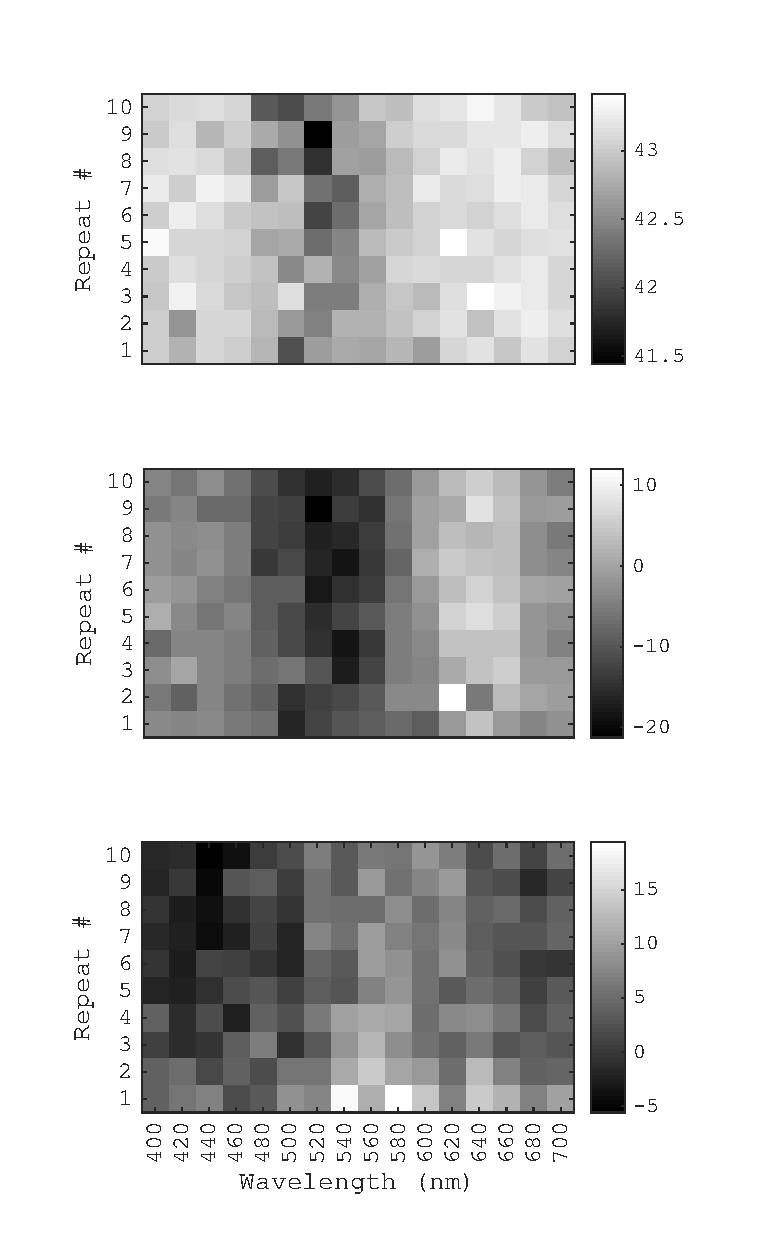
\includegraphics[max width=1.2\textwidth, center]{figs/LargeSphere/LMdataOverTime.pdf}
\caption{CIELAB co-ordinates across time (repeat number) for observer LM. Top plot is L*, middle a* and lower b*.}
\label{fig:timeLM}
\end{figure}

\begin{figure}[htbp]
\includegraphics[max width=1.2\textwidth, center]{figs/LargeSphere/TRdataOverTime.pdf}
\caption{As per Figure \ref{fig:timeLM}, but with the data of observer TR.}
\label{fig:timeTR}
\end{figure}


\clearpage


\subsection{Chromaticity-based analysis}

The CIELAB co-ordinates for the adapting fields were computed from the measurements shown in Figure \ref{fig:LSillum}, relative to the white point of the display for observer TR, and are presented in Figure \ref{fig:adapter1}. 

\begin{figure}[htbp]
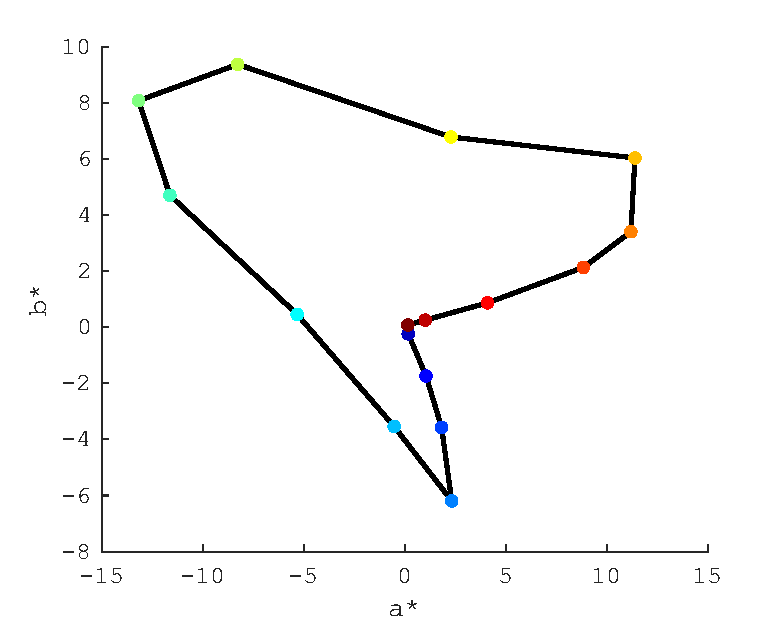
\includegraphics[max width=\textwidth]{figs/LargeSphere/adapter1.pdf}
\caption{The CIELAB values for the surround illuminations, calculated from the measurements shown in Figure \ref{fig:LSillum}, taking the white point of the screen (for the TR trials) as the white point.}
\label{fig:adapter1}
\end{figure}

If the surround fully controlled adaptation, and observers were fully adapted, it would be expected that observers would select the chromaticity of the surround as their neutral chromaticity. It is unlikely that either of these statements is correct, but we would still expect selections to be impacted by the chromaticity of the surrounds to some extent. If we re-plot the selected L* values from the top-right sub-figures of Figures \ref{fig:overviewLM} and \ref{fig:overviewTR} atop the data of Figure \ref{fig:adapter1}, we can visualise the correspondence between the observer selections and the surrounds\footnote{Note that the data of Figure \ref{fig:adapter1} is transformed for Figure \ref{fig:LMCompSurr}. The same measurements data was used for the surrounds, but the normalisation factor was different since the white point of the display was used when calculating CIELAB co-ordinates.}.

\begin{figure}[htbp]
\includegraphics[max width=\textwidth]{figs/LargeSphere/LMcompareWithSurround.pdf}
\caption{The CIELAB co-ordinates for the surround illuminations, relative to the white point used in the LM trials (black line), and the data from the top right sub-figure of Figure \ref{fig:overviewLM}, showing the CIELAB co-ordinates of the observer selections for 20 L* and 60 L* (dashed and dotted grey lines respectively).}
\label{fig:LMCompSurr}
\end{figure}

\begin{figure}[htbp]
\includegraphics[max width=\textwidth]{figs/LargeSphere/TRcompareWithSurround.pdf}
\caption{As per Figure \ref{fig:LMCompSurr} but for the data of TR.}
\label{fig:TRCompSurr}
\end{figure}

For both observers we see that the pattern of responses corresponds very well to the pattern of the chromaticities of the surrounds. For both observers there is a scaling and offset but considering the L* dependent shifts seen previously, and the way in which isoluminant planes through CIELAB change shape with changing values of L* this is to be expected.

Whilst there is some marked variation from a perfect replication of the surround CIELAB co-ordinates - for example the 500nm and 600nm points for LM, and the 520nm and 540nm points for TR, these variations seem to be in line with the level of noise in the responses, and attribution to a specific cause (such as melanopsin or rod input) cannot easily be achieved, since many variables are confounded.

Based on this analysis I do not find sufficient evidence to reject the null hypothesis.

% But luminance \dots

% \begin{figure}[htbp]
% \includegraphics[max width=\textwidth]{figs/LargeSphere/adapter2.pdf}
% \caption{As per Figure \ref{fig:adapter1}, but different perspectives upon the three-dimensional CIELAB space.}
% \label{fig:adapter2}
% \end{figure}

\subsection{Spectrum-based analysis}

%\textit{The code to reproduce the following analysis can be found at \url{https://github.com/da5nsy/LargeSphere/blob/master/Data\%20Analysis/VonKriesTest.m}}

The first stage of this analysis was to generate simulated data which represented the situation whereby there was only simple Von Kries adaptation. This was accomplished by multiplying the individual \glspl{SPD} (Figure \ref{fig:LSillum}) by the CIE 2006 10$^{\circ}$ observer fundamentals (not in the manner in which this is usually done, resulting in tristimulus values, but rather point-wise, thus retaining the spectral nature of the data). See Figure \ref{fig:LSsimdata}.

\begin{figure}[htbp]
\includegraphics[max width=\textwidth]{figs/LargeSphere/LSsimdata.pdf}
\caption{Simulated data for a basic Von Kries observer. In this figure white represents a high response. For example, with 560nm peripheral stimulation we would expect an observer to pick a colour with high L-cone activation as achromatic, assuming that the sensitivity of L-cones had been suppressed and thus higher activation was required to reach a neutral point (see peak roughly in the centre of the top bar).}
\label{fig:LSsimdata}
\end{figure}

A comparison was then made between this data and a set of real data (Obs = TR, averaged over time (entire run, no exclusions), averaged over L* = 35:60). This real data had been transformed from the recorded RGB values of achromatic matches into LMS values. It can be seen that there is a considerable difference between the simulated data and the real data (Figure \ref{fig:simVreal}). S-cone data shows the closest match, with the predicted peak at 460nm\footnote{Note that this is not at the peak sensitivity of s-cones (which would appear at 440nm for this dataset at 20nm intervals) but rather at the peak of the s-cone sensitivity function multiplied by the \gls{SPD}, as plotted in Figure \ref{fig:LSsimdata}.} being mirrored in the real data. This peak appears to bleed into the (real) M-cone data, and the simulated data for L and M-cone data shows very little correspondence to the collected data. Correlation coefficients between the simulated and this specific real dataset are 0.1399, -0.2509, 0.3164 for L, M and S respectively.

\begin{figure}[htbp]
\includegraphics[max width=\textwidth]{figs/LargeSphere/simVreal.pdf}
\caption{A comparison of simulated data (top row) and real data (bottom row). Data from the top row is as per the top three bars of Figure \ref{fig:LSsimdata}.}
\label{fig:simVreal}
\end{figure}

In order to understand the way in which adaptation may be crossing between channels, or the way in which we may have not properly isolated our channels (it is unclear exactly how much freedom an observer truly has to move around the response space) a brute-force method was used to find combinations of the above simulated data which would best fit the real data.

10000 random sets of weighting values (30000 values total) between -25 and 25\footnote{An analysis showed that the absolute range of these figures was unimportant, since we were looking for correlation with the real data rather than absolute correspondence. Thus they are listed here only to assist the reader in understanding graphs such as Figure \ref{fig:contributions_3}.} were generated. These weightings were applied to the simulated responses and the results were additively combined\footnote{(X amount of simulated L) + (Y amount of simulated M) + (Z amount of simulated S)}. The correlation between this new random combination and each channel of the real data was computed. The top performing randomly generated combinations were selected and are presented in Figure \ref{fig:maxsimVreal}. These particular combinations were created through cross-combining the original simulated data (top row of Figure \ref{fig:simVreal}), in the ratios shown in Table \ref{tab:crosscomb} and correlated with the real data to extent of the following coefficients: 0.9126, 0.8861, and 0.7726 for L, M and S respectively. These are much improved over the coefficients for the original simulated data.


\begin{table}[hbtp]
\centering
\begin{tabular}{|r|r|r|r|}
\hline
 & L & M & S \\ \hline
L & $18.4069$ & $-23.2578$ & $-10.9817$ \\ \hline
M & $-13.0477$ & $9.8327$ & $10.6844$ \\ \hline
S & $-2.7633$ & $-17.6798$ & $8.3036$ \\ \hline
\end{tabular} % Would be nice to format to fit page width
\caption{Optimal weights to fit the specific real dataset used. \\ \emph{Example: Image in top left of Figure \ref{fig:maxsimVreal} (L) was created by combining 18.4069 * the original simulated L (Top left of Figure \ref{fig:simVreal}), -23.2578 * the original simulated M and -10.9817 * the original simulated S.}}
\label{tab:crosscomb}
\end{table}

\begin{figure}[htbp]
\includegraphics[max width=\textwidth]{figs/LargeSphere/maxsimVreal.pdf}
\caption{A comparison of randomly generated combinations (top row) whereby channels were freely mixed from basic Von Kries simulated data (top row of Figure \ref{fig:simVreal}) to best correlate with real data, and real data (bottom row) (repeated from Figure \ref{fig:simVreal}).}
\label{fig:maxsimVreal}
\end{figure}

\begin{figure}[htbp]
\includegraphics[max width=\textwidth]{figs/LargeSphere/contributions_3.pdf}
\caption{Top 0.2\% performing randomly generated combinations, presented in terms of the weights of the original simulated data that they use. The subfigure on the left represents the weights needed to reconstruct the real data for L, the middle - M, and the right - S. Colour coded such that dark blue is the highest performing and yellow is the worst performing (of this highly performing subset).}
\label{fig:contributions_3}
\end{figure}

\begin{figure}[htbp]
\includegraphics[max width=\textwidth]{figs/LargeSphere/contributions_all.pdf}
\caption{As per Figure \ref{fig:contributions_3} but for all randomly generated combinations. The trends seen in Figure \ref{fig:contributions_3} are visible, and the range of these trends (extending into the poorer performing randomly generated combinations) can be seen. The colours are rescaled such that yellow now represents the worst performing randomly generated combinations of the entire set. Plots are plotted ordered by success and so lines representing successful randomly generated combinations will overlay lines representing poorer performing ones.}
\label{fig:contributions_all}
\end{figure}

The top performing 0.2\% of the randomly generated combinations are presented in terms of their components (analogous to plotting the values in \ref{tab:crosscomb}) in Figure \ref{fig:contributions_3}, and the entirety of the results for the randomised sampling presented in Figure \ref{fig:contributions_all}. 

It can be seen that to reconstruct the real data for L, a high amount of simulated L, and a low amount of both simulated M and S are required, though from Figure \ref{fig:contributions_all} it can be seen that the requirement for low S is less stringent. It can also be seen that the amount of L required seems related to the amount of M required (from the way in which the lines cross at a point).

A similar but opposite trend is visible for M.

For S, there is a narrow range of successful values for L (negative but close to 0), a larger range of strongly negative values for M, and a range of positive values for S. The reciprocal relationship between L and M seen in the reconstructions of L and M is no longer visible, but instead there is a new reciprocal relationship visible between M and S, though examination of Figure \ref{fig:contributions_all} suggests that this is not as important as in the case of L and M.

It is reassuring that in each case, successful random combinations used high positive levels of the target signal. For both L and S the target signal was the only positive weighting, with M taking positive weights of both M and S. 

\subsubsection{Adding rods and ipRGCs}

In order to investigate whether rods or \glspl{ipRGC} were playing a role in adaptation as measured by this dataset, the analysis was re-run with the additional rod input, additional \gls{ipRGC} input, and both rods and \glspl{ipRGC} as additional inputs. See Figure \ref{fig:LSsimdata} for a visualisation of these channels. The results of re-running the computations following the addition of these inputs is shown in Table \ref{tab:plusres}. Minor increases in correlation are exhibited. However, it should be noted that one would expect to see at least a minor increase in performance from practically any additional signal, so long as it was independent from the already accessible signals.

\begin{table}[hbtp]
\centering
\begin{tabular}{|r|r|r|r|}
\hline
Just cones: & $0.9126$ & $0.8861$ & $0.7726$ \\ \hline
+ rods: & $0.9156$ & $0.8881$ & $0.7987$ \\ \hline
+ ipRGCs: & $0.9218$ & $0.8867$ & $0.8055$ \\ \hline
+ rods + ipRGCs: & $0.9326$ & $0.8933$ &$0.8100$ \\ \hline
\end{tabular} % Would be nice to format to fit page width
\caption{Correlation coefficients for various conditions incorporating additional signals.}
\label{tab:plusres}
\end{table}

Further, it is not clear to what extent the gains exhibited in Table \ref{tab:plusres} are due to noise within the computations; the randomly generated combinations are set via a random number generator which is re-set each time the script is run for reproducibility, however there is nothing to stop the randomly generated values for the additional input runs performing better purely by chance alone. In order to investigate this, the above extensions were re-run 100 times each, and the top performance for each skimmed and saved. The results of this are presented in Figure \ref{fig:relcontributions}. From this figure it can be seen that there is a real and clear benefit from the inclusion of the additional signals, and from inclusion of \emph{both} of the additional signals.

\begin{figure}[htbp]
\includegraphics[max width=\textwidth]{figs/LargeSphere/relcontributions.pdf}
\caption{Raincloud plot \cite{allen_raincloud_2019} showing the results of re-running the extended analyses 100 times and skimming the best performer from each. Red points and probability density function represent `just cones', green - `+ rods', blue - `+ \glspl{ipRGC}', black - `+ rods + \glspl{ipRGC}'.}
\label{fig:relcontributions}
\end{figure}

\subsubsection{Spectrum-based Analysis Discussion}

There is a clear distinction between the simple simulated response functions, and the recorded data. It is interesting that a simple linear recombination can improve the correlation so greatly. It should be remembered however that this type of post-hoc fitting is liable to delivering whatever results a researcher might hope to find. 

Taken at face value, the results suggest that the principal drivers of adaptation are not at the cone level, but rather at a higher level, once cone inputs have been combined. The results mirror what might be expected of these higher level signals - there appears to be a single signal for L and M, roughly mirrored between the two, with a reciprocal trade-off possible between L and M for both, and the S cone signal takes positive weights for S, and negative weights for both L and M, but with a curious hint of a reciprocal trade-off between S and M.

However, it is unclear to what extent these relationships may arise due to limitations of the experimental set-up; it is possible that a rise in one signal is yoked through hardware limitation to the rise or fall in another. Future investigators should consider whether this effect is modellable.

Though there is a demonstrated ability of additional signals to improve the correlation with the real data, it would be a leap to consider this as evidence for the existence of mechanisms operating in this manner.

It is likely that any additional signal at a different wavelength (or even with a different frequency component) would have been able to deliver a higher correlation, since the data is noisy and through the random recombination we are functionally allowing every option to be tested. This is highly likely to result in over-fitting. One way to test whether this has occurred is to plot the contributions of the top performers from these situations (analogous to Figures \ref{fig:contributions_3} and \ref{fig:contributions_all}) and consider the apparent trends. This is plotted in Figure \ref{fig:contributions_5}. It can be seen that there do appear to be some trends for both rods and \glspl{ipRGC}. Splitting this apart, into Figures \ref{fig:contributions_4} and \ref{fig:contributions_5minusrods}, where we plot the results for simulations run where only the rods were added or only the \glspl{ipRGC} were added, we can see these trends slightly more clearly.

\begin{figure}[htbp]
\includegraphics[max width=0.9\textwidth]{figs/LargeSphere/contributions_5.pdf}
\caption{As per Figure \ref{fig:contributions_3} but for the conditions where both rods and ipRGCs were included as additional input signals were considered.} 
\label{fig:contributions_5}
\end{figure}

\begin{figure}[htbp]
\includegraphics[max width=0.9\textwidth]{figs/LargeSphere/contributions_4.pdf}
\caption{As per Figure \ref{fig:contributions_3} but for the conditions where rods alone were included as additional input signals.} 
\label{fig:contributions_4}
\end{figure}

\begin{figure}[htbp]
\includegraphics[max width=0.9\textwidth]{figs/LargeSphere/contributions_5minusrods.pdf}
\caption{As per Figure \ref{fig:contributions_3} but for the conditions where ipRGCs alone were included as additional input signals.} 
\label{fig:contributions_5minusrods}
\end{figure}

Figures \ref{fig:contributions_4} and \ref{fig:contributions_5minusrods} appear somewhat similar. Considering the similar spectral characteristics of rods and melanopsin, it should be expected that the model would use the signals in somewhat similar fashions. It appears as though neither has a particularly strong role to play in the L and M adaptation, however both seem to reliably be used as a negative weighting for S. It is unclear whether this is simply a response to a single high datapoint in this dataset (the peak at 460nm) or whether this integration serves a broader purpose. This peak at 460nm also seems to be the cause for the stubbornly low correlation coefficients for the S channel (compared to L and M), which max out at around 0.81 (see Figure \ref{fig:relcontributions}).

\section{Conclusion}
\label{sec:LSdis}

Two methods of analysis for the \citet{macdonald_chromatic_2013} data are presented here.

The chromaticity-based analysis showed that there was a strong correspondence between the patterns of the chromaticities of the adapting fields and the pattern of responses. There were a small number of outliers, which could plausibly be due to additional inputs to the adaptive process, however these outliers were in line with the amount of noise in the data, and confounded by many other variables and sources of noise. This analysis provides no basis for rejecting the null hypothesis.

The spectrum-based analysis showed that the results for one observer could not be well fitted by a simple model of Von-Kries-type observer, but that simple linear combinations of the responses of such an observer could be made to fit the recorded data very well. Though the ability of these fits is to be expected from this type of post-hoc fitting, the types of models which are predicted by the fitting align well with our understanding of post-receptoral signals, which suggests that we may be measuring adaptation at these levels. It would be particularly valuable to see whether the temporal nature of responses also aligned with our understanding of the timecourses of these different signals. It should be noted that this result could be due to the nature of the experimental set-up; observers were unable to modulate the cone activations directly. For example, to make the stimulus more green, the observer would inherently have to make it less red. It is plausible that this may account for the relationships seen in this analysis.

The second analysis further showed that integration of the simulated rod and melanopic signals provides additional value in fitting the data. Again, this is to be expected from this type of fitting. The minimal improvement delivered by the inclusion of rod and melanopic signals does not furnish me with strong enough evidence to reject the null hypothesis that chromatic adaptation can be fully accounted for by cone and rod mechanisms. 

\subsection{Limitations}

Several limitations have been identified with this experimental design which should be borne in mind when analysing this dataset, or planning similar experiments.

\begin{itemize}
\item The light levels in this experiment were in the mesopic range, and it is unclear whether we might expect to see melanopsin activation, and thus any melanopic interaction to adaptation, at these levels.
\item The light levels were different for each condition. Presumably a stronger adapting illumination might have a stronger adaptive effect, but it is unclear what how this might manifest (faster? more chromatic neutral point?) and what the underlying relationship may be. It would be tempting to match the adapting surrounds for luminance, or radiant power, but neither of these solutions provides genuine equality across conditions (when matching for luminance almost no level of 400nm radiation would be able to match the luminance at other wavelengths, and there is no reason why radiant power should directly translate to adaptive effect).
\item This experimental paradigm requires the assumption that adapting one part of the retina (the periphery) has an effect upon the adaptive state of another part (the fovea). This assumption is implicit in all chromatic adaptation models, but to some extent we know this to be incorrect - consider for example spatially locked after-images. See also the previous work of \citet{macadam_chromatic_1956} where two halves of the retina were explicitly adapted differently.
\item This method provides very noisy data, and it is difficult to average over any of the nominal `repeat' conditions since every variable seems to have a non-negligible effect, and none of these effects appear to be easily modellable. The inherent noise in this data collection methods places heavy limits on the scale of detectable effect sizes.
\item It is difficult to distinguish effects that indicate a biological basis and those which arise due to experimental limitations. For example, in the spectrum-based analysis it was unclear whether an increase in one sensor activation was required to make a match, or whether it was simply yoked to a decrease in another by the restraints placed upon the response space.
\item It appears that there is a strong correlation between an observer's match and the previous match. It is unclear whether this is due to the fact that the new `random' starting condition is centred upon the previous selection, or whether this is a foveal adaptive effect.
\item The spectral resolution of 20nm is relatively low for analyses such as the spectrum based analysis. However, increasing the resolution would probably be an unrealistic goal, considering the amount of required observer time.
\end{itemize}


\subsection{Further Work}

This dataset may only comprise data from two observers, but it is broad and may be valuable to those interested in chromatic adaptation and colour constancy. Various further analyses are envisioned:
\begin{itemize}
    \item As previously mentioned, there would likely be some value in the further modelling of the potential response space of an observer on this task, and the interaction the types of analysis performed here.
    \item It would be interesting to consider non-linear adaptation responses. This may better account for the data at the extremes of the wavelength range where luminance was very low.
    \item The temporal dimension of the data is not considered in either of the analyses presented here, but the code for the second analysis has been written in such a way that it should be relatively easy to implement. Considering the different expected time courses for adaptation for cones/rods/\glspl{ipRGC} this may serve to be a fruitful avenue.
    \item It would be valuable to collect data for more observers, ideally under conditions where the white point of the display was matched between observers, in order to understand what effects are robust across observers.
    \item If the L* dependent effects could be accounted for, then averaging over the entire range of L* could be implemented, which should reduce the level of noise, and improve the ability of an investigator to draw conclusions from a chromaticity-based analysis.
    \item For the spectrum-based analysis, currently only a single colorimetric observer is used (Stockman-Sharpe 10deg). It would be possible, and more correct to use specific observers relating to actual ages and visual fields. It may also be possible to use sharpened spectral sensitivities (see \citet{finlayson_spectral_1994}), though this would need to be done particularly carefully, considering the already large potential for overfitting.
\end{itemize}











%\chapter{Small Sphere}
\label{SmallSphereChapter}

Some stuff about things.\cite{example-citation} Some more things. 

Inline citation: \bibentry{example-citation}

% This just dumps some pseudolatin in so you can see some text in place.
\blindtext
\blindtext
\blindtext
\blindtext
\blindtext
\blindtext
\blindtext
\blindtext
\blindtext
%\chapter{The Tablet Method}
\label{chap:Tablet}

\textit{The work presented here has been presented previously as an oral presentation at AIC 2016 \citep[p. 125]{garside_estimating_2016}\footnote{Abstract available: \doi{10.6084/m9.figshare.4269680.v1}} and as a poster presentation at ECVP 2017 \citep[p. 93]{niko_busch_european_2017}\footnote{Poster available: \doi{10.6084/m9.figshare.5478493.v1}}}

\section{Summary}

The principal aim of this piece of work is to explore a novel method for colour constancy experiments, which allows for experiments to be performed in real and complex environments, in order to better understand colour constancy outside of a laboratory environment. The \gls{SAPS} method uses a tablet computer to present a spatial version of an achromatic point setting task. 

The key concerns are whether the proposed methodology can: a) present a stable stimulus across disparate environments, b) record differences in the state of chromatic adaptation, and c) be suitable for naive observers following minimal instruction. 

On each point, the method is shown to be moderately successful, with caveats, and suggestions are provided for improvements upon the current design. Such a methodology could be used to investigate the effect of multiple cues, conflicting cues and cues which cannot easily be reproduced in a laboratory environment.

Code and data are provided: \url{https://github.com/da5nsy/SAPS/}.

\newpage

\section{Introduction}

To further our understanding of colour constancy, investigators have traditionally designed well-controlled experiments where the number of variables is greatly reduced compared to a real-world environment. This allows investigators to carefully query the impact of any individual variable, or the interplay of a small number of variables. 

For example, a common stimulus-type used in such experiments are `Mondrian' patterns, arrangements of flat and unmoving overlapping coloured paper rectangles, see Figure \ref{fig:mondrian} \citep{hurlbert_colour_1999}. Consider also the experiments of \citet{kraft_mechanisms_1999} where objects representing potential colour constancy cues such as a tin-foil covered cone (specular highlights) were removed from a neutrally coloured box one-by-one in order to probe their relative usefulness as cues for colour constancy (see Figure \ref{fig:KraftBrainard}).

\begin{figure}[htbp]
\includegraphics[max width=\textwidth]{figs/tablet/mondrian.png}
\caption{An example `Mondrian', reproduced from \citet{land_recent_1986}.}
\label{fig:mondrian}
\end{figure}

\begin{figure}[htbp]
\includegraphics[max width=\textwidth]{figs/tablet/KraftBrainard.png}
\caption{A colour constancy experiment investigating the roles of different potential cues, reproduced from \citet{kraft_mechanisms_1999}. Objects within the scene were carefully selected such that the inclusion or removal or specific objects would allow or exclude the possibility of using a specific mechanism (local adaptation, spatial mean of the image, adaptation to the most intense region) to perform colour constancy.}
\label{fig:KraftBrainard}
\end{figure}

It is clear that these set-ups are much reduced in their complexity compared to a natural scene. Simple experimental stimuli allow for clear questions to be asked, and for those questions to be answered with statistical strength. Such research is valuable, but the results cannot always be extrapolated to other types of stimuli and different environments. The use of simplified stimuli risks overlooking unknown scene attributes, and the human behaviours which may be reliant on them. %LM: Ref Beau Lotto book
Experiments often find that colour constancy in lab environments is never `complete' \citep{murray_almost_2006,foster_color_2011}; is this representative of real world behaviour or could this result be due to a lab environment failing to deliver all the cues available to an observer in a natural environment? Recent technological advances have enabled experimenters to reproduce natural scenes with increasingly accuracy and comprehensiveness \citep{heasly_rendertoolbox3_2014}, but the number of variables in real scenes is practically infinite, and whilst our ability to reproduce a scene increases over time as technology develops, we only reproduce what we deem important at the time. Using a real-world environment would allow for processes to occur as they do naturally, in the environment for which these processes are presumably optimised (See \citet{kelly_chips_2018} and \citet{shepard_perceptual_1992}). The ability to move away from the lab environment also allows us to run experiments in specific locations of interest, such as museum spaces.

There are at least two clear challenges to the use of natural environments for scientific study; the inability to control target variables, and the influence of uncontrollable or uncontrolled non-target variables. The first challenge may be surmountable; depending on the variable in question it might either be controlled by force, or over time natural variability may provide the required experimental range. The second may be insurmountable but, depending on the specific situation, it may be permissible to consider uncontrolled variations simply as sources of experimental noise. Further challenges arise where connections exist between target and non-target variables, or where the influence of the non-target variables dwarf the effect of the target variable.

One further challenge: it is rare for an experiment in a real-world environment to not intrude onto that real-world scene and change it in some way. The only true solution to this problem would be to consider unannounced observation of a natural behaviour as the only acceptable scientific method, which would be incredibly restrictive and impractical. A pragmatic compromise is to design an experiment such that it modifies the environment of the observer minimally, and to consider carefully the impact that the experimental set-up may have upon observers. This is the approach which shall be taken here.

The method presented here is a variant of the `achromatic setting' method.\footnote{For an overview see Section \ref{sec:methvis}, or
the section on `achromatic adjustment' in \citet{foster_color_2011} and `Matching to an internal standard' or `achromatic setting' in \citet{smithson_sensory_2005}.} The achromatic setting method requires an observer, under specific conditions, to adjust the chromaticity of an item in their visual field such that this item appears achromatic. Changes in selected achromatic point (in colour space) are thought to represent general adaptive shifts. For example, an observer in an environment lit by a chromatic illuminant would be expected to pick an achromatic point which is shifted towards the chromaticity of the illuminant, compared to the achromatic point which they might select in a more neutral environment. This is often practically achieved by having the `object' be an area of a computer screen, and have it controllable in two or more chromatic dimensions (such as relative amounts of unique red/green and blue/yellow). 
%LM: refernces

In the \gls{SAPS} method, as presented here, a tablet computer is given to an observer to hold as is comfortable to them, and upon this computer an isoluminant slice through a nominally perceptually uniform colour space is presented, from which they are requested to select (by touching upon the screen with a finger) the point which they deem to be most achromatic (the specific phrase `grey-est or least colourful' is employed in order to make the task suitable for non-colour-scientist observers). The term `spatial' is used since the user provides information by making a spatial selection which directly corresponds to a colour choice, where in other methods abstract sliders or knobs may be used to alter the chromaticity of a static object.

To minimise the effect of the presentation of chromatic scenes upon the viewer, which may influence an observer's state of chromatic adaptation, this process is repeated a number of times with the area of colour space which is presented varying, through random rotation about the luminance axis, and random offsetting through both dimensions of the chromatic plane.

The rest of this chapter shall describe the method in more detail, and some experiments performed to explore the potential abilities and limitations of this method.

\section{Research Questions and Hypotheses} \label{sec:qandhyp}

\subsection*{Hypothesis 1: The \gls{SAPS} method is suitable for colour constancy experiments}

To be fit for performing colour constancy experiments, this method needs to:

\begin{enumerate}[label=\Alph*.]
    \item \label{list:hyp1a} \emph{Provide a relatively environment-agnostic stimulus.} 
    This experimental method relies on the assumption that the tablet display delivers a stimulus with identical physical properties to the observer independent of environment, with no effect of ambient illumination. In practical terms, this means that the tablet must not be affected by reflection, either at the glossy surface of the tablet display, or at reflection at any other level of the display architecture, to the extent that this has a non-negligible impact upon recorded data. If it is found that this is not the case, the tablet would need to be characterised separately for each environment.
    \item \label{list:hyp1b} \emph{Collect meaningful data.} 
    One would expect this to be indicated by small intra-observer variability (not recording a change where there is presumably none), and reasonable inter-environment change (recording a change where there is presumably a change). It would be expected that these changes would be in line with previously published results. An implicit assumption is that an observer's achromatic point will align with the chromaticity of the ambient illuminant.
    \item \label{list:hyp1c} \emph{Additional aim - Be suitable for naive\footnote{In this instance by `naive' I mean non-colour-scientist (a large number of colour vision experiments have been run only with colour scientists as observers and it is possible that this has biased results) and untrained (it is relatively common for this type of experiment to require extensive training upon a colour naming system such as The Munsell System of colour, by which participants are asked to report the appearance of a test object.)} observers.}
    This would reduce the amount of time and effort required to run experiments, and allow for the collection of data from participants less likely to be biased through task expectation. It also means that the demographic group of observers is less likely to be 
    WEIRD (`Western, Educated, Industrialized, Rich, and Democratic', \citep{henrich_weirdest_2010,brookshire_social_2013,justsaysinweird_just_2019}), white, and undergraduate.
\end{enumerate}

\subsection*{Hypothesis 2: \gls{ipRGC} activation affects perceptual white point.}
Primarily as a proof of concept for this methodology, but also to assist in answering other research questions posed within this thesis, an experiment was performed whereby observers made achromatic selections under a selection of colorimetrically metameric illuminants where there was a melanopic contrast between illuminants.
If \glspl{ipRGC} play a role in colour constancy we would expect to see a distinction between the responses recorded under the different illuminants. If the results of \citet{cao_evidence_2018} were to be reproduced, we would expect to see a distinction along $l$ pathway isolating directions and not along $s$ pathway isolating.

\section{Experimental set-up and methodology}

Three separate experiments were performed. These are described in Section \ref{sec:SAPS_exp}.

\subsection{Participants}

\subsubsection{Selection of participants}

The participants for Experiment 1 (Section \ref{sec:SAPS_exp1}) were the author, one of the author's academic supervisors (KC) and a technician at the laboratory (TS).

For Experiment 2 (Section \ref{sec:SAPS_exp2}), 58 observers were selected randomly from museum visitors. A visitor would be approached by the experimenter (the author) and asked whether `they would be interested in taking part in a colour vision experiment'. Those who replied positively were verbally informed of the ethics details for the study, the principal parts of which were: that no identifying information would be recorded, that the experiment carried no risks greater than those associated with normal use of a tablet computer, that observers were not paid or otherwise incentivised to take part, and that the task would take roughly ten minutes. A verbal description of the ethics details for this experiment was provided rather than the more traditional paper version to avoid providing the observer with a white reference immediately prior to the experiment. This study was approved by the \gls{UCL} Ethics committee (Project ID Number: 9357/001), application attached as Appendix \ref{app:ethics1}. In accordance with the ethics approval granted for this project, people under the age of 18 were only invited to participate under the supervision of a parent/carer.
% number, age and sex here? !!!!!!!!!

For Experiment 3 (Section \ref{sec:SAPS_exp3}), nine participants (5 female, 4 male, ages not recorded) were recruited from the author's friends and family (including one academic supervisor, LM), with the hope that this would assure attendance and motivation and to take advantage of short-notice availability of the experimental space. Participants were informed of the ethics details for the study in advance of attending. Ethics approval was provided following the amendment of the aforementioned ethics application (9357/001), attached as Appendix \ref{app:ethics2}.
% number, age and sex here? !!!!!!!!!

\subsubsection{Instructions to the participants}

The observer was instructed to hold the tablet such as was comfortable for them to do so, upon which the first trial of the experiment was already visible (see Figure \ref{fig:grant_demo}). They were instructed to `touch the grey-est, or least colourful, point on the screen'. Upon touching the screen, the stimulus would be replaced with a new stimulus. This new stimulus was a new subsection of the full stimulus image (See Figures \ref{fig:finger} and \ref{fig:Stimulus}) which had been randomly rotated and offset (further information provided in Section \ref{sec:stimuli}).

\begin{figure}[hbtp]
\includegraphics[max width=\textwidth]{figs/tablet/MVI_3213-1.jpg} % E:\Pictures\2016\2016-10-14
\caption{A participant (the author) holding the tablet with a stimulus on screen.}
\label{fig:grant_demo}
\end{figure}

\begin{figure}[hbtp]
\includegraphics[max width=\textwidth]{figs/tablet/MVI_3889-4.jpg} % E:\Pictures\2016\2016-10-18
\caption{A stimulus displayed upon tablet and finger in motion towards subjective point of achromacy.}
\label{fig:finger}
\end{figure}

Most observers seemed to find this task difficult for the first stimulus (appearing confused and often verbally expressing difficulty), but within the first few stimuli seemed to develop an increased comfort and ease with the task, resulting in a decreased response time (Figure \ref{fig:mediantime}). At this point the observer was told that there would be thirty trials. No observers dropped out mid-session. No training was provided, and no runs were excluded as training runs. One stimulus was forced to have identical rotation and offset to an earlier stimulus, in order to assess intra-observer variation (see Section \ref{sec:exclusion}).

Following the thirty trials, a secondary task was presented to observers, designed to characterise their touch input. This task features a 2x2 checker board pattern upon a black background (See Figure \ref{fig:checker-board}). Observers were instructed to touch the centre of this checker board. Upon registering a touch, a new checker-board would be presented, of the same attributes but modulated in position in the same way as the main stimulus. This stimulus is presented 10 times. This data was later used to calibrate touch input, and to ascertain the amount of measurement uncertainty derived from touch input. %!!!!!! This is doing weird formatting, check before submission

\begin{figure}[hbtp]
\includegraphics[max width=\textwidth]{figs/tablet/checker_board.png} % E:\Pictures\2016\2016-10-18
\caption{Photo of checker-board task. Participant is requested to touch centre of the checker-board pattern.}
\label{fig:checker-board}
\end{figure}

% \clearpage %currently ending up with a single line which looks dodgy, check later %!!!!!!!!!!!!!

%Doing this without incentive for participants meant that it was rushed (?)

\subsection{Stimuli} \label{sec:stimuli}

\subsubsection{Selection of stimuli colour space}

The stimulus presented to observers was an isoluminant plane (in CIE L*) through CIELUV colour space. CIELUV was chosen, over CIELAB or CIECAM02 for example, since it has an associated object colour space (\gls{CIE} u'v', see Section \ref{sec:speccolspac}), which allows for comparisons between the chromaticity of light sources and the chromaticity of selections to be made\footnote{Some preliminary runs of the experiment, performed at The UCL Grant Museum, used a stimulus defined in CIELAB colour-space instead, before later changing to CIELUV for the reason above.}. 

\subsubsection{Generating the stimuli}

The stimulus was specified as: L*: 60 uniformly across field, u*: ranging linearly from -50 to 50 from one side of the field to the other, and v*: as for u*, but along the orthogonal axis, so that the stimulus was of uniform lightness and smoothly changing hue and chroma. The full stimulus image (Figure \ref{fig:Stimulus}) was 2188 x 2188 pixels; this is larger than the pixel dimensions of the chosen screen (1366 x 768, Section \ref{sec:spec}) to allow for the stimulus to be rotated freely and offset by up to a third of the image in any direction before the edge of the image is encountered. 

The stimulus was specified with the above attributes in a matrix within \gls{MATLAB}\footnote{Code: \url{https://github.com/da5nsy/SAPS/blob/21940bb6ed9d0e37d88e1b655f4919d73431743a/experiment/stimulusGenerator002.m}}. CIELUV values were converted to XYZ tristimulus values, with reference white set as the XYZ tristimulus values of the display at maximum white (with screen protector), as measured with an Xrite i1 device (shown in Figure \ref{fig:gamut}). Linearisation was achieved through the use of a look-up table, computed by spline interpolation of the measured outputs at 15 pixel %(KT: pixel drive value?)
value increments from 0 to 255 for each channel. The stimulus was then output as an 24-bit RGB tiff, which could be easily loaded and manipulated by the psychophysical stimulus presentation software PsychoPy \citep{peirce_psychopypsychophysics_2007}. %(Illustrate with flow diagram?)

\begin{figure}[hbtp]
\includegraphics[max width=\textwidth]{figs/tablet/stimulus.png}
\caption{Full stimulus image, from which subsections were selected and presented as stimuli. Note that no effort has been made to correct this image for printing, and so it is best considered as only a rough approximation. It may be possible to see the vertical line on the left where the sRGB gamut boundary is reached; this is further described in Figure \ref{fig:stimchan}.}
\label{fig:Stimulus}
\end{figure}
% Copied and pasted from original psychopy folder. Could regenerate using stimulusGenerator002.m

\subsubsection{Presenting the stimuli} \label{sec:presenting_the_stimuli}
A program was written in PsychoPy\footnote{\url{Code:  https://github.com/da5nsy/SAPS/blob/21940bb6ed9d0e37d88e1b655f4919d73431743a/experiment/SpatialAchromaticPointSetting_0940_Grant.py}} that presents the stimulus 30 times%LM: need discussion of why 30 times
, with random rotation and random offset in the horizontal and vertical dimensions of between -1/6 and +1/6 of the respective dimension. Thus the `objective white point', where [u*,v*] = (0,0), was always within the central third (in each dimension) of the screen. This program saved details of the stimulus offset and rotation (`dpX', `dpY' and `ori'), co-ordinates of observer selected point (`x-co\_raw', `y-co\_raw', and also `direction\_raw', `magnitude\_raw'), and time taken to make selection, measured since last selection (`toc\_raw').

The effect of rotation and offset was such that on each stimulus presentation the observer saw a stimulus that appeared somewhat different to the previous stimulus, but still hopefully included their perceptual achromatic point. %The rotation and offset can be illustrated by plotting the chromaticities present in any one stimulus presentation, as in figure X. %!!!!!!!!!!!!!!!!!!!
Plotting the chromaticities present across a full run of 30 trials yields Figure \ref{fig:practical}, where it can be seen that the rotation results in a roughly circular spread of chromaticities, and the rotation and the offsetting together result in a gradient of likelihood of presentation which is high at the centre of the full stimulus and lowest at the edges of the full stimulus. This gamut distribution is referred to further in the text as the `practical gamut'.

% Single shot figure needed

% \begin{figure}[hbtp]
% \includegraphics[max width=\textwidth]{figs/tablet/????}
% \caption{A representation of the chromaticities present in a single stimulus. Note that the gamut is not rectangular for 2 reasons: firstly, because CIELUV is not a linear transformation of CIE u'v' , and secondly because for this particular stimulus, the bottom left corner (as presented above) intersects with the display gamut boundary, resulting in a gamut compression to that corner.}
% \label{fig:?????}
% \end{figure}


\begin{figure}[hbtp]
\includegraphics[max width=\textwidth]{figs/tablet/practical_gamut.pdf}
\caption{The `practical gamut' (shown in colours ranging from dark blue to yellow), within the device gamut (dashed lines). This plot shows the relative frequency that chromaticities are actually presented, within the device gamut (more fully described in Figure \ref{fig:gamut}). The highest number of times a particular chromaticity can be presented is 30, since there are 30 trials in a typical run. Chromaticities falling towards the objective white point of the stimulus (where [u*,v*] = (0,0)) are presented every stimulus, whereas those further away from the centre of the stimulus are presented less frequently. On the left-hand side of the cluster it can be seen that the gamut boundary is reached.}
\label{fig:practical}
\end{figure}

\subsubsection{Limitations of the stimuli} \label{sec:limitations}
Under the current set-up the stimulus is to some extent fixed; each stimulus is a subsection of a single complete stimulus image (Figure \ref{fig:Stimulus}). This means that an observer can at no point select a chromaticity that is not present in the full stimulus, and they will less often have the option to select a chromaticity which falls towards the boundary of this stimulus space than they would be able to select one at the centre of this space, due to the nature of the rotation and offset described in Section \ref{sec:presenting_the_stimuli} (See Figure \ref{fig:practical}). 

When designing the stimulus it was assumed that the stimulus would cover a large enough area of colour-space to allow for any selection that an observer would reasonably care to make (the stimulus would include an achromatic area surrounded by areas which under no situation would be deemed achromatic). Later analysis (for example, see Figure \ref{fig:PAMELA_DG_results} where an illuminant falls far outside the practical gamut) showed that this was not the case, and that it was not unusual for an illuminant that appeared entirely neutral to fall outside of the response-space. I had underestimated the power of colour constancy!

This limitation leads to a pattern in the data which I shall refer to as `smearing', so called because when the desired selection point is outside of the practical gamut, or even close to the edge of the gamut, the closest possible points which are available for an observer to select will fall upon a line between the objective white point (where [u*,v*] = (0,0)) and the true desired selection point, thus the data is smeared between the point which an observer actually wants to select, and the objective white point. This is discussed further is Section \ref{sec:bounding}, where amendments to this experimental method are proposed which might limit or remove this effect.

A visual example of this can be given by considering the results of an amended experiment where the same stimulus was presented but the question changed to `touch the X-est point on the screen' where X was red, green, blue or yellow. See Figure \ref{fig:basement_rgby_test}, where the responses for chromatic questions have a much larger spread than that for the achromatic question (in grey, centre) and tend to show characteristic orientations of spread - from the outer regions of the practical gamut towards the centre. This is a more extreme case than a white-appearing light source outside of the practical gamut but it is thought that the effect upon the data would be similar.

\begin{figure}[hbtp]
\includegraphics[max width=\textwidth]{figs/tablet/basement_rgby_test.pdf}
\caption{Results from an amended experimental paradigm to demonstrate `smearing'. The observer was asked to `touch the X-est point on the screen' where X was red, green, blue or yellow. Background dots are sub-sampled from the practical gamut, to indicate ability of the observer to select specific chromaticities, as shown in Figure \ref{fig:practical}. A normal run of the experiment was conducted under the same conditions at the same time to provide a baseline condition.\\ 
The experiment was performed in the basement of the Chadwick Building (Section \ref{sec:Chadwick}) with the author as observer.}
\label{fig:basement_rgby_test}
\end{figure}

A broader limitation, which applies to all screen-based experiments, is that regardless of the gamut of the stimulus used (here `practical gamut') we are operating within a larger fixed gamut, shown within Figures \ref{fig:practical} an \ref{fig:gamut}. It can be seen in Figure \ref{fig:practical} that our chosen stimulus gently nudges the left-hand gamut boundary of the screen. This can be thought of as a request for colours which are less red than is possible using this specific display.

The effect of this could be reduced by choosing a screen with a particularly large gamut. A drastic alternative might be to consider a reflective screen device (such as a Kindle or other e-reader/e-ink device) but this would immediately fail Hypothesis 1A (\emph{`Provide a relatively environment-agnostic stimulus'}) and so the device would need to be characterised within each new environment, which reduces the appeal of this method considerably.

Another limitation with this type of stimulus/set-up is that if observers were to treat the screen as an emissive device they might treat the colours displayed as unrelated to the environment, and thus simply select a moving average of the colours which had been displayed on the screen, which would eventually (over enough trials) average to be the nominal white point (centre) of the stimulus. This is discussed further in Section \ref{sec:LargeVisualAngle}. 

\subsubsection{Touch input characterisation} \label{sec:touch}
The checker-board stimuli (Figure \ref{fig:checker-board}), included to allow for fine spatial calibration for individual observers' touch input, was generated by running the main experimental script again but with the stimulus file path replaced with a simple pattern generated within PsychoPy.

I hypothesise that any shifts in touch input would be the result of one or both of two potential influences: personal finger offset and general hardware calibration. By the former I refer to the fact that whilst a finger is considered to be a relatively discrete unit, controlled with presumed dexterity and accuracy, the specific part of the finger which touches the screen will vary from person to person, with each person exhibiting a reliable bias. By the latter I refer to the fact that it is highly possible for there to be a `fairground gun effect', whereby the hardware introduces a reliable bias due to calibration misalignment, which affects every observer equally.

Performing a calibration of each observer's data based on this individual characterisation allows for offsetting of both of these types of variation. 

\subsection{Specification of Tablet PC} \label{sec:spec}

Participants undertook the experiment upon a Dell Latitude 10 ST2 tablet computer (223x126mm active screen area, 1366x768 pixels) with `BROTECT' Matte Screen Protector (a thin adhesive, translucent, and matte screen protector). This tablet was chosen for its ability to run a Windows environment, and the screen protector was added to reduce the severity of specular reflections. The measured gamut of this device is shown in Figure \ref{fig:gamut}, with the gamut of sRGB for comparison.

\begin{figure}[hbtp]
\includegraphics[max width=\textwidth]{figs/tablet/gamut.pdf}
\caption{The display gamut, plotted in CIE u'v' space. Red, green and blue dots indicate chromaticities of single channels at pixel values from 0 (central values) to 255 for each respective channel. The black dots are the chromaticities achieved when the pixel values are kept in line for each channel. This can be described as the native white point of the display, and can be seen to drift leftwards and then downwards as pixel values increase.}
\label{fig:gamut}
\end{figure}
% Generated using the 'Plot gamut' section of SAPS_TabletCharacterisation.m

\subsubsection{Impact of ambient illumination} \label{sec:ambient}

A key requirement in this methodology is that the display device remains roughly colorimetrically stable across a range of lighting environments (see \hyperref[list:hyp1a]{Hypothesis 1A}). This would only be true if the device produced the entirety of the light emanating from it in normal use. In reality, a small amount of light will be reflected from the surrounding environment. This may be reflected either at the surface layer of the screen (specular reflections) or at a lower level of the screen architecture. Here we aim to quantify the amount of light reflected in this way, understand the impact that this has on this method, and seek to minimise this impact if possible.

It is assumed that specular reflections are clearly distinguishable to most users, and that users will automatically hold the device in such a way as to minimise their interference with the task. It is also assumed that the spatial nature of such reflections and the fact that they are not locked to the geometry of the screen (but rather move as the screen or observer moves) would further allow an observer to visually discount them and not confuse them for an output of the screen.

The key concern then is reflection at other levels of the screen architecture. Using the screen calibration framework \cite{berns_crt_1993}, this may be considered as an environment-dependent `offset', that is, a figure which is added to the output of the screen at all levels. It is assumed that this level is constant in an unchanging environment, and independent of the output of the screen. It therefore follows that this will have greatest impact on the chromaticity of the display at low luminances, where the amount of reflected light is high relative to the output of the display.

To consider whether such reflections exist for our specific set-up, telespectroradiometric measurements were taken of screen at varying pixel value levels (0 to 255, intervals of 15)\footnote{Code: \url{https://github.com/da5nsy/SAPS/blob/master/auxiliary_functions/tablet\%20characterization/calibration.py}} under 3 different lighting conditions (Warm White (`WW') : [u'v'] = [0.248,0.524]; Cool White (`CW') : [u'v'] = [0.200,0.465)], Mel-High (`MH') :	[u'v'] = [0.201,0.467], further described in Section \ref{sec:PAMELA}) One condition was repeated to assess measurement uncertainty. The measurement device used was a \gls{PR650}. The set-up is shown in Figures \ref{fig:pr6501} and \ref{fig:pr6502}.

Broadly speaking, at a pixel value of 0 one would expect that the illumination reaching the position of the observer depends almost entirely upon the illumination (entirely, if we assume that the black of the screen is uniformly spectrally reflective), whereas at maximum output (pixel values of 255 in all channels) the illumination reaching the position of the observer would be greatly more dependent upon the output of the device, hopefully with negligible influence of the illumination (so long as the illumination was below a certain threshold). The point of interest is therefore assumed to be the pixel value where the shift resulting from differing illuminants jumps from being non-negligible to negligible for our purposes.

\begin{figure}[hbtp]
\includegraphics[max width=\textwidth]{figs/tablet/pamela_pr6501.jpg}
\caption{The measurement set-up at \gls{PAMELA}. PR 650 on right, with control PC on left, and tablet in the centre.}
\label{fig:pr6501}
\end{figure}

\begin{figure}[hbtp]
\includegraphics[max width=\textwidth]{figs/tablet/pamela_pr6502.jpg}
\caption{The measurement set-up at \gls{PAMELA}. The tablet computer, showing the characterisation routine (on the left of the screen). Note the specular highlight on the left of the tablet frame, reflecting the detail of one of the many \gls{LED} arrays overhead.}
\label{fig:pr6502}
\end{figure}

As shown in Figure \ref{fig:pr6503} it was found that for pixel values of 60 and below there was a considerable chromaticity variation between data from each lighting condition. This aligns with our expectation that the greatest effect would be seen at lower screen output levels.

\begin{figure}[hbtp]
\includegraphics[max width=\textwidth]{figs/tablet/pamela_pr6503.png}
\caption{Chromaticity co-ordinates of measurements at different pixel values, under 3 conditions (Warm White (`WW') : [u'v'] = [0.248,0.524]; Cool White (`CW') : [u'v'] = [0.200,0.465)], Mel-High (`MH') :	[u'v'] = [0.201,0.467], further described in Section \ref{sec:PAMELA}). `WW2' is a repeat of the `WW' condition. It can be seen that the 0 values (where the screen is effectively off) diverge greatly. They do not diverge in exactly the directions of the chromaticities of the light sources, which could either be due to measurement inaccuracy, or the base colour of the tablet may not be perfectly spectrally neutral. At higher pixel values the chromaticities start to converge at around [u',v'] = [0.193,0.47].} %would be nice to reproduce, current figure is rendered weirdly !!!!!!!!!!
\label{fig:pr6503}
\end{figure}

%LM: plot measured luminance vs pixel value

For values above 75 (inclusive), a conservative estimate for the maximum shifts in chromaticity due to variation between light sources (considering only those sources tested) would be roughly 0.004 in the u' axis, and 0.009 in the v' axis. These values are derived from visual inspection of the variation in values of chromaticity for readings taken of pixel values above 75. These figures could be considered baseline figures for classifying observed differences as likely to originate from genuine changes in observer state rather than lighting/stimulus artefacts.

It is noted that the variation between the repeated measurements, denoted `WW' and `WW2', is larger than might be expected; at high pixel values the chromaticities recorded under `CW', `MH' and `WW2' converge very well, but `WW' seems offset by roughly 0.005 units in a roughly north-east direction in colour space. The cause of this is unclear. The cause could be the result of `warm up' (either in terms of an actual temperature dependency, or in terms of a device taking time to settle into a default operating mode after turn on) of either the screen or the spectroradiometer. It could also be the case that between measurements the angle of the screen relative to the spectroradiometer changed and that this was the cause of the distinction. For this type of display it is well known that there are generally significant effects of angle of view. No attempt was made to force participants to hold the tablet at a specific angle, assuming that observers would naturally hold the tablet in a manner which would place it perpendicularly to the line of view. Any attempt to force a specific viewing angle would have limited the accessibility of this methodology. 

% ----------% This is all well and good but not required. 
% Consulting the spectral data for `WW' and `WW2' (Figure X%!!!!!!!!!!!
% ) we can see a systematic variation whereby for the initial `WW' run the recorded values for lower wavelengths are slightly lower, and the higher wavelengths record slightly higher values, when compared to the `WW2' data.

% % figure

% Another way of representing the above is to consider the effect that changing lighting has on the recorded spectral power distribution of light entering an aperture at the rough location of an observer's eye.

% % figure
% % [Caption: The recorded spectral power distributions, for each measured level of pixel value, under each of the 4 illuminations. Plots are limited to lower pixel values for attention.] Need to find a better way to present this

% Above, it can be seen that at lower levels of pixel value, the spectral power distributions are notably different between lighting conditions. Under `MH', for example, there is a noticeable difference in \gls{SPD} shape whereby at the lowest pixel values there is a peak around 470nm, which quickly fades from notice as pixel values increase. For `CW' in comparison, we can see that the 450nm peak is substantially higher at low pixel values than at either of the `WW' measurements, suggesting that this light source provides additional power at these wavelengths.

% In all the cases above, the impact of such perturbations can be seen to fade rapidly with increasing pixel value.

% Now that we have considered the effect of lighting upon the tablet in a general sense, we must consider what effect would be had upon the rendering of our specific stimulus.

% %figure

Now I shall consider the impact of the above finding upon our specific stimulus. Figure \ref{fig:stimhist} shows the histogram of each channel within the full stimulus. Note that only the red channel has a significant number of pixels with values below 75 (with the blue channel having some values which come close), and so following from our observation that chromaticity was most perturbed by variations in lighting where the pixel value was below 75, this is the channel most likely to be influenced by the ambient illumination (though only in specific spatial sections of the stimulus image).

\begin{figure}[hbtp]
\includegraphics[max width=\textwidth]{figs/tablet/stimhist.png}
\caption{Histogram for the different channels in the full stimulus image.} %would be nice to reproduce !!!!!!!!!!
\label{fig:stimhist}
\end{figure}

Note also that whilst the blue and green channels possess no pixels at either end of the pixel value range (0/255), the red channel possesses both, suggesting that a gamut boundary is reached at both extremes for the red channel. A large number of pixels in the red channel are at 0, with a small number at 255, representing points at which the sRGB gamut is reached. From \ref{fig:stimchan} it can be seen the zero values are located on the far left of the stimulus, in the strongly blue/green area, and that the 255 values are located in the bottom right hand corner, in the strong red/pink area.

\begin{figure}[hbtp]
\includegraphics[max width=\textwidth]{figs/tablet/stimchan.png}
\caption{A breakdown of the stimulus image by channel. Here it can be seen that for the red channel, we reach the edge of the range, with a black bar being visible vertically on the left and a white corner (just about) visible in the bottom right. This translates, in the RGB image, to a bar on the left which appears to only vary in blue/green and an area in the bottom right which does not vary in red-ness. Note that the reproduction here is crude and only roughly estimates how the stimulus would appear during the experiment.}
\label{fig:stimchan}
\end{figure}

In summary, measurements taken lead us to conclude that influence of the ambient illumination, for the illuminations we have tested, has a minimal effect on the presentation of the stimulus as defined in this experiment (up to 0.004u' and 0.009v'). The greatest effect will likely be upon the sections of the stimulus where the pixel value falls below 75, as happens in specific areas of the red channel image. These chromaticities will not be often presented since they fall at the edge and corner of the full stimulus. %would be nice to add the full stimulus onto one of the gamut diagrams !!!!!!!!!

%It is likely that these areas of the stimulus are unlikely to be ambiguous in colour appearance to an observer, and so any slight difference between the chromaticity ideally presented, and the chromaticity actually presented, is likely to have only a minimal impact.
% They have variation in the other channels, just not red

It would be possible to create a stimulus which did not reach the gamut boundaries, and which does not include pixel values below a certain value for any channel. However, if using the same hardware, the trade-off would be that a smaller section of colour space would be presentable, and this would have two knock-on effects; the task would be harder (the stimulus would be less saturated), and the results would be more tightly bounded (the observer would not be able to select more chromatic points). For further discussion of `bounding' see section \ref{sec:limitations}.

The measurements taken here are limited in scope by the fact that the effect of ambient illumination is likely linked to the overall level of ambient illumination; it is likely that in much brighter conditions the illumination would have a greater effect on the chromaticity of the stimulus. This should be considered when assessing data collected in very bright conditions.

It also seems noteworthy to explicitly consider that we have assumed a linearity of sorts in asserting that there is likely to be a colorimetric effect where pixel values in any one channel drop below a threshold value. In reality, our tests show that chromaticity is affected when pixel values of all three channels drop below a threshold value, and it is a conservative assumption to assert that there is a risk when a single channel drops below this threshold value. It is quite possible, for example, that where values in the red channel drop below the threshold, if the surrounding blue and green pixels are being driven at high values, that bleed may limit the practical impact upon overall chromaticity.

% Is it additive?
% LM recommendation: Go back to basics: consider the ambient lighting, and the lighting produced by the emissive display, Compute, predict, compare. Plot gamuts

\subsection{Data Analysis}
\subsubsection{Processing Pipeline} \label{sec:processing}

The data was analysed in \gls{MATLAB} using the following pipeline:
\begin{enumerate}
\item Data loaded into \gls{MATLAB} from an excel file
\item Spatial touch points calibrated using touch characterisation data
\item Spatial data converted into chromaticity data
\item Data graded for performance and exclusions applied where appropriate (see Section \ref{sec:exclusion}) 
\item Data plotted either as:
\begin{enumerate}
\item Full dataset scatter
\item Standard deviation ellipse/line plotting\footnote{Based on code from: \url{https://stackoverflow.com/a/3419973}}.
\item Dataset mean plotting (where number of participants was large)
\end{enumerate}
\end{enumerate}

\subsubsection{Exclusion Criteria} \label{sec:exclusion}

In this task, a `good' performance is one where it seems an observer understood the given instructions well, and was able to act upon them. Such a performance should be indicated by data which suggests that an observer was able to repeatedly select their chosen chromaticity in spite of the spatial relocation of this chromaticity during the experiment. It is expected that observers will perform with differing levels of competence, due to a variety of reasons, e.g.: level of commitment/interest, visual/pointing ability, understanding of the task. It seems reasonable to exclude all data from any observer where some of that observer's data indicates that they have performed `less well' than a determined threshold.

A measure of performance could be computed by measuring variance in a dataset for each observer. In an ideal situation, an observer would select precisely the same chromaticity on each trial, and so the variation would be 0. More realistically, slight variance is expected, due to input imprecision, fuzzy boundaries of acceptability and `smearing' artefacts (see Section \ref{sec:limitations}).

Two simple methods for assessing this variability are readily available. The first involves calculating the standard deviation of data for each observer; either considering a single chromatic axis, both axes, an average of both axes, or considering a newly defined axis such as the axis of greatest or least variability. The second involves comparing data from unannounced repeat stimuli (within each observation run trials 3 and 8 were identical, and if an observer was performing the task effectively the difference in records for these two stimuli should be minimal). This second method shall be referred to as \acrfull{DBUR}.

The first method has the advantage that it considers the entirety of each dataset; whereas the second method requires that general assumptions about the entirety of an observer's data be made from only two data points. One disadvantage of the first method however, is that this measure would give a high value in the situation that there was a moderate or higher level of `smearing', since increased spread could result from a situation where an observer was very good at selecting their chosen chromaticity, but was unable to do so since that chromaticity was not always displayed. In contrast, the second method should be unaffected by this.

A further advantage of the first method is that a non-arbitrary threshold presents itself; that of the level of variability which would result from a run of the experiment where a hypothetical observer selected the exact same physical point on the screen for each stimulus. This would represent the best possible performance of an observer who was unable, or had no interest in, following a specific chromaticity, though of course it would not include any variability attributable to a touch input (though this could be artificially simulated). The second method presents no such intuitive definition for a threshold.

Both assume that an observer's state of chromatic adaptation remains stable across a run, which is not certain.

\begin{table}[hbtp]
\begin{tabular}{|p{0.5\textwidth}|p{0.5\textwidth}|}
\hline
\emph{Standard Deviation} & \emph{\acrshort{DBUR}} \\
\hline
Considers entire dataset & Requires generalisation from only two points per observer \\
\hline
Susceptible to `smearing' artefacts & Not affected by gamut boundary issues \\
\hline
Intuitive threshold: the SD of a `baseline' observer & No intuitive threshold \\
\hline
\end{tabular}
\caption{Comparison of exclusion criteria options.}
\label{tab:exclusion}
\end{table}

% I don't really do stats here...
% \subsubsection{Statistical Analysis}

% Data was considered in comparison to a baseline dataset, consisting of the results of a theoretical trial where an observer touched the spatial centre of the screen each time %(further details in section 5.1), 
% and a practical gamut which describes the frequency with which each chromaticity was presented to the observer. %!!!!!!!!!!! (See section 3.1 for further discussion of this).
% %Demo plots?

\subsection{Environments}

\subsubsection{UCL PAMELA} \label{sec:PAMELA}

\gls{UCL}'s \acrfull{PAMELA} (used for Experiments 1 and 3) consists of a large open space, enclosed within a light-proof warehouse, and is most often used for its customisable floor space, where small sections can be independently raised or lowered to recreate the spatial configurations of public spaces such as streets or railway platforms (see \citet{cheng_effect_2018} for example, and Figure \ref{fig:PAMELAobs1}). It is of interest to this project since it also has a customisable lighting rig comprising 44 addressable fixtures (see Figure \ref{fig:PAMELAlights1}), each with 6 independent channels (see Figure \ref{fig:PAMELAlights2}), which is controlled via a PC interface, and an additional high power white channel, which is on a separate control system. 

\begin{figure}[hbtp]
\includegraphics[max width=\textwidth]{figs/tablet/PAMELAlights1.jpg}
\caption{The fixtures mounted on the ceiling lighting rig at \acrshort{PAMELA}. Photo credit: Keats Webb.}
\label{fig:PAMELAlights1}
\end{figure}

\begin{figure}[hbtp]
\includegraphics[max width=\textwidth]{figs/tablet/PAMELA_SPD.pdf}
\caption{The \glspl{SPD} of the 7 different channels available in the \gls{PAMELA} lighting rig, including the conditions `Warm White' (`WW') and `Cool White' (`CW').}
\label{fig:PAMELAlights2}
\end{figure}

\begin{figure}[hbtp]
\includegraphics[max width=\textwidth]{figs/tablet/PAMELA_screenshot.jpg}
\caption{The control panel for the LED rig at \gls{PAMELA}.}
\label{fig:PAMELAlights4}
\end{figure}

For experiments reported here three illumination settings were defined - `Cool White (`CW')', `Warm White (`WW')', and `Mel-High (`MH')'. \gls{SPD}s are shown for each in Figure \ref{fig:PAMELAlights5}, and chromaticities in Figure \ref{fig:PAMELAlights6}. `CW' and `WW' were system defaults, and `MH' was defined to be a colorimetric match (for the CIE 1931 observer) for `CW', but preferentially using an \gls{LED} band with a peak spectrally close to the peak spectral sensitivity of melanopsin ($\sim$480nm).

\begin{figure}[hbtp] %https://github.com/da5nsy/SAPS/tree/master/data/PAMELA/20180205%20Spectra
\includegraphics[max width=\textwidth]{figs/tablet/PAMELA_SPD2.pdf}
\caption{\gls{SPD}s for the colorimetrically matched illumination settings (`Mel-low' (`ML') and `Mel-high' (`MH')) at \gls{PAMELA}. `ML' is identical to `CW' (as in Figure \ref{fig:PAMELAlights2}, with naming switched only to match convention and make analysis clearer.}
\label{fig:PAMELAlights5}
\end{figure}

It should be noted that luminance was not matched between the conditions. Therefore, `CW' and `MH' could be described as colorimetric matches, but not as metameric matches. Additionally, for chromatically distinct conditions (`CW' vs `WW'), there is a confound of luminance variation. The illuminances of the three conditions, measured on a horizontal plane in the centre of the experimental space, were 235lx, 689lx and 806lx for `WW', `CW' and `MH' respectively. In the opinion of the author, it would be advisable that if further studies of this type were undertaken, that conditions be matched for luminance in order to discount this as a variable. 

The chromaticities of the light sources, measured with a UPRtek MK350 (a handheld spectrometer), were:
`WW': 	u'v'(0.248,0.524) (averaged over 4 measurements);
`CW': 	u'v'(0.200,0.465) (averaged over 3 measurements);
`MH': 	u'v'(0.201,0.467) (averaged over 8 measurements).

\begin{figure}[hbtp]
\includegraphics[max width=\textwidth]{figs/tablet/PAMELA_chromaticities.pdf}
\caption{Chromaticities of defined lighting conditions at \gls{PAMELA}. Note that `CW' and `MH' overlap.}
\label{fig:PAMELAlights6}
\end{figure}

\subsubsection{The British Museum} \label{sec:BM}

The British Museum (used for Experiment 2) is a large museum located close to the main \gls{UCL} campus, which exhibits artefacts of artistic, cultural and historical relevance. It is one of the UK's most visited tourist attractions, drawing over 5 million visitors yearly \citep{simon_calder_tate_2019}.

\medskip \noindent
Three spaces within the museum were used (with permission):

\begin{itemize}
    \item Rooms 77/78 (`Greek and Roman Architecture', `Classical Inscriptions'), lit with fluorescent lighting (CCT = 2820K SD = 31, 83 lux SD = 4, \gls{CIE}~R\textsubscript{a} = 90 SD = 0).
    \item Room 25 (`Africa' - specifically the east section of the room), lit with incandescent lighting (CCT = 2509K SD = 42, 149 lux SD = 83, \gls{CIE}~R\textsubscript{a} = 99 SD = 1).
    \item The Queen Elizabeth II Great Court (referred to as `GC'), lit with filtered daylight \citep{foster_and_partners_london._great_2002} (CCT = 6145K SD = 73, 7913 lux SD = 1891, \gls{CIE}~R\textsubscript{a} = 83 SD = 0) during daylight hours, with additional lighting at twilight and after sunset. All experiments were carried out during daylight hours.
\end{itemize}

\begin{figure}[hbtp]
\includegraphics[max width=\textwidth]{figs/tablet/BM_SPD.pdf}
\caption{\gls{SPD}s for the environments used at the British Museum, measured with a `GL SPECTIS 1.0 touch'} 
\label{fig:BM_SPD}
\end{figure}

\begin{figure}[hbtp]
\includegraphics[max width=\textwidth]{figs/tablet/BM_Africa.jpg}
\caption{Photo of the author explaining the experiment to an observer at the British Museum. Permission to reproduce image gained from the member of public. Photo credit: Mona Hess.}
\label{fig:BM_Africa}
\end{figure}

\begin{figure}[hbtp]
\includegraphics[max width=\textwidth,max height=0.7\textwidth]{figs/tablet/BM_GC.jpg}
\caption{Photo of the author performing the experiment in GC. Photo credit: Lindsay MacDonald.}
\label{fig:BM_GC}
\end{figure}

\begin{figure}[hbtp]
\includegraphics[max width=\textwidth,max height=0.7\textwidth]{figs/tablet/BM77.jpg}
\caption{Gallery 77, with fluorescent tube illumination. \\ Photo credit: \url{https://sites.google.com/site/jwmuseumbibletours/all-artefacts/037-temple-of-artemis-at-ephesus}}
\label{fig:BM77}
\end{figure}

These three galleries are lit with different lighting technologies of distinct chromaticities, though Room 77/78 and Room 25 are both strongly yellow, as shown in Figure \ref{fig:BMchromaticities}.

\begin{figure}[hbtp]
\includegraphics[max width=\textwidth]{figs/tablet/BM_chromaticities.pdf}
\caption{Chromaticities of lighting conditions at The British Museum.}
\label{fig:BMchromaticities}
\end{figure}

\subsubsection{UCL Chadwick Building} \label{sec:Chadwick}

Additional testing was undertaken within the Chadwick Building of \gls{UCL} (home of the Department of Civil, Environmental and Geomatic Engineering), in light-tight basement rooms fitted with fluorescent lighting.

% \subsubsection{\gls{UCL} Grant Museum of Zoology}

% The \gls{UCL} Grant Museum of Zoology is a natural history museum within \gls{UCL} with over 68,000 specimens, which is open to the public and also used as a teaching resource. It is lit with a mixture of daylight and \gls{LED} lighting, and a rarely used fluorescent lighting system (not used during any experiments).
% This space was used for preliminary experiments. 

% \begin{figure}[hbtp]
% \includegraphics[max width=\textwidth]{figs/tablet/grant.jpg} 
% \caption{The central space at the \gls{UCL} Grant Museum of Zoology. Note the daylight on the left, the \gls{LED} lighting at mid-height and the fluorescent lighting at the very top of the image. Image copyright: \gls{UCL} and Matt Clayton.}
% \label{fig:grant}
% \end{figure}

\clearpage

\section{Experiments} \label{sec:SAPS_exp}

\subsection{Experiment 1} \label{sec:SAPS_exp1}
With the goal of understanding both the intra/inter-observer variability and intra/inter-environment variability, 13 runs of the experiment were performed by the author under the 3 illumination settings defined at \gls{PAMELA} (see Section \ref{sec:PAMELA}), 4 under `WW', 6 under `CW', 3 under `MH', after 2 different lengths of adaptation (5 minutes and 30 minutes). In initial analyses no effect of length of adaptation was found% write about this
, and so we group the data across these 2 conditions for analysis. Two other observers (KC and TS) also performed a number of observation (3 and 4 respectively) under a range of illumination settings.

\subsection{Experiment 2} \label{sec:SAPS_exp2}

Extending the above experiment, particularly to the inclusion of naive observers, an experiment with 58 observers was performed at \hyperref[sec:BM]{The British Museum}. See Figures \ref{fig:BM_Africa} and \ref{fig:BM_GC}.
The experiment was performed over five days, during which participants made observations in one of three gallery spaces. The three galleries used were Room 77/78, Room 25 and The Queen Elizabeth II Great Court, as described in section \ref{sec:BM}. 

\subsection{Experiment 3} \label{sec:SAPS_exp3}

In order to provide a case study for this methodology, and to investigate the role of melanopic activation upon achromatic settings, an experiment with 9 observers was performed at \gls{PAMELA} (see Section \ref{sec:PAMELA} for details), under the 2 of the 3 lighting conditions previously defined (`CW' and `MH'), with a repeat of `MH'. A reminder: these two lighting conditions were specified to be colorimetrically matched for the CIE 1931 observer, but with differing melanopic lux. In this experiment, the condition previously referred to as `CW' shall be referred to as with `ML' (for `mel-low'), for clarity in order to align with current literature.

The null hypothesis for this experiment is: achromatic settings are determined solely by retinal cone catches. A corollary of this is that melanopic lux plays no role. CIE 1931 chromaticity is used as a proxy for retinal cone catches.

\begin{table}[hbtp]

\begin{tabular}{|p{0.3\textwidth}|p{0.3\textwidth}|p{0.3\textwidth}|}
\hline
 & \emph{`ML' (`CW')} & \emph{`MH'} \\ \hline
Photopic lux & 689.14 & 806.25 (117.0\% of ML) \\ \hline
Melanopic lux & 694.53 & 1207.61 (173.9\% of ML) \\ \hline
CIE 1931 x & 0.312 & 0.315 \\ \hline
CIE 1931 y & 0.324 & 0.324 \\ \hline
CIE 1964 (10$^{\circ}$) x & 0.318 & 0.317 \\ \hline
CIE 1964 (10$^{\circ}$) y & 0.317 & 0.337 \\ \hline
CIE u' & 0.200 & 0.201 \\ \hline
CIE v' & 0.465 & 0.466 \\ \hline
\end{tabular}
\caption{Specifications of lighting at \gls{PAMELA}.}
\label{tab:PAMELAspecs}
\end{table}

After entering the main space at \gls{PAMELA}, the space being illuminated solely by the \gls{LED} rig in `MH' mode, and after a minimal adaptation period (5 minutes) during which introductions and instructions were given, observers individually performed the experimental task in succession. 

\begin{figure}[p]
\includegraphics[max width=\textwidth]{figs/tablet/PAMELAobs1.jpg} 
\caption{The experimental set-up at \acrshort{PAMELA}. Left: an observer performs the experiment. Right: other observers wait for their turn to perform the task.}
\label{fig:PAMELAobs1}
\end{figure}

\begin{figure}[p]
\includegraphics[max width=\textwidth]{figs/tablet/PAMELAobs2.jpg} 
\caption{The experimental set-up at \gls{PAMELA}. An over the shoulder shot of an observer performing the task.}
\label{fig:PAMELAobs2}
\end{figure}

Once each observer had performed the task once, the lighting was changed to `ML' lighting condition, and following another minimal adaptation period (5 minutes) the observers again performed the task in succession. Finally, the lighting condition was returned to the initial state (`MH', referred to from now on as `MH2' to indicate that it is a repeated measure) and following a final 5 minute minimal adaptation period participants once again performed the task. Information about the nature of the lighting conditions was not provided to participants, though the change was noticeable (presumably due to a difference in photopic luminance and colour rendering), and observers were not informed that the third condition was a repeat of the first condition. 

When not performing the task, other participants were seated facing away from the participant currently performing the task, so as not to put pressure on the participant performing the task, and to ensure that observers were not influenced by the tactics or choices of other participants. Participants were instructed not to use phones or other electronic or light emitting devices for the duration of the experiment, but were encouraged to engage in discussion with other participants. The order in which participants performed the task was decided by the author, in an arbitrary but not properly random manner. This order was then maintained for each set of observations (the observer who performed the task first under the first condition also performed first under the second and third conditions, etc.). 

Participants were not tested for colour-anomalous vision since it was shown during pilot experiments that the task itself acted as a seemingly effective colour vision test; those with previously diagnosed anomalous colour vision struggled with the task and their data was noticeably different to data from `normal' observers. Further work is required to assess the impact of colour anomalous vision in participants when using a method such as this. 

The entire experiment took roughly 2 hours, with individual participants taking on average roughly 4 minutes to perform a single run of the experiment. This was in line with previous experience.

% The primary data collected was the spatial selections made by observers. For each observer, this amounted to 30 2-dimensional selection locations, followed by 10 calibration values. Over 9 observers, and 3 runs (`MH', `ML', `MH2'), a total of 1080 data points (where each datapoint consists of an x-coordinate and a y-coordinate) were collected (40 * 9 * 3 = 1080). Secondary data consisted of: the attributes of the stimulus on each presentation, the time taken between individual selections, an identifier for each participant, and the handed-ness of each observer.

\section{Results}

\subsection{Experiment 1}

Following data processing as described in Section \ref{sec:processing} (with no exclusions applied), a summary of data for an individual (the author) is displayed in Figure \ref{fig:PAMELA_DG_results}. 

The primary result here is that there does seem to be a distinction between the results from `WW' and the other two conditions, with the results for `WW' being displaced northeast from those for `CW' and `MH'. The means for the `WW' group and either the `CW' or `MH' groups seem to be offset by roughly 0.01 $\Delta$u'v'. This result is to be expected based on the difference in chromaticity between the conditions; under Hypothesis 1B one would expect to see a shift in responses such that the chromaticities selected as neutral matched the chromaticity of the ambient illumination. As the chromaticity of the illuminant is of a chromaticity north-east of the practical gamut (see Figure \ref{fig:PAMELA_DG_results}) it is satisfying to see that the recorded achromatic points are also in this direction from both the other datapoints and also the objective white point. If there were an effect of the ambient illumination upon the net output of the screen, such as discussed in \ref{sec:ambient} this would move the recorded points in the opposite direction to that observed.

A secondary result concerns the intra-observer variability. It can be seen in \ref{fig:PAMELA_DG_results_ellipses} that the standard deviation ellipses are large, but notably smaller than the baseline data set, suggesting that the observer was actually making conscious selections (as opposed to randomly hitting the screen, either at the same spatial position every time or at a new random position every time). It can also be seen that there is a reliable trend of the orientation of the ellipse, which could point to an elongation along the caerulean line (the line between a standard blue sky and the average chromaticity of direct sunlight) as seen by other researchers \citep{bosten_what_2015}.

\begin{figure}[hbtp] %SAPS_DataAnalysis.m with location as 'PAMELA' and OM = 0
\includegraphics[max width=\textwidth]{figs/tablet/PAMELA_DG_results.pdf} 
\caption{Results for observer DG for Experiment 1. Background dots are sub-sampled from the practical gamut, to indicate ability of the observer to select specific chromaticities, as shown in Figure \ref{fig:practical}. Translucent red, green and blue circles represent mean chromaticity selections per run. Red, green and blue asterisks represent illuminant chromaticities for different conditions.}
\label{fig:PAMELA_DG_results}
\end{figure}

It can be seen in Figure \ref{fig:PAMELA_DG_results} that the chromaticity of the `WW' illuminant falls far outside the practical gamut; there would have been no opportunity throughout the entire set of runs where the observer would have been able to select a pixel of a chromaticity matching that illuminant. It might therefore be expected that we would see an extended smearing pattern in selections away from the centre of the practical gamut towards the chromaticity of this illuminant, as discussed in Section \ref{sec:limitations}. This effect is indeed visible - see the extended nature of the blue ellipses in Figure \ref{fig:PAMELA_DG_results_ellipses}. Ellipses for data under all conditions seem to have a standard orientation, but the blue ellipses seem to have a greater spread, both in this direction and overall. In this particular instance, it is difficult to separate the spread resulting from `smearing' and the baseline spread along the caerulean line, since `smearing' towards this particular chromaticity is lighting would align with that due to extension along the caerulean line.

\begin{figure}[hbtp] %SAPS_DataAnalysis.m with location as 'PAMELA' and OM = 1
\includegraphics[max width=\textwidth]{figs/tablet/PAMELA_DG_results_ellipses.pdf} 
\caption{As per Figure \ref{fig:PAMELA_DG_results}, but re-scaled and showing standard deviation ellipses to indicate spread of data. `BL' is a baseline dataset, representing an observer hitting the spatial centre of the screen for every stimulus. It can be seen that in comparison to this baseline, there is a trend whereby selections are elongated along the positive diagonal. The results for `WW' seem particularly elongated along this axis, which I assume to be the result of the chromaticity of `WW' laying outside of the practical gamut. As before, background dots are sub-sampled from the practical gamut, to indicate ability of the observer to select specific chromaticities, as shown in Figure \ref{fig:practical}.}
\label{fig:PAMELA_DG_results_ellipses}
\end{figure}

% KC and Tatsuto? %!!!!!!!!!!!!!

\clearpage

\subsection{Experiment 2}

\subsubsection{Exclusions}

Considering that this experiment was performed with observers selected from the general public it seems reasonable to assume that we may need to use exclusion criteria. Now that we have real data we can consider the two options presented in Section \ref{sec:exclusion}.

For Figure \ref{fig:excl1} `Mean SD' is calculated for each observer's data by taking the mean of the standard deviation in the u' and v' chromatic dimensions. \gls{DBUR} is calculated as the Euclidean distance between the two chromaticity coordinates selected for the two identical stimuli.

\begin{figure}[hbtp] 
\includegraphics[max width=\textwidth]{figs/tablet/excl1.pdf} 
\caption{The two measures of variability set against each-other, for the data collected in Experiment 2.}
\label{fig:excl1}
\end{figure}

It can be seen that on both measures there are a small number of clear outliers; three points with high mean SD but low \gls{DBUR}, and two points with both high mean SD and high \gls{DBUR}. Using only one of these two measures would fail to pick up some of these points, though as a single measure mean SD seems as though it would be more effective in recognising these points.

A vertical line (the `logical threshold') is plotted from the point representing baseline data. This data is calculated by computing the results for a hypothetical observer who pressed the precise centre of the screen for each stimulus, and the precise centre of the checker-board on the touch characterisation phase. 

As can be seen from this line, a threshold based on this measure would exclude a large number of datasets. This is partly due to the fact that most real observers exhibit orientation-dependent variability, with the greatest axis of variability generally being in line with the caerulean line, whereas the hypothetical data is nominally rotationally symmetric (see Figure \ref{fig:PAMELA_DG_results_ellipses}). It may be more appropriate then to compare the SD of the hypothetical dataset to the SD of the axis of least variability for real data. However, this could be seen as being overly lenient towards the real data. As a compromise, and for simplicity, let's consider the minimum value between u' SD and v' SD (rather than the mean) as the representative for real data, which shifts relative positions of the data and the threshold such that more datasets pass this test. 

\begin{figure}[hbtp] 
\includegraphics[max width=\textwidth]{figs/tablet/excl2.pdf} 
\caption{As \ref{fig:excl1} but with minimum standard deviation (whichever is lesser between u' and v') plotted on the x-axis rather than the mean.}
\label{fig:excl2}
\end{figure}

This test still seems rather severe (Figure \ref{fig:excl2}), and this is likely due to several issues. Firstly, the theoretical data does not have any element of variability introduced from touch uncertainty. Secondly, since the hypothetical data is firmly centred on the spatial centre of the screen it avoids any element of aforementioned `smearing' (where an observer might ideally select a point outside of the display gamut). Thirdly, in situations where there is a high variation across both the u' and v' axis, but a minimum is another dimension (in other words: strongly elliptical data orientated roughly diagonally in chromaticity space), which seems common for this type of data, the minimum between u' and v' is still going to be an overestimation of a truly representative SD.

Whilst the second measure suggests no clear rationale for a threshold boundary, the relationship between this measure and an observer's performance follows a strong and clear logic.

In the absence of a clear logical framework from which to draw a specific cut-off value for DBUR, I shall propose 0.04 which aligns with an apparent divide in this specific dataset, since there is a possibility that this divide represents a functional divide between observer behaviours. It also seems reasonable to exclude data with a Min SD \textgreater 0.01, again with the rationale that for this specific dataset points above this boundary appear to be outliers from the rest of the group. These two cut-offs, which exclude 6 observers (/58) from this data, are visualised in Figure \ref{fig:excl3}.

\begin{figure}[hbtp] 
\includegraphics[max width=\textwidth]{figs/tablet/excl3.pdf} 
\caption{As \ref{fig:excl2} but with proposed boundaries}
\label{fig:excl3}
\end{figure}
% Probably could combine some of the above graphs.

\subsubsection{Data}

Data without exclusions is presented in Figure \ref{fig:exp2wo}. Following exclusions, data is presented in Figure \ref{fig:exp2}. The exclusions do not seem to target a specific type of data, nor do they seem to change any apparent trends or results for this specific dataset. Both before and after, we see a distinction between the `GC' data and the data from the other two locations, which may have been expected from the distinct chromaticity of the lighting. The responses for the `GC' environment are fairly widely spread, but reliably falling to the left of the responses for the two other environments. 

We see that the chromaticities of the ambient lighting in the first and second environments (`77/78', and `25') are far outside the practical gamut. If we might have expected full chromatic adaptation in observers in these environments, then the results we see would represent the case where there is extreme smearing (similar to the `most yellow' dataset from Figure \ref{fig:basement_rgby_test}). Within the data for these two environments it appears as though there might be two clusters, unrelated to location (an upper and a lower cluster). I hypothesise that since the ambient illumination in both conditions has a chromaticity far outside the practical gamut, that observers in both of these environments might be particularly disposed to take an approach to this task which was not originally envisaged, and which would not be in line with the experimental goals; observers may be more likely to treat the tablet as an unrelated light source and thus select the average colour shown on the screen. Building an average over time would allow the observer to track the random offsets and rotations of the stimulus in a manner which would result in a low SD and DBUR score, but which would not represent the observer's state of adaptation, and would instead only represent an observer's judgement about the tablet itself.

It is worth noting that luminance in this environment was generally very high, and so there is an increased risk of the stimulus deviating from the desired colorimetry (as noted at the end of Section \ref{sec:ambient}).



\begin{figure}[hbtp] 
\includegraphics[max width=\textwidth]{figs/tablet/exp2_withoutExclusion.pdf} 
\caption{The mean settings of all observers from Experiment 2, with illuminant chromaticities for the 3 different spaces. Part of the spectral locus is visible in the top right corner.}
\label{fig:exp2wo}
\end{figure}

\begin{figure}[hbtp] 
\includegraphics[max width=\textwidth]{figs/tablet/exp2.pdf} 
\caption{As \ref{fig:exp2wo} but with exclusions applied. Note the reduction in black points (Gallery 25) around [0.19,0.47], and the reduction in blue points (GC).}
\label{fig:exp2}
\end{figure}

In summary, for the data collected at the British Museum, we see a distinction between the `GC' data and the data collected in the two other environments and minimal distinction between those two other datasets. This tallies well with witnessing a distinction where lighting chromaticity is distinct, and minimal distinction where lighting chromaticities are similar. However, this method did not allow for the selection of chromaticities which would have represented a true non-spectrally-selective surface under two of these lighting conditions, and so the data for those conditions is unlikely to be a simple representation of an observer's chromatic adaptation state. See Section \ref{sec:LargeVisualAngle} for a discussion of how we might interpret these results considering this complex representation.

The potential confounds in this experiment are, at minimum: observer (and associated variables), day and time, gallery space (e.g. architecture, objects on display, surrounding rooms), luminance, and lighting technology.

A subset of this data will be used in the \nameref{sec:tablet_Discussion} section to comment upon the applicability of this method to naive observers (Section \ref{sec:naive}). The apparent division of the data from rooms 77/78 and 25 into two clusters (one near the objective white point, and one higher and to the right of this) will be discussed in Section \ref{sec:LargeVisualAngle}.

\clearpage

\subsection{Experiment 3}

Initial exclusions were based on the criteria decided for Experiment 2 (Min SD \textgreater 0.01, \gls{DBUR} \textgreater 0.04). This is visualised in Figure \ref{fig:exp3excl}. One observer, with all points above the min SD threshold was immediately excluded. The decision was made to exclude two further participants, one where one of their runs exceeds the min SD threshold, and another who is below both thresholds but still outside of the main grouping for all three runs.

\begin{figure}[hbtp] 
\includegraphics[max width=\textwidth]{figs/tablet/exp3excl2.pdf} 
\caption{As per Figure \ref{fig:excl3} but for Experiment 3 data. Triangles connecting points denote specific observers.}
\label{fig:exp3excl}
\end{figure}


Following exclusions, averages for the remaining dataset can be plotted, coloured for lighting condition, as shown in Figure \ref{fig:PAMELA_20180205_results}. There is no clear distinction between datasets collected under different lighting conditions.

\begin{figure}[hbtp] %https://github.com/da5nsy/SAPS/blob/bb463ae303a800c6bcadb5295fa4c9db4562499f/SAPS_DataAnalysis.m
\includegraphics[max width=\textwidth]{figs/tablet/PAMELA_20180205_results.pdf} 
\caption{Results summarised as means for the 2 different lighting conditions (MH2 is a repeat of MH1).}
\label{fig:PAMELA_20180205_results}
\end{figure}

Plotting data for individual participants separately, it can be seen that each participant exhibits moderate self-correlation; in successive trials, despite changes in illumination, individuals provide data which appears to be similar across conditions, sometimes with a reliable bias per observer. See Figures \ref{fig:PAMELA_20180205_Individual} and \ref{fig:PAMELA_20180205_Individual2} for examples of data from 2 participants, noting that the black ellipse (the baseline data) is the same for both observers and can be used as a visual anchor for comparison. Between these two observers it can be seen that the first reliably chooses points with a bias towards the lower left compared to the baseline data, whereas the second has a bias towards points on the right of the baseline data. 

\begin{figure}[hbtp]
\includegraphics[max width=\textwidth]{figs/tablet/PAMELA_20180205_Individual.pdf} 
\caption{Standard deviation ellipses for observer PK.}
\label{fig:PAMELA_20180205_Individual}
\end{figure}

\begin{figure}[hbtp]
\includegraphics[max width=\textwidth]{figs/tablet/PAMELA_20180205_Individual2.pdf} 
\caption{Standard deviation ellipses for observer LM.}
\label{fig:PAMELA_20180205_Individual2}
\end{figure}

From these two figures it can be seen that, at least in this case, there is moderately large inter-observer variation. It is possible that when using a large number of observers an additional processing step may be required to offset for observer bias. In this case inter-observer variation does not seem to be masking a distinction between the conditions.

\clearpage

\section{Discussion} \label{sec:tablet_Discussion}

In the following section I shall discuss the proposed methodology in terms of its abilities and limitations, referring in turn to the hypotheses stated at the start of this chapter (Section \ref{sec:qandhyp}), and areas that I consider worthy of further consideration or development. I shall also comment on the results of Experiment 3.

\subsection{Environment-agnostic stimulus}

As discussed in Section \ref{sec:ambient}, this specific stimulus, under the lighting conditions defined at \gls{PAMELA} is only minimally affected by changes in illuminant (0.004 u' and 0.0009 v' for the specific illuminants tested), with greater effects only occuring at the outer edges of the stimulus space.

It is also worth noting that the effect upon collected data of an illuminant induced shift in display colorimetry would actually be opposite to the effect that one would expect to see from a change in observer adaptation state. For example, under a hypothetical blue light, which affected the stimulus by making it more blue, an observer would be inclined to select something more towards the yellow side of objective white. 

It should be noted that this result is expected to break down under illumination at higher levels than that tested at \gls{PAMELA}, following the assumption that brighter illumination would have an increasingly strong effect upon the screen appearance.

\subsection{Meaningful data}

\subsubsection{Intra-observer Variability: Touch input}

One insight into variability within this method can be taken by looking at the calibration data that each participant provides after the main part of each trial (Described in Section \ref{sec:touch}). Here they are asked to touch the centre of a checker-board, and this data is primarily used to offset any bias introduced by the difference between where an observer thinks they are touching, and where the tablet records having been touched. A secondary use of this data, albeit with caveats, is to estimate the amount of variation introduced simply by touch imprecision; here the participant is given as-close-to an objective task as might be thought possible, and thus any variability in the results must stem not from perceptual indecision, but rather the process of pointing and touching. There is a clear caveat; it seems likely that an estimate of touch imprecision gleaned from this dataset will underestimate the amount of `real' touch imprecision, since observers have reliably (in my experience) modified their touching behaviour in this second part of the task, in the manner which might be expected of someone who is given a broad target to hit, and then immediately after is given a much smaller target to hit (they lean in, hold their finger more rigidly, and move more slowly).

To perform this analysis I shall use the data from Experiment 2, to get the largest possible sample and so as not to limit the analysis to those with a strong vested interest in this research. In Figure \ref{fig:BMtouch} I show the standard deviations based on just the calibration (checker-board) data. Note that here the units are pixels, as opposed to a chromaticity space. 4 outliers are excluded. These outliers appear to occur due to an observer accidentally double-touching the screen during the calibration phrase, and thus having one data point which is far outside the normal group. This does not affect (to a large extent) the actual calibration process, because there a median is taken, but it does have a rather strong effect when calculating the standard deviation of a set.

\begin{figure}[hbtp]
\includegraphics[max width=\textwidth]{figs/tablet/BMtouch.pdf} 
\caption{Standard deviations for the calibration datasets from the Experiment 2 data. Added for additional interest is the line of unity, which makes clearer the imbalance between SD in the x axis and the y axis - on this task an observer seems more likely to be have worse vertical discrimination. It is unclear whether this is a task specific result or a general phenomenon.}
\label{fig:BMtouch}
\end{figure}

To consider the above information in practice, we need to perform a conversion into chromaticity space. For a simple analogy, let's consider a pixel shift of 6 pixels (the rough average standard deviation in each dimension, based on a visual analysis of Figure \ref{fig:BMtouch}). Considering that the full stimulus is 2188 pixels wide, and represents u* -50:50 (100 u* units it total), a single pixel shift represents a shift of 0.0457 u* units. Converting this to u' (u' = u*/(13.L*)), gives us a value of 5.8590e-05 u' per pixel, and 3.5154e-04 u' for 6 pixels which is an order of magnitude smaller than the average standard deviations for the main datasets. I therefore conclude that touch imprecision will only have a minor influence on the data collected with this method, especially when an effort is made to calibrate out this bias. Further investigation may conclude that this element of measurement imprecision is not worth the effort required to correct for. It should be noted however, that by performing this analysis based on variance we have implicitly ignored any systemic hardware bias (say if every measurement was off by 20 pixels in the same direction, this would be corrected for in the data processing, but would not be picked up by this specific analysis.)

%% -50:50 (100 total) across 2188 pixels
%% each pixel =
%100/2188 %0.0457 u*
%% and u' = u*/(13xL*)
%% and we define L* to be 60
%% so 0.0457 u* =
%0.0457 /(13*60) % 5.8590e-05
%% so 6 pixels =
%ans * 6 %3.5154e-04 u'

\subsubsection{Intra-observer Variability: Test-retest}

Our assumption is that observers would have a reasonably stable point of adaptation during their undertaking of the experiment, and that variability in the data would primarily be due a combination of fuzzy boundary of acceptability and input imprecision. 

This variability is of particular interest because it impacts the power with which we are able to distinguish two distinct states of chromatic adaptation.

The data available with the largest number of repeats by a single observer is that of Experiment 1, as shown in Figure \ref{fig:PAMELA_DG_results_ellipses}. Here it can be seen that the standard deviation ellipses are considerably smaller than the baseline data, and that repeated measures under the same condition are reliably placed. The standard deviation of the means of runs under `CW' (where there were 6 repeats) is [u',v'] = [0.0012,0.0019]. Compared to the offset between the means between the two sets which we think to be different (`CW' vs `WW'), offset: ([$\Delta$u',$\Delta$v'] = [0.0061,0.0091]), there is shown to be roughly a factor of 5 (1./([0.0012, 0.00190]./[0.0061, 0.0091]) = [5.1, 4.8]), suggesting that if our estimate for standard deviation is correct, and if our effect size is correct and generalizable to other situations, this method should be able to reliably detect meaningful differences in response.

\subsubsection{Inter-environment Differences}

Considering the standard theories of chromatic adaptation, and previous experimental results, we would assume a difference in the achromatic settings of observers in lighting conditions of different chromaticities. We would also assume the chromaticity of selected achromatic points would follow the chromaticity of ambient illumination. In both Experiments 1 and 2 we see a distinction between environments where we might expect one to be seen. In Experiment 1 we see chromatic selections in the direction of the illuminant chromaticity. In Experiment 2 this also seems to occur, though the interpretation is less clear, with a large range of responses for the `GC' environment, and the ambient illumination chromaticity being outside of the practical gamut for both the `77/78' and `25' environments.

In Experiment 1 (see Figure \ref{fig:PAMELA_DG_results}/\ref{fig:PAMELA_DG_results_ellipses}) we see a distinction between `WW' and either `CW'/`MH', but no distinction between the colorimetric metamers `CW' and `MH' (with this lack of distinction being repeated in Experiment 3). This distinction would likely have been larger if the practical gamut allowed for chromaticities closer to that of `WW' to be selected. 

In Experiment 2 we see a clear distinction between results for trials performed in the Great Court and those performed in either of the other environments. All sets (except perhaps the group towards the centre of the practical gamut) exhibit some drag towards the chromaticity of the lighting in the environment.

\subsection{Naive observers} \label{sec:naive}

Naive observers (non-colour-scientists, who have only had a very short briefing and have undergone no training) generally seemed confident and able to perform the task once they had completed a couple of trials, but a moderate number of observers responded with hesitation when presented with the first stimulus. The response `but there isn't anything grey here' was not uncommon, and observers often ummed and ahhed for 20 seconds or so before committing to that first selection. The following selections seemed to flow a great deal more freely, with participants generally taking on average 3 or 4 seconds per stimulus (Figure \ref{fig:mediantime}), and about 2 minutes total (Figure \ref{fig:timeHistogram}).

\begin{figure}[hbtp]
\includegraphics[max width=\textwidth]{figs/tablet/mediantime.pdf} 
\caption{Median time taken per stimulus across stimuli. Data is for all observers from Experiment 2. The point for stimulus 1 is not shown since this datapoint does not truly represent the amount of time taken by an observer. This is due to the fact that I often started the script running before approaching a participant, in order that I could start the observations without an observer seeing a white code screen on the tablet, and so in the case that the first potential participant I approached declined, this time could run into several minutes before a participant was even holding the device.}
\label{fig:mediantime}
\end{figure}

\begin{figure}[hbtp]
\includegraphics[max width=\textwidth]{figs/tablet/timeHistogram.pdf} 
\caption{Total time taken by observers. Data is for all observers from Experiment 2. }
\label{fig:timeHistogram}
\end{figure}

From a plot of standard deviations (Figure \ref{fig:naive}), it can be seen that whilst the participants with a large amount of experience performed well, a small number of naive participants actually performed better (assuming that SD is a valid measure of performance), whilst the remainder of participants performed almost as well with limited but notable exceptions. It is worth noting that whilst I have chosen this environment to examine (`Gallery 25: Africa Gallery') since it has the highest cross-over of individuals who can be classed as `experienced', this choice might not be ideal since the Africa Gallery represents a situation where a large amount of `smearing' may occur, since the chromaticity of the light source is far outside that selectable from the practical gamut (Figure \ref{fig:exp2}) and this would result in artifically high values for SD. 

\begin{figure}[hbtp]
\includegraphics[max width=\textwidth]{figs/tablet/naive.pdf} 
\caption{Standard deviation in chromaticity for a subset of observers from Experiment 2 (Those from Gallery 25), highlighting data from the author and one academic supervisor (LM).}
\label{fig:naive}
\end{figure}

\subsection{Interacting with a large visual angle}
\label{sec:LargeVisualAngle}

At the start of this chapter I noted the undesirable potential for the experiment to intrude upon the observer's visual world. When performing this experiment, the tablet occupies a large portion of an observer's central field of view. It should therefore be assumed that any low-level short term visual adaptation will incorporate an element of adaptation to the stimuli rather than being a pure measure of an observer's adaptational state in a particular environment. 

Regarding high level estimates of the white point, observers are aware that they are looking at a screen which they implicitly know to be an emissive device, with a white point not primarily determined by the ambient illumination. The ambiguity of the colour of the stimuli goes some way to masking the white point of the screen. If there was a clear white reference displayed on the screen I doubt we would see any distinction between environments. This is why the spatial calibration routine is run after the main trial and not before. It is possible however, that over multiple presentations of the stimuli an observer may begin to build up a representation of white which is based upon the white point of the screen. This seems particularly likely to occur when the illuminant chromaticity is far outside the practical gamut, as in Experiment 2 under the either of the strongly yellow illuminants. Under such a condition, an observer may be more likely to interpret the investigator's question as `touch the grey-est, or least colourful, point on the screen \emph{within the context of what appears on the screen over time}' rather than relating to the screen in the context of the surrounding environment.

It is possible that this effect is visible in some of our data. Looking at the results from Experiment 2 in Figure \ref{fig:exp2} it seems as though the data for 77/78 and 25 may be split into two groups (a lower and a higher group). Looking at where these fall with respect to the practical gamut, with the lower one falling centrally and the upper one falling on the slope of the practical gamut, it is possible that this distinction represents two distinct observer approaches, with the lower group tracking the white point of the screen and the upper group attempting to select the white point of the illuminant.

To mitigate this issue, some potential solutions present themselves, though most introduce new problems or exacerbate existing issues. 

The first suggestion: reduce the luminance of the display, thus directly reducing the amount of light added to the scene by the stimulus. The unwanted effect of this would be to make the stimulus more susceptible to colorimetric shift introduced by reflection of the ambient light, since this is dependent on the relative luminances of the surround and the display. Other experimenters, for example recent work reported from Anya Hurlbert's lab (VSS 2019, ICVS 2019) used a small screen device which was physically masked from the effect of the ambient illumination. Physical masking might be difficult in a situation where touch responses are desired. Reducing the luminance of the display may have the additional benefit of making the display appear less like an emissive surface. 

The second potential solution suggested is to reduce the size of the stimulus, either by reducing the area of the screen used, or by using a physically smaller display device. The unwanted effect of this, if done crudely, would be to reduce the area of colour-space from which observers could make selections, exacerbating the `smearing' issue previously discussed. If the stimulus was redefined to consider this, such that a larger area of colour-space was presented to observers (in a smaller physical space), this would reduce the precision of the data collection, since one source of imprecision (touch input) is presumed to be relatively invariant with the size of the stimulus (thus a smaller screen would make it more of a problem).

An alternative approach might be to modify the task in some way such that the observer answered as if the tablet was a reflective device. This might be achieved by physical modifications, such that the tablet-ness of the device was obscured, or possibly through a careful modification of the question posed to the observer, à la \citet{arend_simultaneous_1986}, such that the participant was explicitly asked to pretend that they were viewing a reflective surface.

\subsection{Limitations of screen based experiments} \label{sec:bounding}

Trichromatic display devices are unable to reproduce the entire gamut of visible colour. In the case of the specific display device used here, the gamut of producible chromaticities is visually described in Figure \ref{fig:gamut}. The gamut of chromaticities actually displayed to observers, under this version of this method, is shown in Figure \ref{fig:practical}, and has been referred to using the term `practical gamut'.

As discussed in Section \ref{sec:limitations}, chromaticities that lie outside this gamut are consequently not available as options for a participant to select, and in the current set-up which employs random rotation and offset, the colours towards the edge of the practical gamut are displayed less frequently than those at the centre of the practical gamut, which has the practical consequence that where observers may prefer to make an achromatic selection outside this gamut, or close to the edge of it, data may exhibit `smearing'. It would be possible to see, from the analysis of data, whether an observer was constantly selecting a chromaticity on the physical edge of the display, which might be a marker of such activity. This analysis has not been completed at this time.

It is therefore not entirely correct to say that an observer's selected chromaticities will dutifully represent the observer's achromatic point. Rather, it can be said that their achromatic point is likely to fall in the direction of the vector between some objective neutral and the observed mean. There are several issues which result from this methodological limitation.

Firstly, the definition of an objective neutral point, from which such a vector could be anchored, is not a simple task. The most sensible option might be the chromaticity of the geometric centre of the stimulus (which I have referred to previously as `objective white'), which on average will be presented in the centre of the screen and most frequently. This choice is particularly tempting since this chromaticity, following our definition of the stimulus, is also the native white point of the display. However, as neat this may sound, this decision is still arbitrary to an extent however, as no true objective white point can reasonably be posited, and the white point of the display in this case bears no relation to anything other than a manufacturer decision. %not sure about this post-viva

Secondly, this issue makes the results, and therefore the method, difficult to compare to previous methods. Previous comparisons between different experiments and experimental methods in this area have been achieved through comparison of `constancy indices' which describe in some way the geometrical relationship between an initial achromatic point, an adapting stimulus, and the posterior achromatic point\footnote{See \citet{foster_color_2011} for both a description of the various constancy indices in use, and a comparison across a number of studies of recorded values of constancy index.}. 

One modification to the methodology which may improve the situation, would be to render the stimuli on-the-fly (rather than calling the same stimuli for each presentation) with the observer's previous selection having some influence on the new stimulus. A simple implementation of this would be to generate stimuli following the rule that the white point of the stimuli was defined by the achromatic point of the participant's previous achromatic selection. In this way, the white point of each stimulus would, over trials, move closer to the participant's true preferred achromatic point, even if it had not been present in the initial stimuli. This would, of course, only be successful if the participant's preferred achromatic point was within the hardware gamut. 

Such schemes have been used previously, and they have been referred to as operating with an `adaptive starting rule'. \citet{delahunt_evaluation_2001} describes the process:

\begin{quote}
``\dots I used what Brainard refers to as the \emph{`adaptive starting rule'}. The a* and b* initial settings were randomized within the coordinate rectangle [-25,25] x [-25,25] centered on a reference chromaticity which was calculated as follows. For the first setting, the reference chromaticity was the white point defined by a reference illuminant. [\dots] For each subsequent setting, the reference chromaticity was the achromatic setting made in the previous setting.''
\end{quote}

Had this method been known of at the beginning of the project, it would have been implemented. I would recommend that if this method were developed further, integration of an adaptive starting rule should be considered.

Also of note is the methodology developed by \citet{smithson_colour_2004}, whereby colour boundaries are determined from categorical judgements (e.g. `Is this colour red or green?'). This type of method may be beneficial in detecting a change in chromatic adaptation even when the neutral point is out of gamut. It may also help to address the noisy nature of data collected through achromatic setting methods.

One further point of consideration which falls to be discussed within this section; the attentive reader may have noticed in some figures (e.g. Figure \ref{fig:basement_rgby_test}) that the selected achromatic points fall outside of the practical gamut. This of course represents a paradox, as participants should not have been able to select points outside of the practical gamut. The reason that this appears to occur is disappointingly mundane; whereas the practical gamut is calculated from screenshots of a set of real stimuli, and thus reports on what is actually delivered to the screen, the participant data is converted from spatial data to chromaticity data with no accounting for this, simply using the definition of the ideal stimulus prescribed at the very first stage of stimulus generation (before the practicalities of colour-space gamut restriction have had any effect). This correction was not originally thought necessary since it seemed unlikely that observers would pick points outside of the display gamut, but it could be added with relative ease.

\subsection{Impact of ipRGCs on chromatic adaptation}

Considering the lack of discernibility between data collected under the two conditions in Experiment 3, I conclude here that we are unable to reject the null hypothesis. There are multiple reasons worthy of consideration which could make the above finding a Type II error (false negative): 

Our experimental power may be too low; considering that we have no estimate for effect size, experimental power is undetermined. However, if melanopic lux was a considerable contributor to the process of chromatic adaptation, even if I hadn't seen a distinction in the group data I may have expected to see a distinction in the individual observer data (Figures \ref{fig:PAMELA_20180205_Individual} and \ref{fig:PAMELA_20180205_Individual2}).

It is possible, considering we only ran this experiment at our chosen levels of photopic and melanopic luminances, that melanopsin may only play an active role at other luminances. If further experiments of this type were undertaken, it would be wise to match for cone catches instead of relying on chromaticity as a proxy. This would also ensure matching for luminance. Considering current knowledge regarding chromatic adaptation differing lux levels shouldn't be a concern, however it would be normal experimental procedure to equate luminance across conditions.

It is also possible that our melanopic contrast was too low - it is not an ideal comparison, but \citet{spitschan_human_2017-1} found that melanopic weber contrast above 100\% was needed to elicit a response (ours was 74\%). Equally, it is possible that both sources contained a suprathreshold level of melanopic activation, and were equally saturating the any melanopic input to colour appearance. Before further studies of this type are performed, a clear framework for the involvement of melanopsin in colour constancy is required.

Future experimenters should also consider the introduction of a third condition which was colorimetrically different, but matched for melanopic lux, in order to improve the ability to predict expected effect size. One method to decide the amount of colorimetric difference, might be to follow the `splatter' logic of \citet{spitschan_human_2016}, whereby the chromatic difference is calculated to correspond with the maximum chromatic difference resultant between two nominally metameric conditions introduced by differences between a real observer and a standard observer.

Other potential improvements to the above experimental methodology include:

\begin{enumerate}
    \item Repeating all conditions, as opposed to only one. This would improve an experimenter's ability to assess repeatability.
    \item Randomising the initial order of participants. Also, the question of whether to keep order (and thus adaptation time) the same for repeated trials is worthy of further consideration. Careful planning could allow for the parallel investigation of the effect of adaptation time.
    \item Testing for colour-anomalous vision. On balance, for clarity, it would probably be prudent for future investigators to implement an additional colour-anomalous vision test as a pre-screening, rather than relying on this experimental method as an implicit colour-vision test.
\end{enumerate}

\subsection{Coding language}

One further recommendation, for a future investigator wishing to build upon this method, or for myself should I return to it, would be to address the current situation of a split across \gls{MATLAB} and Python. The current situation arose because, having started building the software in Python (specifically PsychoPy), due to the open-source nature of that project (and the implication that those outside of academia could more easily adopt and adapt the method, as well as the fact that this program would have to run on a small tablet, which I was unsure would run \gls{MATLAB}) I found that my skills within Python were critically lacking when it came to generating colorimetrically defined imagery, and that my skills and the skills of those around me were much further advanced in \gls{MATLAB}. I mention this primarily so that any future user might not attach any false significance to the split across languages.

\section{Conclusions}

Here I have presented a development upon the established method of achromatic point setting, which would allow colour constancy experiments to be performed in real and/or complex environments. This would allow more complex questions to be asked, such as what cues observers use when there are conflicting cues, or cues that vary over space and time.

The method also has the advantage that it is quick and easy to explain to naive observers, meaning that a greater number, and broader demographic, of participants can be used compared to a traditional study. Naive observers do not seem to perform significantly worse than trained/colour-scientist observers.

The key tests for this methodology were that it presented a stable stimulus which was relatively unaffected by the ambient environment, and that it was able to record differences between an observer's achromatic settings in situations where we would expect to see differences. Having explored both of these tests I conclude that this methodology broadly satisfies both (with some caveats); the colorimetry of the display was not affected in a way that would corrupt the stimuli under the conditions considered, and under conditions where we would have expected to see a distinction in response we have indeed seen one (and vice versa).

An experiment, considering whether melanopsin activation has an influence upon white point selections, found no evidence for such. Consideration was given to the factors that could have led to a type II error in this case.

The general limitations and recommendations for further development of the method were discussed, with a particular focus on the limitations due to the static stimulus and the bounding issues that this created.

%LM: effect of handedness? Gender?



%\chapter{Computational Study}
\label{chap:Melcomp}

\begin{itquote}{}
You don't really understand what you've got \\
until you do a comprehensive model of it.
\end{itquote}

\begin{flushright}
Christopher Tyler \\ 
(Q\&A session at VSS 2019)
\end{flushright}

\textit{The work presented here has been presented previously as a poster presentation at VSS 2018 \citep{garside_does_2018}\footnote{Poster available: \doi{10.6084/m9.figshare.6280865.v1}}, a poster presentation at the Visual Neuroscience Summer School (Rauischholzhausen 2018), and as an oral presentation at ICVS 2019 \footnote{Slides and abstract available: \doi{10.6084/m9.figshare.8832395.v1}}}.

\section{Summary}

A computational study was performed to explore whether a melanopsin signal would be useful for colour constancy in a real world environment, and to reduce the search space for future psychophysical experiments. This research was exploratory in nature (as opposed to confirmatory) with the goal being a furthering of our understanding of the problem and generation of hypotheses, rather than the confirmation of specific hypotheses \citep{steinle_entering_1997}.

It was found that an additional receptor with a spectral sensitivity different from that of the cone receptors was able to deliver a signal which could effectively be used to transform input signals to an illuminant-independent space. 

The spectral sensitivity of melanopsin was found to be optimal for this task, though only to the extent that whilst a number of different spectral positionings would provide a valuable signal, a sensor with the spectral sensitivity of melanopsin performs slightly better than the rest.

Notably, this type of algorithm makes no assumptions about scene-level attributes (in the way that \acrlong{GW} and \acrlong{BiW} do).

% I am interested in the question of whether a melanopic signal might be useful for either estimating the illuminant(s) in a scene, or more directly transforming visual signals into an illuminant-independent space.

% Following initial psychophysical experiments, where results did not indicate a strong or simple relationship, I chose to take a step back and examine the problem that the HVS is faced with in a natural environment, which colour constancy solves. Through this route I hoped to answer the questions:
% \begin{enumerate}
% 	\item Would it be sensible for the HVS to use a melanopic signal to help solve this problem?
% 	\item If so, in what way would it be used?
% \end{enumerate}

Code is provided: \url{https://github.com/da5nsy/Melanopsin_Computational}

\section{Introduction}

In the other chapters of this thesis the approach taken to study the effect of melanopsin has mirrored standard practice: we think that melanopsin \emph{might} be involved in a specific process and so we run an experiment where we vary the amount of melanopsin activation within a stimulus (our independent variable) and measure something to see if there is an associated change in the target dependent variable, with the hope of understanding \emph{how} melanopsin might be involved in the target process, but at no point do we really drill down on the questions of \emph{why} melanopsin might be involved in this process.

This has meant that it is unclear whether our results (positive or negative) can be taken at face value - perhaps our baseline assumptions about how or why melanopsin is involved were wrong, and we were consequently looking in the wrong place.

This chapter describes an exploratory computational study which took an ecological modelling approach to further our understanding of what, if any, benefits may arise by the use of a melanopsin-based signal for colour constancy.

\noindent The proposed benefits of this approach are: 
\begin{enumerate}
    \item It may be possible to answer the question of whether it is sensible for melanopsin to be involved in colour constancy in any form whatsoever - is there any benefit to be gained from involving melanopsin?
    \item We may be able to suggest or rule out specific computational structures - one computation might be beneficial whilst others might not be.
    \item It may help to narrow the search area for future psychophysical experimentation - in previous experiments there have been lots of assumptions about the luminance range over which melanopsin is active, the spatial distribution (both in terms of receptive fields and influence over signals from distant parts of the retina), the temporal dynamics of the signals involved (and many other assumptions but conscious and unconscious). This is an opportunity to test whether a melanopsin-based signal is useful for specific ranges of the stimulus space.
\end{enumerate}

\noindent The key research question for this section can be posed thus:

\begin{quote}
\centering 
Considering the conditions on our planet, \\
and the ecological requirements of vision, \\
would a signal from a melanopsin-expressing cell \\
be useful for colour constancy?
\end{quote}

This chapter will describe the computational investigation and accompanying thought process in roughly chronological order.

\section{Data sources}

\subsection{Illuminant and Surface Data Sources}

Throughout this thesis, particularly in Chapter \ref{chap:Melcomp}, use shall be made of various datasets which have been made openly available by their authors. These datasets principally comprise \glspl{SRF} of natural and man-made surfaces, and \glspl{SPD} of natural illuminants. A useful guide to some of the existing datasets has been provided by \citet{kohonen_databases_2006}, though many of the links have rotted since publication, some new datasets have become available, and some datasets that weren't included have become known to me. In this section I shall describe the datasets used in this thesis.

\subsubsection{Daylight datasets}

It is standard practice (see for example \citet{barrionuevo_contributions_2014}) to use illuminants generated from from CIE D-series formulae (see \gls{PTB} function `GenerateCIEDay') which are derived data collected by \citet{judd_spectral_1964}. Whilst the D-series provides a good approximation of daylight spectra, empirical data better represents any link between chromaticity and luminance, and any bias in the likelihood of occurrence of one spectrum over another. It is thought that the original data of Judd et al. is no longer available \citep[p.~60]{maloney_computational_1984}. The first three principal components of the data are available through \gls{PTB} as `B\_cieday'.

\paragraph{Granada Data.}
The Granada daylight database \citep{hernandez-andres_color_2001} contains 2600 measurements of daylight taken over the course of two years at a single site in Granada, Spain. Data is recorded for 300-1100nm with sampling interval of 5nm.\footnote{This data has been made available at \url{http://colorimaginglab.ugr.es/pages/Data}}

\paragraph{Other sources.}

The Parkkinen and Silfsten data described by \citet{kohonen_databases_2006}\footnote{Available at \url{http://cs.joensuu.fi/spectral/databases/download/daylight.htm}} comprises 14 measurements of daylight from afternoon and evening. The wavelength range is 390nm - 1070nm, with 4nm intervals.

The other potential sources of data, in addition to the \citet{judd_spectral_1964} data, do not seem to be currently available, but for completeness I provide them here: \citet{condit_spectral_1964, tarrant_spectral_1968, dicarlo_illuminant_2000, taylor_distribution_1941, henderson_spectral_1964, sastri_typical_1968, dixon_spectral_1978, sastri_spectral_1966,williams_statistical_2009,bui_group_2004}.

There are two authoritative reference books on the subject: \citet{henderson_daylight_1970,henderson_daylight_1977} (first and second editions) and \cite{robinson_solar_1966}. Also of interest may be \citet{minnaert_light_1993} (various editions), and \citet{lynch_color_2001} (various editions).

Two further datasets which are available only upon request are held by Dr Andrew Smedley of The Univesity of Manchester (320nm to 2800nm, since 2010, data collection ongoing) and Marina Khazova of Public Health England\footnote{Minimally described here: \url{https://uk-air.defra.gov.uk/research/ozone-uv/uv-uk-monitoring}} (350nm - 830nm, 1nm interval). It is hoped that these datasets may be made openly available at some point in the future.

Data specifically for dawn and dusk (with a small amount of data extending into what could be considered `daylight' is available from \citet{spitschan_variation_2016} as open access supplementary material from the journal publisher. 

An interesting additional source of data may be the work of \citet{peyvandi_colorimetric_2016}, who simulate a very large number of daylight, sunlight and skylight spectra. 

Finally, there is also a large corpus of information specifically about the light conditions in forest environments, although I have not yet had opportunity to investigate whether collected datasets have been made available \citep{sumner_catarrhine_2000,chiao_characterization_2000,federer_spectral_1966,geiger_climate_2003,thery_forest_2001,xu_changes_2013,wang_real-time_2006,endler_color_1993,brinkmann_light_1971,de_castro_light_2000,freyman_spectral_1968,fassnacht_review_2016,blackburn_seasonal_1995}.

%hutchison_relighting_2009

\subsubsection{Surface Reflectance datasets}

\paragraph{Krinov data.}
The Krinov data was originally published in 1947 \citep{krinov_spektralnaya_1947}, though it is now mainly accessed through a Canadian translation published a few years later \cite{krinov_spectral_1953}. It has recently been made available through \gls{PTB} \cite{brainard_psychophysics_1997} (as sur\_krinov.mat), and forms part of the SFU dataset \cite{barnard_data_2002}. It consists of 370 measurements of natural surfaces, measured at 9 locations around the USSR. It includes a large number of repeated measures (generally of objects at different angles), and has many measurements of objects which might be described as `background' surfaces rather than objects per se (e.g. soil, sand, turf). Measurements are available at 10nm sampling interval, mostly between 400 and 650nm, with some extending as far as 900nm, and some without data at parts of the range. The \gls{PTB} version of the data is a reduced set of 191 measurements, having excluded a number of measurements of various types of grass. 

\paragraph{`Natural Colors' data.}
The `Natural Colors' data \citep{parkkinen_spectral_1988} was collected to allow investigators to explore how well reflectances could be represented by low dimensional models\footnote{It is available at: \url{http://www.uef.fi/web/spectral/natural-colors}}. The data consists of 219 reflectance spectra of different leaves and flowers, between 400 and 700nm with interval of 5nm. It has recently been made available through \gls{PTB} (as sur\_koivisto.mat).

\paragraph{Vrhel et al. data.}
The \citet{vrhel_measurement_1994} data in its complete form comprised measurements of 64 Munsell chips, 120 Du Pont paint chips and 170 natural and non-natural objects. Similarly to the `Natural Colors' data, this data was again collected to allow investigations into the dimensionality of natural refelctance functions. The authors noted that they aimed to improve upon the Krinov data by decreasing the sampling interval (to 2nm), increasing the range of objects measured (and focusing on more object-like objects as opposed to background objects) and increasing the sampling range (to 390-730nm). To my knowledge only part of this set is currently available, as the FTP server referenced in the original publication is no longer accessible. The object reflectances alone are available through \gls{PTB} (as `sur\_vrhel.mat').

\paragraph{Standard Object Colour Spectra Database for Colour Reproduction Evaluation (SOCS) data.}
This international standard \citep{tajima_development_1998,iso/tc_130_graphic_technology_iso/tr_2003} collates more than 50,000 spectral reflectances of a wide range of type of surfaces, grouped into several categories. The database was originally created in order to allow for the assessment of colour reproduction of image input devices. Unfortunately, this data proves very difficult to access, and as yet I have been unable to assess it.

\paragraph{NASA data.}
The NASA data-set \citep{david_e._bowker_spectral_1985} comprises 156 measurements of different terrains and materials, presented to aid in the design of remote imaging systems to optimally detect surfaces of interest and to detect changes over time in these surfaces where this is of interest (e.g. changes in spectral signatures that reveal growth or disease of specific crops). Data was not collected by the authors, but digitised from 58 different sources, and so range and interval are not consistent throughout the set. Whilst the authors seem to have devoted a great deal of energy and care to accurate digitisation, `digitisation' seems to be limited to the printing of tabulated values rather than provision of digital files (we've come a long way since 1985) and so any use of this data may need to start with an extended period of careful transcription. The surfaces chosen for this set are sensibly biased towards those of interest to remote sensing applications, and so use of this data in vision science would likely require careful consideration. It is expected that there may be other similar datasets tailored to the needs of remote sensing which may be available, should this type of data be appropriate.

\paragraph{Foster et al. hyperspectral images}
The hyperspectral images of \citet{nascimento_statistics_2002,foster_frequency_2006} provide nominal \glspl{SRF} for full natural and suburban scenes. This data is valuable and rich in many ways. 

Notably, it can begin to represent the ubiquity/rarity of certain types of reflectances in the natural world, whereas the statistical distribution of surface variability in the abstracted databases so far considered is at the mercy of the collator. As Maloney puts it: ``in sampling spectral reflectances, we weight each spectral reflectance by its frequency of occurrence under whatever selection procedure we choose'' \cite{maloney_computational_1984}.

Additionally, the spatial inter-relationships between surfaces can be considered, which may be of particular value in trying to understand how an organism might operate under real-world conditions.

\begin{figure}[htbp]
    \includegraphics[max width=\textwidth]{figs/LitRev/Foster.png}
    \caption{A visualisation of the hyperspectral data for the first four images of the \citet{nascimento_statistics_2002} data. The other four available images are of non-natural environments.}
    \label{fig:Foster}
\end{figure} 

%In many ways hyperspectral images represent the ideal data for this type of experiment. They are much more closely linked to the real-world challenges faced by the human visual system in terms of statistical and spatial distribution of reflectances than data comprising abstracted spectral reflectances of a selected range of sampled surfaces. The statistical distribution of surface variability in an abstracted database is at the mercy of the collator, as Maloney puts it: ``in sampling spectral reflectances, we weight each spectral reflectance by its frequency of occurrence under whatever selection procedure we choose''\cite{maloney_computational_1984}. Of course the individual scenes still need to be selected in some way, with implicit assumptions about the goals of the human visual system being baked in at this stage (for example - should scenes include grassy landscapes and flora, trees laden with fruit, predators in hiding or human skin tones?).
%Using two-dimensional images would also allow for more advanced chromatic adaptation models to be considered, such as the group of algorithms based on Weijer et al.'s `Grey Edge' ideas \cite{weijer_edge-based_2007}. 

However, caution must be taken when using such data; whilst the hyperspectral images available are nominally `reflectance' images, the way in which reflectance is computed may make them unsuitable for some uses. Reflectance is estimated from radiance images by assuming uniform illumination across the scene, which for some use cases may be a particularly problematic simplification. %This is an acceptably minor distinction for many use cases, but in this specific case this introduces error in precisely the place where it needs to be avoided. In considering the effectiveness of chromatic adaptation transforms the goal is to separate the effect of variable reflectance functions from variable power distributions, and the ability to do this is hindered if an element of the power distribution variability is baked into the reflectance functions.

One final dataset which is worth mentioning, but which does not currently appear to be easily accessible: the `494 natural surfaces contain leaves, petals, grasses and barks' mentioned by \citet{cheung_color_2004} and further described by \citet{macdonald_realistic_2014}. It is hoped that this dataset may be made openly available in the future.

%'Natural Minolta' %Note: referenced in kohonen_databases_2006 but I can't find anything else about it or access it anywhere

A final note here - whilst the use of spectral reflectance data from natural sources is often preferable to that from non-natural sources, it is possible that the careful use of non-natural data could be permitted following the finding of Maloney \cite{maloney_evaluation_1986} that basis elements derived from measurements of Munsell colour samples provide excellent fits to natural data (specifically, the Krinov data).

Going further, it may be possible in some cases to use entirely artificial data; \citet{chen_physical_2005} showed that an artificial dataset, generated following the physical constraints on real \glspl{SRF} (as discussed by \citet{nassau_physics_2001}), seems to strongly resemble real datasets.

\subsection{Chosen Data sources}

Foundational data consisting of 
a subset\footnote{Every 20th value (130 of total 2600), to reduce compute time, and increase legibility of plots.} of the Granada daylight dataset 
\citep{hernandez-andres_color_2001}\footnote{Data: \url{http://colorimaginglab.ugr.es/pages/Data\#__doku_granada_daylight_spectral_database}},
the Stockman-Sharpe 10$^{\circ}$ cone fundamentals 
\citep{stockman_spectral_2000,stockman_spectral_1999}
(aka the CIE 2006 10$^{\circ}$ cone fundamental sensitivity functions \cite{cie_cie_2006})\footnote{Available as `T\_cones\_ss10' in \gls{PTB}.},
the melanopsin fundamental of \citet{lucas_measuring_2014}\footnote{Available as `T\_melanopsin' in \gls{PTB}.},
and a subset\footnote{10 surfaces were chosen from the Vrhel dataset, with a roughly even representation of skin tones, fruit, and vegetable/greenery.} 
of the reflectances of \citet{vrhel_measurement_1994}\footnote{Available as `sur\_vrhel' in \gls{PTB}.}
were used.

Tristimulus values $[L,M,S]$ and analogous melanopic values $I$ (as per standard tristumulus values but using the melanopsin fundamental, see Equation \ref{eq:iMB}) were computed as per Equation \ref{eq:MBTristim} for each illuminant. A real-world version of this would be to measure a spectralon tile (or other uniformly reflective surface) under each daylight condition. Tristimulus values were then computed for each surface under each illuminant.

\gls{MB} chromaticity co-ordinates were calculated, for both illuminant alone and for each surface under each illuminant, as per Equation \ref{eq:MB}\footnote{Note to assist in the reading of associated code: the normalising factors $k$ were applied during the Equation \ref{eq:MB} rather than Equation \ref{eq:MBTristim}.} The \gls{MB} chromaticities are plotted in Figure \ref{fig:MB}. 

\bigskip
\noindent
Support for various other options was included:
\begin{itemize}
    \item A range of CIE D series illuminants\footnote{Generated with the \gls{PTB} function `GenerateCIEDay'.}
    \item Scenes 1-4 of the
\citet{nascimento_statistics_2002}\footnote{Data: \url{https://personalpages.manchester.ac.uk/staff/d.h.foster/Hyperspectral_images_of_natural_scenes_02.html}} hyperspectral reflectance data
    \item Scenes 1-5 of the 
\citet{foster_frequency_2006}\footnote{Data: \url{https://personalpages.manchester.ac.uk/staff/d.h.foster/Hyperspectral_images_of_natural_scenes_04.html}}
hyperspectral reflectance data
\end{itemize}

The CIE D-series illuminants allowed for a smaller and more controlled daylight dataset and the Nascimento/Foster et al. data allowed for a more realistic distribution of reflectances.

\begin{figure}[htbp]
    \includegraphics[max width=\textwidth]{figs/comp/predictingChromaticity/BasicMB_2.pdf}
    \caption{\gls{MB} chromaticities of 130 daylight illuminants (black points), and for 10 reflectances under each illuminant (coloured points). Colours not linked to surface appearances; they are arbitrary and used solely to distinguish different surfaces from one another). The edge of the spectral locus is visible along the lower edge.}
    \label{fig:MB}
\end{figure} 

% -------------------------- %

\section{Recovering the chromaticity of daylight}

The simplest computational method to achieve colour constancy is through normalisation of receptor signals by the hypothetical receptor signals to the illuminant. It is the implicit assumption in previous experiments that a melanopic signal could act as a cue to the chromaticity of the illuminant.

This is what \citet{maloney_physics-based_2001} refers to as the `RGB heuristic', and in some ways only delivers rough colour constancy, but it is nonetheless valuable. In most situations appearance of a scene under two different illuminants will be roughly relatable via the chromaticity of those illuminants.\footnote{However, it should be noted that there is no mathematical reason for this to be strictly true due to different colour rendering properties.}

\bigskip
\noindent
Initially, two questions were proposed:
\begin{enumerate}
\item Considering only daylight spectra (excluding reflective surfaces), can a melanopic signal predict the chromaticity of daylight? \item Now considering also object reflectances, can a melanopic signal predict the chromaticity of the daylight? 
\end{enumerate}

\subsection{First-level signals}

In this chapter the terminology of \citet{barrionuevo_contributions_2014} is employed; following their usage `first-level signals' are those which are direct photoreceptor catches (or analogues, such as $XYZ$ tristimulus values), and `second-level signals' are those computed by comparison of one signal with one or more other signals (such as $xy$ or \gls{MB} chromaticity values).

In order to visualise the relationship between the chromaticity of the illuminant and the resulting receptor catches, three-dimensional plots were made displaying $l_{\text{MB}}$ against $s_{\text{MB}}$ against $[L,M,S,I]$ in turn. \gls{MB} chromaticity space was chosen due to its status as a physiologically based chromaticity diagram, following the logic that if biologically plausible mechanisms are sought, then computations in a space best representing the real space are preferable. The plot for $I$ is shown in Figure \ref{fig:level1}. Other plots closely resembled this one. It can be seen that although there exists some relationship between the chromaticity values of the illuminants and the $I$ values, it does not appear as though one could be used reliably to predict the other. 

There is an almost bimodal relationship; all that can be gained from this relationship is the understanding that if the $I$ value is above a certain threshold, it is likely to be in a group with a relatively low $s_{\text{MB}}$ and relatively high $l_{\text{MB}}$ value. The real-world correlate of this is - \textit{if the daylight is bright enough, I can be fairly confident that the chromaticity of light will be relatively warm in colour.} This is as expected, since the brightest daylight conditions are likely to be those with unobstructed direct sunlight, which is warmer in \gls{CCT} than illumination provided by the blue sky. This relationship could not be used to predict the precise chromaticity of an illuminant. A near-identical trend is seen when surfaces are considered (the coloured points in Figure \ref{fig:level1}).

\begin{figure}[htbp]
    \includegraphics[max width=\textwidth]{figs/comp/predictingChromaticity/CvsI.pdf}
    \caption{\gls{MB} chromaticity of 130 illuminants plotting against the $I$ values for the illuminants alone (black points) and 10 different surfaces (coloured points). The edge of the spectral locus is visible along the $l_{\text{MB}}$ edge of the diagram.}
    \label{fig:level1}
\end{figure} 

\subsection{Second-level signals}
Following this, similar plots were made which plotted $l_{\text{MB}}$ against $s_{\text{MB}}$ as before, but now plotted the various second-level combinations of $[L,M,S,I]$, created by considering one signal divided by another (e.g. $L/M$), on the z-axis. These plots are shown in Figure \ref{fig:allComboSignals}. The plots created all showed clear and relatively simple relationships between chromaticity and these new derived signals, at least for the illuminant-only values. 

\begin{figure}
\includegraphics[max width=0.8\textwidth]{figs/comp/predictingChromaticity/allComboSignals.pdf}
\caption{Relationship between chromaticity and second-level signals. Plotted on the x-axis here is $l_{\text{MB}}$, with second-level signals on the apparent y-axis. During analysis these plots were three dimensional, with the apparent y-axis being a z-axis and the x-axis joined by a y-axis of $s_{\text{MB}}$. As before, black points indicate direct illuminant values, with coloured values corresponding to surface reflectances (though the colours do not relate the surfaces other than to distinguish one from another). It can be seen that on a per object basis (incl. no object) there is good correlation between chromaticity and all of the above signals. A similar relationship holds for the $s_{\text{MB}}$ perspective.}
% See gifs online at...
\label{fig:allComboSignals}
\end{figure}

A similar trend was seen for each individual surface as was seen for illuminant-only, however these relationships appear to be offset from that for a perfect reflector.

\subsection{A PCA interpretation}

These results seem to make intuitive sense if we consider the daylight dataset from a \gls{PCA} perspective (Figure \ref{fig:PCA})%\footnote{Note that weighting within the \gls{PCA} was given as following the outsides of the spectral sensitivity curves of s-cones and l-cones (both normalised to unity), and unity between their peaks. For a further discussion of this fiddly topic see \citet{maloney_evaluation_1986}.}
. For this dataset \gls{PC1} is broad and relatively smooth, and accounts for 99.888\% of the variance, and so a first-level signal in any part of the spectrum is going to essentially track this component. 

\begin{figure}[htbp]
 \includegraphics[max width=\textwidth]{figs/comp/melcomp_3/PC.pdf} %legend required
 \caption{The first 3 principal components for the Granada daylight dataset. These first three components account for 99.888\%, 0.077\% and 0.015\% of variance respectively.}
 \label{fig:PCA}
\end{figure} 

\Gls{PC2} is relatively smooth and monotonic (and accounts for 0.077\% of the variance). Almost any comparison between signals at different points in the spectrum (second-level signal) is going to roughly track this component (though the relative contribution of this component will slightly depend on the value of \gls{PC1}).

% Could add a plot relating chromaticity to PC2 and PC3 here.

Each surface will reflect different parts of the spectrum, meaning that this sampling of \gls{PC2} will vary from surface to surface, but the same overall trend will be followed.

%\begin{figure}[htbp]
%  \includegraphics[max width=\textwidth]{figs/comp/melcomp_3/vw.png}
%  \caption{The variable weightings applied during the \gls{PCA} analysis. Generated by tracing the upward ramp of the S-cone sensitivity being used, plateauing at unity until the decrease of the L-cone sensitivity, and then following the decrease of the L-cone sensitivity.}
%  \label{fig:VW}
% \end{figure} 

\subsection{Relationships as artefacts}

For many of these signals however, such relationships are likely to arise solely from the manner in which each signal is constructed\footnote{My thanks go to Manuel Spitschan for convincing me of this point.}. For example, a relationship between $l_{\text{MB}}$ and $L/M$ might be expected, since $l_{\text{MB}}$ is defined as $L$ divided by the sum of weighted components of $L$ and $M$ (Equation \ref{eq:MB}). To confirm this, a control condition was performed, where $[L,M,S,I]$ was replaced by randomly generated values, and the second-level signals were generated as before. The results can be seen in Figure \ref{fig:allComboSignals_rand}. Relationships between secondary signals derived from $L$, $M$ or $S$ signals still showed correlations with chromaticity (albeit now points fell on a plane, instead of a line), whereas signals with an $I$ component showed only minimal coherence, forming a noisy cloud in three-dimensional space. 

\begin{figure}
\includegraphics[max width=0.8\textwidth]{figs/comp/predictingChromaticity/allComboSignals_rand.pdf} 
\caption{As per \ref{fig:allComboSignals} but where $[L,M,S,I]$ was replaced by randomly generated values, and the second-level signals were generated from these instead of real values. Blue is used to distinguish this random data from previous real data. Note that different rotations have been applied to some of the subplots to best display the correlations.}
\label{fig:allComboSignals_rand}
\end{figure}

The fact that the relationship between chromaticity and second-level signals degrades for a melanopsin-based second-level signal but not for a cone-based second-level signal, when data is replaced with randomly generated noise, suggests that whilst the relationships in the cone-based cases may arise simply due to the mathematical similarity between the calculation of chromaticity and second-level signals, this is not the case for the melanopsin-based second-level signals. 

Considering that relationships between the melanopsin-based second-level signals and chromaticity do seem to exist (Figure \ref{fig:allComboSignals}), one must conclude that there is a regularity in the data which allows for such a relationship to be revealed.

\bigskip
\noindent
To summarise this section:

\begin{enumerate}
   \item A basic melanopic signal, computed from direct daylight measurements, cannot predict chromaticity (even in a one-dimensional sense, such as predicting \gls{CCT}), other than a crude estimation of whether a measurement is direct sunlight or not. \emph{Figure \ref{fig:level1}}
    \item The same can be said for melanopic values computed for daylight reflected off a surface. \emph{Figure \ref{fig:level1}}
  %  \item A first-level melanopic value is highly correlated with first-level cone signals. \emph{Figure \ref{fig:tristimCorrelation}}
    \item There are relatively strong and simple relationships between hypothetical second-level signals and illuminant chromaticity. \emph{Figure \ref{fig:allComboSignals}}
    \item When considering surfaces, these relationships are maintained, but offset differently for each surface. \emph{Figure \ref{fig:allComboSignals}}
    \item Some of these correlations appear to be nothing more than computational artefacts (\emph{Figure \ref{fig:allComboSignals_rand}}). Notably, the melanopic second-level signals did not seem to be such artefacts.
\end{enumerate}

\section{Transformation to an illuminant-independent space}

Whilst estimating the chromaticity of the illuminant is one way in which colour constancy might be achieved, it is also possible that some transformation might exist which delivers signals into an illuminant-independent space but which doesn't explicitly depend upon an estimate of the chromaticity of the illuminant.

Considering that the absolute melanopic values seemed to offer little predictive benefit (see Figure \ref{fig:level1}) the choice was made to create a normalised melanopic value similar in nature to the MB values. Following Equations \ref{eq:MBTristim} and \ref{eq:MB}, but with a melanopic fundamental, allowed for the creation of what will be termed the $i_{\text{MB}}$ values.

\begin{subequations}
\begin{align}
I_{\text{MB}}&=\sum_{\lambda} \phi(\lambda) \overline{i}(\lambda) \Delta \lambda \\
i_{\text{MB}}&= \frac{I_{\text{MB}}}{L_{\text{MB}}+M_{\text{MB}}} 
\end{align}
\label{eq:iMB}
\end{subequations}

where $\overline{i}(\lambda)$ is the melanopsin fundamental of \citet{lucas_measuring_2014}.


\subsection{A melanopic signal as a third dimension}

In order to understand the relationships between the \gls{MB} chromaticities and the new $i_{\text{MB}}$ values, and to understand what types of corrective computations might be effective, consideration was given to the $i_{\text{MB}}$ signal as a third dimension upon the already two-dimensional \gls{MB} chromaticity space, such as shown in Figure \ref{fig:ZL} (akin to Figure \ref{fig:level1}, but for this new second-level signal). This allowed for the consideration of what properties a signal in this third dimension would need to posses in order to be able to transform the values into a two-dimensional illuminant-independent space.

\begin{figure}[htbp]
 \includegraphics[max width=\textwidth]{figs/comp/thirdDimension/ZL.pdf}
 \caption{X and Y axes are a \gls{MB} chromaticity space, and the Z axis is $i_{\text{MB}}$. Data plotted are same as previous section.}
 \label{fig:ZL}
\end{figure}

It was found that a log transform applied to the $[lsi]_{\text{MB}}$ data made relationships between the various signals more linear, and the data much more normally distributed. A power transformation was also effective in this goal, but a log transform was chosen such that multiplicative transformations could be implemented as additive transformations at later stages. The data were also zero-meaned and normalised for standard deviation so that the signals were on like scales.

A range of speculative transformations were performed, to transform colour signals to illuminant-independent colour signals. A rotational transformation was successful (analogous to changing the perspective as in figure \ref{fig:viewpoint}) and additionally a weighted additive model was found to be rather successful. No satisfactory model was found where a purely multiplicative transformation was applied.

Thinking about a corrective signal as an additional dimension upon a \gls{MB} chromaticity space allows for consideration of requisite or desirable properties that this third signal should imbue upon the three-dimensional cloud of points. I have identified one requisite property, and one desirable property. 

The requisite property for such a signal, as already suggested, is that it should differ from other chromatic signals enough to allow for the point cloud of chromatic points to be significantly \emph{non-planar}. This in turn allows for a projection upon two-dimensional space which has the potential to be illuminant-invariant.

The desirable property is that it should be \emph{roughly monotonic} with respect to other chromatic signals. This allows a one-to-one mapping of colour signals to illuminant-independent colour signals, where a non-monotonic relationship does not necessarily do so. This is not a strict requirement, since the corrective function only needs to be unidirectional, but non-monotonicity would exclude simple transforms (such as linear additive or rotational).

Another key finding at this stage was that there is a perspective upon a three-dimensional point cloud ($[l_{\text{MB}},s_{\text{MB}},i_{\text{MB}}]$) from which points from like objects clustered well, such as in figure \ref{fig:viewpoint}. This property shows that there is at least one transformation such that the points could be projected onto a two-dimensional plane where the illuminant-dependence would be greatly reduced whilst the inter-object chromatic relationships were retained. 

\begin{figure}[htbp] % redo this. Is this log data?
\includegraphics[max width=\textwidth]{figs/comp/thirdDimension/viewpoint.pdf}
 \caption{Figure \ref{fig:ZL} rotated to a perspective where it can be seen that the points project upon a two-dimensional plane in a clustered fashion whilst not degrading to a line within that space.}
 \label{fig:viewpoint}
\end{figure} 

Note that such a perspective would not be possible for a space where the third dimension was a near-duplicate of the first or second, since in this case all points would lie upon a plane. This would be the case in circumstances where a corrective signal too closely resembled the visual signals. The fact that points do not lie on a plane shows that there is some decorrelation between $i_{\text{MB}}$ and both $l_{\text{MB}}$ and $s_{\text{MB}}$. The fact that they do not lie on a plane and instead diverge from this plane in a surface-dependent fashion (as opposed to noisily diverging) suggests that the $i_{\text{MB}}$ may present a means to separate the contributions from illuminant and surface. 

% \subsection{Measuring planarity}

% It also introduced a measure of non-planarity, calculated by performing a principal components analysis on the cloud of points $[l,s,i]_{\text{MB}}$, and looking at how much variance was unaccounted for by the first two principal components. It was found that there were two parts of the spectrum where an effective corrective signal (in terms of non-planarity); firstly at around and just higher than the peak spectral sensitivity of melanopsin, and secondly with a melanopsin shift of about positive 75nm (see `Standard' in Figure \ref{fig:PC3}). It was found that minor changes in parameters used to make these calculations, such as surface set used or observer used, could have moderate effects on the optimal sensitivity for a sensor whose task was to provide a signal for transforming cone signals (see others in Figure \ref{fig:PC3}).

% \begin{figure}[htbp]
%     \includegraphics[max width=\textwidth]{figs/comp/melcomp_6/PC3.pdf}
%     \caption{}
%     \label{fig:PC3}
% \end{figure} 



\subsection{Additive/Subtractive model}

It was found that by addition or subtraction of weighted $i_{\text{MB}}$ values, as per equation \ref{eq:correction} conversion to an approximately illuminant-independent space could be performed. An optimisation initially sought optimal weights for the scaling factors with the goal of minimising the overall spread of chromaticities (measured as standard deviation of the entire set). This was later amended to the intra-group spread of chromaticities, measured as standard deviation within each group. This had a relatively minor impact, resulting in coefficient values of $k_{1}$ = 0.57, and $k_{2}$ = -0.94. 

\begin{subequations} \label{eq:correction}
\begin{align}
l_{\text{MB}}* &= l_{\text{MB}} + k_{1}i_{\text{MB}}\\ %these will have changed
s_{\text{MB}}* &= s_{\text{MB}} + k_{2}i_{\text{MB}}
\end{align}
\end{subequations}

where following the optimisation $k_{1}$ = 0.44, and $k_{2}$ = -0.91.

The results of applying Equation \ref{eq:correction} can be seen in figure \ref{fig:corrected}. The effect of different weights can be seen in Figure \ref{fig:minSD}. It can be seen that the points now roughly cluster together by object, with less smearing induced by changes in illuminant (compared to Figure \ref{fig:MB}).

\begin{figure}[htbp]
    \includegraphics[max width=\textwidth]{figs/comp/transformToIllIndSpace/correctedChromaticities.pdf}
    \caption{\gls{MB} chromaticities for 10 reflectances under 130 daylight illuminants, corrected by the corresponding $i_{\text{MB}}$ value as per Equation \ref{eq:correction}.}
    \label{fig:corrected}
\end{figure} 

\begin{figure}[htbp]
    \includegraphics[max width=\textwidth]{figs/comp/transformToIllIndSpace/kvsSD.pdf}
    \caption{The effect on whole-set SD in the relevant dimension ($k_{1}$ applies to $l_{\text{MB}}$ only, and $k_{1}$ to $s_{\text{MB}}$ only) of differently weighted additions/subtractions of the $i_{\text{MB}}$ values. The minima of these functions are taken as the values for $k_{1}$ and $k_{2}$.}
    \label{fig:minSD}
\end{figure} 

It was unclear however whether this advantage would be gained by the addition of any new signal, or whether the melanopsin signal was in any way optimal. With this in mind, the peak spectral sensitivity of the melanopsin function was parameterized, to consider whether shifting it along the wavelength spectrum affected the performance of such a signal. Each new sensitivity function was allowed the benefit of its own weighting optimisation, allowing different scaling factor weights. The results of this computation can be seen in figure \ref{fig:opt}. 

\begin{figure}[htbp]
    \includegraphics[max width=\textwidth]{figs/comp/transformToIllIndSpace/offsetrange1.pdf}
    \caption{The results of an optimization where the spectral sensitivity of the nominal melanopsin fundamental was shifted along the spectrum.}
    \label{fig:opt}
\end{figure} 

The standard deviation minima for $l_{\text{MB}}$* occur at 532nm and 590nm, and for $s_{\text{MB}}$* at 444nm and 568nm. This would suggest that the optimal spectral sensitivity for a receptor employed to correct the signals from the various cones would be at these points in the spectrum. However, if we plot the transformed chromaticities computed using hypothetical signals at these wavelengths, we see that the results are not an obvious improvement. In Figure \ref{fig:590} the results of using a nominal melanopic signal with a peak spectral sensitivity of 590nm are shown. Group SD is low, but different surfaces are not particularly well distinguished from each other. We witness good colour constancy, at the expense of chromatic discrimination\footnote{At my poster at VSS David Brainard referred to this as the `Ford Model of Colour Constancy' - you can have any colour, so long as it's black.}. This is obviously not ideal.

\begin{figure}[htbp]
    \includegraphics[max width=\textwidth]{figs/comp/transformToIllIndSpace/correctedChromaticities_range590.pdf}
    \caption{The `corrected' values using a nominal melanopic signal with a peak spectral sensitivity of 590nm.}
    \label{fig:590}
\end{figure} 

This result made it very clear that more thought was required regarding how `success' was calculated.

The actual desired behaviour would be to minimise internal variance for each reflectance group (rather than the whole set), whilst maintaining at least some distinction between inter-reflectance groups. There are various ways to implement this, which will be covered in the following sections. %

\bigskip
\noindent
To summarise this section:
\begin{enumerate}
    \item Following earlier findings that a second-level signal seemed more likely to show a relationship to chromaticity, and be likely to sample the \gls{PC2} values of daylight, hypothetical $i_{\text{MB}}$ values were computed.
    \item Various transformations were trialled: additive/subtractive, rotational and multiplicative. The first two showed promise (and seemed to be roughly interchangeable), whereas no adequate multiplicative transformation was found.
    \item One requisite and one desirable property for a hypothetical third signal were identified: decorrelation (leading to non-planarity) and monotonicity. 
    \item A perspective upon the three-dimensional $[lsi]_{\text{MB}}$ space was found where points diverged from a plane in a surface-dependent fashion. \emph{Figure \ref{fig:viewpoint}}
    \item A basic additive/subtractive algorithm was applied, which seemed to reduce the spread of chromaticities in a meaningful fashion. \emph{Figure \ref{fig:corrected}} 
    \item It was found that when the melanopic value was replaced by signals generated from different spectral sensitivities, some hypothetical signals appeared to be more successful than a melanopic value. These signals performed very well by the metric of whole-set standard deviation, but in practice would make very poor corrective signals due to the reduced discriminability between surfaces. \emph{Figure \ref{fig:590}}
\end{enumerate}


\section{Assessment of colour constancy algorithms}

The basic mechanism of an additive/subtractive model of melanopic colour constancy seems worthy of further scrutiny. However, we have seen that care is required in defining what is considered successful performance for a colour constancy algorithm. Broadly speaking, we would like our algorithm to be judged on its ability to allow for \emph{recognition} (reliably remapping points from a specific surface to a specific point in appearance space) and \emph{discrimination} (creating distinct representations of different surfaces)\footnote{The ideal colour constancy algorithm would distinguish between all spectrally distinct surfaces, no matter how minor their distinctions. However, here we are more interested in uncovering a mechanism which may be used by the human visual system, and so it seems sensible to limit the requirement to separation of surfaces which would generally be seen as chromatically distinct.}.

Different schools of thought within colour constancy research have used different methods for assessing proposed algorithms, mirroring subtle differences in their respective conceptual goals. Three subtle variants can be described via representative research questions:

\begin{itemize}
\item{How do humans achieve colour constancy?}
\item{How do we predict what humans perceive?}
\item{How can we colour correct digital photos to emulate the original appearance of the scene to the photographer?}
\end{itemize}

The first group have tended to assess their proposed solutions in the context of biological and physical plausibility. Where solutions in this group rely upon some regularity in the environment, discussions gravitate to the value, ubiquity, and veracity/validity of this regularity (see Hurlbert's table \cite[p.~295]{hurlbert_computational_1998} which sorts a range of colour constancy algorithms by the assumptions that they rely upon). Alternatively, studies can remove the cue or cues under investigation from a controlled visual scene and in some way measure the impact upon an observer's state of chromatic adaptation \cite{kraft_mechanisms_1999}. I am not aware of a standard measure for quantifying the ability or biological plausibility of a particular proposed algorithm.

The second group have made considerable progress in the development of the \Glspl{CAT} which are used within \Glspl{CAM}, through the collection of corresponding colour datasets (pairs of colorimetric values where the the first member of each pair under a first illuminant matches in appearance the second under a second illuminant). Models are then fitted to these datasets such that the appearance of an arbitrary colour under the one illuminant could be predicted under the other, and vice versa. The effectiveness of a model is quantified by considering how well the model fits data that was independently collected \cite{cie_cie_2004-1}.

The third group focuses on estimating the tristimulus values or colorimetry of an unknown illuminant from the pixels of a digital photographic image. There is obvious crossover between this group and the previous groups, for two reasons.
Firstly, the human visual system could compute relatively meaningful estimates of surface reflectance properties if the illumination spectra could be estimated with moderate accuracy \cite{maloney_computational_1984}. Secondly, where the goal is to output an image which appears as it would to a human observer, there is implicitly a goal to understand how an observer might be performing this computation. This group traditionally quantifies success of algorithms by how well they can compute an illuminant estimate in terms of its RGB values in a camera-specific colour space.

There is no clear fit between existing models of assessment and the specific goals of the algorithm under assessment. The most natural fit is within the first group, since the key interest is whether a melanopsin-based signal provides a valuable tool to a biological system in solving an ecological problem (and thus whether it might exist in real biological systems). However, it is unclear at this stage what is the mechanism by which such a system may operate, and so the discussion of what assumptions such a mechanism may rely on seem overly abstract.

Of clearer applicability is the work of Barnard et al. \cite{barnard_comparison_2002} (later used by \citet{hordley_reevaluation_2006} and \citet{gijsenij_computational_2011}). They propose a method whereby spectral measurements of illuminants and surfaces are used to create `synthesized' data, representing each surface under each illuminant, which can be used as an input to a colour constancy algorithm. Since the ground truth is known here, the results can be quantitively assessed. 

There are some amendments to their process which are required if we are to use it here. Firstly, the data used in their experiments comprises natural and non-natural surface reflectances and illuminants, which is suitable for their purposes of assessing algorithms designed for digital cameras, but is unsuitable here for assessing an algorithm to understand its ability in a natural environment (the environment which would have influenced the natural evolution of biological systems). Therefore, the reflectance and illuminant data will need to be limited to naturally occuring data. Secondly, their performance metrics again relate to their problem rather than ours: they consider only the accuracy of the estimated white point, and whilst this may be useful to a biological system, the grander goal is a conversion of chromaticities to an illuminant-independent surface appearance space. An illuminant estimate is one way to reach this goal, but it is not fundamentally necessary, and the accuracy of this value does not necessarily provide a good measure of effectiveness of the whole system.

One performance metric which more closely matches the goals of this study is that provided by Forsyth \cite[p.~19]{forsyth_novel_1990}, who suggests ``the median Euclidean distance of the outputs from the average (over the different lights) output, for each [colour] chip. This median is then normalised by the Euclidean magnitude of the outputs.'' This value provides an insight into the nature of the clustering of points following a transform, which can be considered as loosely related to our fundamental goal of allowing for recognition (a point being mapped to roughly the point it should be). However, no regard is given to our second fundamental goal of discrimination. Indeed, an algorithm which outputs two clusters of points which lay directly atop each other, even if these clusters represented vastly different objects, would be rated as successful, if these clusters were particularly tightly clustered.

% ---------------------------------- %
\subsection{K-means clustering as an assessment tool}

Whilst the clustering metric of Forsyth is a step in the right direction, it doesn't quantify disriminability, and there is no clear way in which it could be amended to do so. Further, it would be preferable to consider these two characteristics in unison since they are valuable only in relation to each other: we could allow for loose clustering if the cluster centres were distant, but require tight clusters if they were close. 

To address this shortcoming I propose the following: that the output of an algorithm (where the input is a batch of synthetic data such as in the method of \citet{barnard_comparison_2002}) should be subjected to a k-means clustering (this is easy where synthesised data is used and $k$ is known) and this output in turn should be marked against the known groupings of the original input data. This marking would reveal how well the algorithm had remapped points into clusters relating to their original grouping, and how separable the clusters are. A suitable number of repetitions of the k-means clustering is advisable, to avoid local minima. 

% A more extensive framework of testing a melanopic correction against other colour constancy algorithms was introduced, following the framework of \citet{barnard_comparison_2002} (later used by \citet{hordley_reevaluation_2006} and \citet{gijsenij_computational_2011}) A \gls{GW}, a \gls{BiW}, and a \gls{DN} algorithm were used as benchmarks.

To test/demonstrate such a procedure, let us consider the plots from Figure \ref{fig:corrected} and \ref{fig:590}. Whilst the simple measure of whole-set standard deviation reports the latter as the more successful output, the k-means-mark for these outputs is 0.8915 and 0.5662 respectively, which tallies with our intuition of which instance of the algorithm has performed better. The K-means selections for each are visualised in Figures \ref{fig:KM1} and \ref{fig:KM2}.

Before the k-means clustering algorithm was applied, data were again zero-meaned (no effect on algorithm, only neatens later presentation) and normalised by standard deviation (medium/large effect on algorithm, resulting in equal weights given to variance in either dimension of \gls{MB} space).

\begin{figure}[htbp]
 \includegraphics[max width=0.8\textwidth]{figs/comp/KMeansMarkDemo/1.pdf}
 \caption{The data of Figure \ref{fig:corrected}, plotted with colours indicating the groupings chosen by a k-means clustering procedure. Note that the colours do not relate to appearance of surfaces, they are only to indicate groupings. Note also that these colours do not correspond to colours used in the previous figure; the k-means-mark algorithm is not interested in the absolute labelling of groups, rather whether all members from group X have been sorted into group Y etc.)}
 \label{fig:KM1}
\end{figure} 

\begin{figure}[htbp]
 \includegraphics[max width=0.8\textwidth]{figs/comp/KMeansMarkDemo/2.pdf}
 \caption{The data of Figure \ref{fig:590}, plotted with colours indicating the groupings chosen by a k-means clustering procedure.}
 \label{fig:KM2}
\end{figure} 

% ------------------------- %

\subsection{A comparison of four algorithms}

The simple melanopic algorithm (additive/subtractive) was compared with 3 other algorithms: a \gls{GW} algorithm, a \gls{BiW} algorithm and a \gls{DN} algorithm (a baseline condition where no correction was applied). The structure of \citet{barnard_comparison_2002} was employed, but with the modifications suggested above. %This is shown as a flow diagram in Figure \ref{fig:flow}. 

% \begin{fullpagefigure}
% \figpdf[pages=-,rotate=90, offset=75 -75]{figs/comp/flow.png}
% \caption{A flow chart representation of the assessment process.}
% \label{fig:flow}
% \end{fullpagefigure}

The results of the four algorithms are shown in Figure \ref{fig:output100}. It can be seen that the \gls{GW} algorithm performs particularly well under this test condition, separating the different surfaces into very tightly clustered and very distant groups. The \gls{BiW} algorithm appears to choose one of two surfaces as the brightest, which splits each surface group into two groups. If it were able to pick a single reference point it appears as though it would be similarly successful. The melanopsin-based correction performs moderately well; as shown before it improves greatly upon the \gls{DN} condition, but the groups are not particularly tightly clustered and there is a moderate amount of overlap between the groups.

This visual analysis is mirrored by the k-means-marks computed for each output. They were: \gls{DN}: 0.5869, \gls{GW}: 0.9631, \gls{BiW}: 0.5308, mel-based: 0.9346.\footnote{It should be noted that due to the random nature of initial seeding in k-means clustering, these values are expected the vary slightly depending on initial state of the random number generator.}

\begin{figure}[htbp]
\includegraphics[max width=1.2\textwidth, center]{figs/comp/comparisonFourAlgos/output100.pdf}
 \caption{The output of the four algorithms; top left: \gls{DN}, top right: \gls{GW}, bottom left: \gls{BiW}, bottom right: melanopsin-based correction, as per Equation \ref{eq:correction}. Colours denote different surface groups.}
 \label{fig:output100}
\end{figure} 

\begin{figure}[htbp] % From the next section but I really want these to be next to each other
\includegraphics[max width=1.2\textwidth,center]{figs/comp/comparisonFourAlgos/output50.pdf}
 \caption{As per Figure \ref{fig:output100} but where only 50\% of the surfaces are present under each illuminant.}
 \label{fig:output50}
\end{figure} 

% ---------------------------------- %

\subsection{A more naturalistic test case}

In terms of real-world validity, this test condition represents a rather unusual situation: a set of 10 surfaces is represented under each illuminant, with each surface always being present, in the same proportion (relative to other surfaces) each time. Under these conditions, we should expect \gls{GW} and \gls{BiW} to flourish. In more realistic conditions however (where the scene was less stable), we might expect them to suffer.

When we randomly remove 50\% of the surfaces under each illuminant, the resulting k-means-marks are: \gls{DN}: 0.5989, \gls{GW}: 0.6967, \gls{BiW}: 0.5916, mel-based: 0.9447. It can be seen that \gls{GW} has fallen dramatically whilst the others have remained roughly stable. 

A visualisation of the results at under this condition is shown in Figure \ref{fig:output50}. It can be seen that the neat clusters that \gls{GW} showed in Figure \ref{fig:output100} have degenerated into broad clouds. This can be explained by the cue that \gls{GW} uses becoming noisier; when viewing unknown surfaces drawn from a normally distributed set of surfaces (in terms of chromatic bias), the fewer surfaces that are visible, the lower the likeliood that the mean chromaticity of the surfaces represents the chromaticity of the illuminant. 

Parameterising the percentage of surfaces shows that this general trend continues at other percentages. Outcomes at percentages from 20\% to 100\% in 10\% intervals are shown in Figure \ref{fig:outputRange}.

\begin{figure}[htbp]
 \includegraphics[max width=\textwidth]{figs/comp/comparisonFourAlgos/outputRange.pdf}
 \caption{The performance of the various algorithms as a function of the available surfaces (100\% = 10).}
 \label{fig:outputRange}
\end{figure} 

Increasing the number of surfaces has little effect on the overall trend. A trial performed with 32 surfaces from the \citet{vrhel_measurement_1994} dataset (selected such that they were `natural' and above a minimum threshold chromaticity difference (calculated under a single daylight measurement) showed a slight overall decrease in the performance of the melanopsin-based correction, but it still outperformed all other algorithms below 80\% surface inclusion. Interestingly, the \gls{BiW} algorithm performed much better than it had in previous trials, presumably within this subset of the data the brightest surface was a more reliable cue than in the previous set. A summary for this test is shown in Figure \ref{fig:outputRangeMore}

\begin{figure}[htbp]
 \includegraphics[max width=\textwidth]{figs/comp/comparisonFourAlgos/outputRangeMore.pdf}
 \caption{As per Figure \ref{fig:outputRange} but with an extended set of 32 \glspl{SRF}.}
 \label{fig:outputRangeMore}
\end{figure} 

\bigskip
\noindent
To summarise this section:
\begin{enumerate}
    \item The analysis of colour constancy algorithms by previous research groups was considered, noting their distinct aims within the colour constancy field.
    \begin{enumerate}
        \item The framework of \citet{barnard_comparison_2002} was employed: synthetic stimuli were produced.
        \item The clustering method of \citet{forsyth_novel_1990} was considered, but found unsuitable.
        \item A modification whereby the algorithm output was subjected to a k-means clustering analysis, and the computed clusters were compared to ground-truth clusters, was proposed.
    \end{enumerate}
    \item Four colour constancy algorithms were tested.
    \begin{enumerate}
        \item Under the baseline conditions, whereby each surface was presented once under each illuminant, the \gls{GW} algorithm performed best, followed closely by the melanopsin-based transform.
        \item Under more naturalistic conditions, where a new random subset of 50\% of the reflectances was shown under each illuminant, the performance of the \gls{GW} algorithm dropped drastically.
        \item This trend was shown to hold at other percentages of surfaces included and for larger surface sets.
    \end{enumerate}
\end{enumerate}

% ---------------------------------- %

\section{Optimality of the melanopsin spectral sensitivity}


Now that we have a seemingly robust method for quantifying the performance of an algorithm, we are better placed to consider whether the \gls{SSF} of melanopsin is in any way `optimal' for this task, or whether any performance stems simply from allowing this particular algorithm to have access to a greater amount of information through additional sampling of the scene.

Re-running these computations but shifting the spectral sensitivity of the nominal melanopsin \gls{SSF} to lower and higher wavelengths, gives Figure \ref{fig:optimality}. At each wavelength a new optimal pair of $k$ values (Equation \ref{eq:correction}) was computed. The computations were re-run 10 times, and the minimum, mean and maximum taken for each point. This variability exists only because of the random seeding required for the k-means clustering algorithm. Within the standard script there are 20 repeats of each k-means-mark test, and presumably if this figure was raised the variability visible in Figure \ref{fig:optimality} would disappear.

\begin{figure}[htbp]
 \includegraphics[max width=\textwidth]{figs/comp/optimality_caller/optimality.pdf}
 \caption{The results of varying the peak wavelength of the nominal melanopsin spectral sensitivity function.}
 \label{fig:optimality}
\end{figure} 

It can be seen that the baseline spectral sensitivity of melanopsin (peak at 488nm) is in the best area of the spectrum for a signal which is to be used for correction in this fashion (peaking at around 510nm). There is an additional peak at around 582nm. It may be coincidental, but it seems worth noting that the spectral sensitivity of the bistable form of melanopsin would be at 587nm \citep{mure_melanopsin_2009}.


% -------------%

\section{Why is this possible?}


At this stage the underlying reason for the relative success of these transforms was considered. One potential lead is a curious regularity at the shorter wavelengths of the reflectance spectrum of many natural objects. In figure \ref{fig:plateau} it can be seen that there is a plateau in the relative spectral reflectances of some natural objects (a subset of the \citet{vrhel_measurement_1994} reflectances) between approximately 430nm and 480nm, with relatively small deviations in the range 400nm to 500nm. Another way to visualise this is to calculate the correlation between points on the reflectance function. Such a calculation was performed initially on a combined set of scenes 1-4 of the
\citet{nascimento_statistics_2002}\footnote{Data: \url{https://personalpages.manchester.ac.uk/staff/d.h.foster/Hyperspectral_images_of_natural_scenes_02.html}} hyperspectral reflectance data and
scenes 1-5 of the 
\citet{foster_frequency_2006}\footnote{Data: \url{https://personalpages.manchester.ac.uk/staff/d.h.foster/Hyperspectral_images_of_natural_scenes_04.html}}
hyperspectral reflectance data, and then on three other datasets. See Figures \ref{fig:foster} and \ref{fig:others} respectively.

\begin{figure}[htbp] % update this to look better and include the specific data used elsewhere in this section
 \includegraphics[max width=\textwidth]{figs/comp/plateau.pdf}
 \caption{The spectral reflectance functions of a subset of the \citet{vrhel_measurement_1994} reflectances (solid lines), normalised at the peak of s-cone sensitivity (CIE 2006 10$^{\circ}$), with the spectral sensitivity of s-cones and melanopsin \citep{lucas_measuring_2014} overlaid (dot-dashed lines).}
 \label{fig:plateau}
\end{figure} 

\begin{figure}[htbp]
 \includegraphics[max width=\textwidth]{figs/comp/nat_cor/foster.pdf}
 \caption{Visualisation of the average correlation matrix for the scenes 1-4 of \citet{nascimento_statistics_2002} and 1-5 of \citet{foster_frequency_2006}. Note the lighter square region in the top left, indicating an area of increased correlation across different wavelength samplings, and another square region (though with a faded lower-right corner) in the centre. The dark frame to this figure is likely due to increased measurement noise at these extremes. The figure is symmetric about the diagonal axis.}
 \label{fig:foster}
\end{figure} %get rid of dotted line on colorbar

\begin{figure}[htbp]
 \includegraphics[max width=\textwidth]{figs/comp/nat_cor/others.pdf}
 \caption{As for \ref{fig:foster} but for 3 different sets of data, and one subset. `Vrhel' refers to the object reflectances of \citet{vrhel_measurement_1994} data and `Vrhel (nat only)' refers to a subset of the previous but only using data for surfaces which were deemed `natural'. `Macbeth' refers to measurements of a Macbeth Color Checker. `Nickerson' refers to a set of measurements of Munsell papers (presumably the \citet{kelly_tristimulus_1943} data). Note that whilst we have a selection of real surfaces, natural surfaces, and printed papers, all plots show similar trends, with three areas of correlation, at low, medium and high wavelengths. The low wavelength square seems to match that in Figure \ref{fig:foster} well, but the other two areas are only really distinguishable in this second set of figures. All data obtained via \gls{PTB} (`sur\_vrhel', `sur\_macbeth', `sur\_nickerson').}
 \label{fig:others}
\end{figure} 

An interesting advantage could be made of this regularity. Assume a simpler situation where there were two points on the spectrum of the reflectance functions of a set of natural objects which were always the same as each other (perfect correlation). Sensors of appropriately narrow spectral sensitivity, placed at these two points on the spectrum would always register corresponding signals. Considering that the second principal component of daylight variability is a broad skew, any difference in the signals from two such receptors could be used fairly reliably to sense the contribution of this second component in any single condition. 

%Summary: The underlying reason for the relative success of the investigated transforms was considered. A plateau at shorter wavelengths of natural object reflectances was noted, and it was speculated that this could be taken advantage of.

\clearpage

% --------------------------------------%

\section{Conclusions}

In this exploratory computational study, the goal was to understand whether a signal from a melanopsin-expressing cell might be useful colour constancy.

The first question was whether a melanopic signal could be used as a cue to the illuminant. Following the investigation, this seems like rather a naive question, but it is worth recalling that this (or something close) is the underlying assumption in our previous studies. It is now clear that a raw melanopic signal (not normalised in any fashion) can only provide a very crude cue to the chromaticity of the illuminant: if it is above a certain threshold then it can be assumed that the illuminant on the scene is direct sunlight, which has a relatively reliable chromaticity. This signal notably is also strongly correlated with the other retinal signals, and therefore provides no clear additional value.

One line of enquiry which may be valuable to pursue, and which may provide a reprise for a raw melanopic signal, would be to consider the problem through the lens of a Maloney-Wandell-type linear models approach \citep{maloney_computational_1984,maloney_color_1986}. This line of reasoning approximates both \glspl{SPD} and \glspl{SRF} as linear combinations of a small number of basis functions, and deduces several core rules regarding the relative number of bases, receptor classes, and surfaces in a single scene that would be needed to perform colour constancy (more formally - to reconstruct the \gls{SRF}). The key finding was that to enable reconstruction of surface reflectance with three degrees of freedom a model would require four sensor classes. Maloney's doctoral thesis concludes :``Whether human vision achieves the same endpoint with only three classes remains to be determined.'' Written in 1984, \glspl{ipRGC} were not yet known, and it was assumed that rods were not operational at high enough luminances to contribute meaningfully to colour constancy. It is expected that considering melanopsin within this framework would prove a very valuable endeavour. It is mentioned here since the input to such a system would be a `raw' signal rather than a normalised signal.

The normalised, or `second-level' signals tested here showed moderate promise. All possible combinations of cone signals and melanopic signals were tested, and each was shown to be highly correlated with the chromaticity (in \gls{MB} space) of the illuminant. Relationships between signals from surfaces and the illuminant chromaticity were similar on a surface-by-surface basis but showed considerable offset (Figure \ref{fig:allComboSignals}). It was shown that for the purely cone-based second-level signals these correlations could arise purely as computational artefacts based on how chromaticity is calculated, but that in the case of the melanopic signals no such inherent relationship existed.

Considering a melanopic signal as a third dimension upon a \gls{MB} chromaticity diagram yielded two abstract requirements for a signal for which the purpose was to enable a transformation to an illuminant-independent space. The first was a moderate level of decorrelation with existing signals such that the cloud of points within this space was non-planar. The second was that this new signal should track an approximately monotonic path through this space. Such a vantage also afforded the view that there was at least one type of transformation which might use the $i_{\text{MB}}$ values constructively (Figure \ref{fig:viewpoint}).

A specific transform was tested against a number of standard transformations, using a novel quantitative measure of success (`k-means-mark'). By this measure, the \gls{GW} algorithm was found to be the most effective for our basic condition. However, when the number of surfaces in a scene was randomly reduced the performance of the \gls{GW} algorithm began to fall rapidly, whereas the melanopic algorithm was unaffected (See Figures \ref{fig:output50} and \ref{fig:outputRange}). A melanopic algorithm does not rely upon stability of scene-level attributes, whereas \gls{GW} and \gls{BiW} do.

The optimality of the spectral sensitivity of melanopsin for providing a signal for such an algorithm was queried. The root of the question here was whether this is something which can be performed with any additional signal, or whether there was something special about the spectral sensitivity of melanopsin. The answer to this question was of inherent interest, but there was the additional interest that if it could be shown that a melanopsin-based signal was in some ways optimal, it would increase our confidence (ever so slightly) that melanopsin is involved in this task, since we assume that in the course of evolution the spectral sensitivity might over time have shifted to a position of greatest value.

It was found that melanopsin is in a spectra window where such a transform would be particularly effective (for our choices of illuminants, surfaces and cone sensitivities). However, the non-optimal signals also performed remarkably well, with many parts of the spectrum allowing for k-means-marks of above 0.8 (Figure \ref{fig:optimality}). 

The results of this work suggest that there is a mechanism by which an additional signal could be used fruitfully in the pursuit of colour constancy, and that a melanopsin based signal would not be a poor candidate for such a role.

\subsection{Further work}

There are a number of suggestions for further research:
\begin{itemize}
\item Further investigate \emph{why} a melanopic transform might work.
\begin{itemize}
\item Surface spectral regularities? Test with artificial surfaces and illuminants - one would expect the ability to diminish with non-natural surfaces and illuminants, particularly ones that did not conform to naturalistic constraints. See \citet[p. 239-40]{macdonald_realistic_2014} for an example of such a set of synthetic \glspl{SRF}.
\end{itemize}
\item Simplify the grading mechanism.
\begin{itemize}
    \item Whilst the k-means-mark method provides a suitable method for determining functional equivalence between tightness of clustering and separation between clusters, it has a couple of annoying issues. Firstly, it takes rather a long time to compute (though I must remain thankful for the relative speed of modern computers) and secondly, it introduces a level of inherent uncertainty (as can be seen in Figure \ref{fig:optimality}) which is not ideal for comparing algorithms nor for the reproducibility of this work.
    \item It is thought that a simpler cluster analysis method could be implemented without losing the benefits of the k-means-mark method.
    \item One might consider a multiple-sample two-dimensional Kolmogorov-Smirnov Test taking as a starting point the code implementation of \citet{peacock_two-dimensional_1983}\footnote{Code: \url{https://uk.mathworks.com/matlabcentral/fileexchange/38617-kstest_2s_2d-x1-x2-alpha}}.
\end{itemize}
\item Work out how much of the optimality function is noise.
\begin{itemize}
%\item Re-run test with random number generators un-set or set with different seeds to understand their influence
\item The function plotted in Figure \ref{fig:optimality} is currently rather noisy. A limited amount of this will be the result of the random nature of the k-means analysis but even is this was replaced with some method that did not suffer in this way, I suspect that this function would still be rather jagged due to specific artefacts of any chosen dataset. It would be beneficial to consider whether the general form of the structure was robust to different observers, daylight data, and surface data.
\end{itemize}
\item Compare and combine with other colour constancy algorithms.
\begin{itemize}
    \item There are a large number of highly effective colour constancy algorithms being developed within the world of computational colour constancy (See \citet{gijsenij_computational_2011} for a review). It would be worthwhile reviewing these with a mind to see whether there are any which would be particularly compatible for combination with a melanopsin-based algorithm.
\end{itemize}
\item Reconsider first-level signals.
\begin{itemize}
    \item As discussed above, the approach of \citet{maloney_color_1986} may prove valuable to this problem.
    \item Recent work has also highlighted the value of a luminance signal to colour constancy \citep{chakrabarti_color_2015}. It is unclear whether this is anything further than the loose association between luminance and chromaticity noted early in this chapter.
\end{itemize}
\item Consider whether a melanopic transform could explain the unexpected results of \citet{cao_evidence_2018}? (melanopsin activation induced LM modulation but not S).
\item Consider that if we do use this signal in natural environments, does the degradation of this signal in artificial environments impact our preference ratings? Could evidence of this mechanism show up in lighting preference indices used in the lighting engineering world?
\end{itemize}


% ------------------- %
% EXTRAS



% \begin{figure}[htbp]
%     \includegraphics[max width=\textwidth]{figs/comp/melcomp_1/correlationBetweenLevel1Sigs.pdf}
%     \caption{The relationship between melanopic power (analogous to a tristimulus value but calculated using the spectral sensitivity of melanopsin). Red points indicate signals computed directly from the spectral power distribution, grey points represent values of computed colorimetry for objects under illuminants.  The traditional tristimulus values show a very strong correlation for illuminant-only values. It is not particularly easy to see here, but each surface is represented by a roughly straight line of grey points at slightly different angles.}
%     \label{fig:tristimCorrelation}
% \end{figure} 

% It should be noted that there was very high correlation between each signal. This is shown in Figure \ref{fig:tristimCorrelation} and the correlation table below. This can be considered as corresponding to the high importance of the first principal component of the spectral measurements in this dataset. Put another way, a sensor with almost any spectral sensitivity could be used to estimate the general magnitude of the daylight. The discussion of principal components will be returned to under melcomp\_3.

% \begin{lstlisting}
% corr(LMSI)
%     1.0000    1.0000    0.9993    0.9998
%     1.0000    1.0000    0.9995    0.9999
%     0.9993    0.9995    1.0000    0.9999
%     0.9998    0.9999    0.9999    1.0000
% \end{lstlisting}



%\include{General discussion}
%\include{Contribution to vision science}
%\include{Recommendations for museum lighting}
%\include{Future work}
%\chapter{General Conclusions}
\label{chap:Conclusions}

\begin{enumerate}
\item Assuming the applicability of general damage functions, potential damage may be reduced by using light sources with lower \glspl{CCT} (Figure \ref{fig:CCTvsDI}).
\item Museum professionals currently do not employ this technique, in part due to unclear results as to how \gls{CCT} interacts with observer preference (Section \ref{sec:CCTmus}).
\item One claimed cause for disagreement between previous results (involvement of melanopsin in CC) is examined with results showing no evidence for a strong or simple interaction
\item To address limitations in the performed experiments, and assist with designing future experiments, a computational study was performed to identify whether a melanopsin interaction would be beneficial for cc
\item In response to this, and observations from psycho physical work, future work is proposed
\item A novel method for performing cc experiments with a tablet computer is proposed.
\end{enumerate}

Does melanopsin play a role?
Next experiment

\section{Contribution to vision science}
\section{Recommendations for museum lighting}
\section{Future work}


%\phantomsection
\addcontentsline{toc}{chapter}{Appendices}

% The \appendix command resets the chapter counter, and changes the chapter numbering scheme to capital letters.
%\chapter{Appendices}
\appendix

% \chapter{An Appendix About Stuff}
% \label{appendixlabel1}

% \chapter{Another Appendix About Things}
% \label{appendixlabel2}

\chapter{Colophon}
\label{appendixlabel3}

This document has been written with \LaTeX, within a mix of TeXworks (locally) and Overleaf (when online), based on a template created by Ian Kirker\footnote{\url{https://github.com/UCL/ucl-latex-thesis-templates}}.

In addition to the packages used in the template, additional use was made of package `libertine'\footnote{\url{https://ctan.org/pkg/libertine}}, which loads the Linux Libertine and Linux Biolinum font families which are free and open fonts\footnote{\url{http://libertine-fonts.org/}}. %and `microtype' which !!!!!!!!!!!!!!!, also lineno \\
%List other added packages
Zotero and Bib\TeX were used for reference management.

During writing git was used as a version control software, pushing to GitHub. See this thesis as a GitHub repo\footnote{\url{https://github.com/da5nsy/Thesis}}. %at the point of submission and as an updated repo (who knows if I will find typos later!)



%\textit{This is a description of the tools you used to make your thesis. It helps people make future documents, reminds you, and looks good.}
%
%\textit{(example)} This document was set in the Times Roman typeface using \LaTeX\ and Bib\TeX , composed with a text editor. 
 % description of document, e.g. type faces, TeX used, TeXmaker, packages and things used for figures. Like a computational details section.
% e.g. http://tex.stackexchange.com/questions/63468/what-is-best-way-to-mention-that-a-document-has-been-typeset-with-tex#63503

% Side note:
%http://tex.stackexchange.com/questions/1319/showcase-of-beautiful-typography-done-in-tex-friends 

% Actually generates your bibliography. The fact that \include is 
% the last thing before this ensures that it is on a clear page.
\bibliography{BIB}
% This line manually adds the Bibliography to the table of contents. 
% Adding it like this means that it doesn't get a chapter or appendix number.
\addcontentsline{toc}{chapter}{Bibliography}
% And so that 'books' (e.g. ECVP conference) include URL if they have it.
% And also 'magazine articles' - include URL and 'archive', see Foster and Partners.
% Probably something similar for these as well - see Delahunt.
% https://latex.org/forum/viewtopic.php?f=50&t=5686 ?

\end{document}
